% Options for packages loaded elsewhere
\PassOptionsToPackage{unicode}{hyperref}
\PassOptionsToPackage{hyphens}{url}
\PassOptionsToPackage{dvipsnames,svgnames*,x11names*}{xcolor}
%
\documentclass[
  10pt,
  dvipsnames,enabledeprecatedfontcommands]{scrartcl}
\usepackage{amsmath,amssymb}
\usepackage{lmodern}
\usepackage{ifxetex,ifluatex}
\ifnum 0\ifxetex 1\fi\ifluatex 1\fi=0 % if pdftex
  \usepackage[T1]{fontenc}
  \usepackage[utf8]{inputenc}
  \usepackage{textcomp} % provide euro and other symbols
\else % if luatex or xetex
  \usepackage{unicode-math}
  \defaultfontfeatures{Scale=MatchLowercase}
  \defaultfontfeatures[\rmfamily]{Ligatures=TeX,Scale=1}
\fi
% Use upquote if available, for straight quotes in verbatim environments
\IfFileExists{upquote.sty}{\usepackage{upquote}}{}
\IfFileExists{microtype.sty}{% use microtype if available
  \usepackage[]{microtype}
  \UseMicrotypeSet[protrusion]{basicmath} % disable protrusion for tt fonts
}{}
\usepackage{xcolor}
\IfFileExists{xurl.sty}{\usepackage{xurl}}{} % add URL line breaks if available
\IfFileExists{bookmark.sty}{\usepackage{bookmark}}{\usepackage{hyperref}}
\hypersetup{
  pdftitle={The difficulty with Conjunction},
  pdfauthor={Marcello Di Bello and Rafal Urbaniak},
  colorlinks=true,
  linkcolor=Maroon,
  filecolor=Maroon,
  citecolor=Blue,
  urlcolor=blue,
  pdfcreator={LaTeX via pandoc}}
\urlstyle{same} % disable monospaced font for URLs
\usepackage{color}
\usepackage{fancyvrb}
\newcommand{\VerbBar}{|}
\newcommand{\VERB}{\Verb[commandchars=\\\{\}]}
\DefineVerbatimEnvironment{Highlighting}{Verbatim}{commandchars=\\\{\}}
% Add ',fontsize=\small' for more characters per line
\usepackage{framed}
\definecolor{shadecolor}{RGB}{248,248,248}
\newenvironment{Shaded}{\begin{snugshade}}{\end{snugshade}}
\newcommand{\AlertTok}[1]{\textcolor[rgb]{0.94,0.16,0.16}{#1}}
\newcommand{\AnnotationTok}[1]{\textcolor[rgb]{0.56,0.35,0.01}{\textbf{\textit{#1}}}}
\newcommand{\AttributeTok}[1]{\textcolor[rgb]{0.77,0.63,0.00}{#1}}
\newcommand{\BaseNTok}[1]{\textcolor[rgb]{0.00,0.00,0.81}{#1}}
\newcommand{\BuiltInTok}[1]{#1}
\newcommand{\CharTok}[1]{\textcolor[rgb]{0.31,0.60,0.02}{#1}}
\newcommand{\CommentTok}[1]{\textcolor[rgb]{0.56,0.35,0.01}{\textit{#1}}}
\newcommand{\CommentVarTok}[1]{\textcolor[rgb]{0.56,0.35,0.01}{\textbf{\textit{#1}}}}
\newcommand{\ConstantTok}[1]{\textcolor[rgb]{0.00,0.00,0.00}{#1}}
\newcommand{\ControlFlowTok}[1]{\textcolor[rgb]{0.13,0.29,0.53}{\textbf{#1}}}
\newcommand{\DataTypeTok}[1]{\textcolor[rgb]{0.13,0.29,0.53}{#1}}
\newcommand{\DecValTok}[1]{\textcolor[rgb]{0.00,0.00,0.81}{#1}}
\newcommand{\DocumentationTok}[1]{\textcolor[rgb]{0.56,0.35,0.01}{\textbf{\textit{#1}}}}
\newcommand{\ErrorTok}[1]{\textcolor[rgb]{0.64,0.00,0.00}{\textbf{#1}}}
\newcommand{\ExtensionTok}[1]{#1}
\newcommand{\FloatTok}[1]{\textcolor[rgb]{0.00,0.00,0.81}{#1}}
\newcommand{\FunctionTok}[1]{\textcolor[rgb]{0.00,0.00,0.00}{#1}}
\newcommand{\ImportTok}[1]{#1}
\newcommand{\InformationTok}[1]{\textcolor[rgb]{0.56,0.35,0.01}{\textbf{\textit{#1}}}}
\newcommand{\KeywordTok}[1]{\textcolor[rgb]{0.13,0.29,0.53}{\textbf{#1}}}
\newcommand{\NormalTok}[1]{#1}
\newcommand{\OperatorTok}[1]{\textcolor[rgb]{0.81,0.36,0.00}{\textbf{#1}}}
\newcommand{\OtherTok}[1]{\textcolor[rgb]{0.56,0.35,0.01}{#1}}
\newcommand{\PreprocessorTok}[1]{\textcolor[rgb]{0.56,0.35,0.01}{\textit{#1}}}
\newcommand{\RegionMarkerTok}[1]{#1}
\newcommand{\SpecialCharTok}[1]{\textcolor[rgb]{0.00,0.00,0.00}{#1}}
\newcommand{\SpecialStringTok}[1]{\textcolor[rgb]{0.31,0.60,0.02}{#1}}
\newcommand{\StringTok}[1]{\textcolor[rgb]{0.31,0.60,0.02}{#1}}
\newcommand{\VariableTok}[1]{\textcolor[rgb]{0.00,0.00,0.00}{#1}}
\newcommand{\VerbatimStringTok}[1]{\textcolor[rgb]{0.31,0.60,0.02}{#1}}
\newcommand{\WarningTok}[1]{\textcolor[rgb]{0.56,0.35,0.01}{\textbf{\textit{#1}}}}
\usepackage{graphicx}
\makeatletter
\def\maxwidth{\ifdim\Gin@nat@width>\linewidth\linewidth\else\Gin@nat@width\fi}
\def\maxheight{\ifdim\Gin@nat@height>\textheight\textheight\else\Gin@nat@height\fi}
\makeatother
% Scale images if necessary, so that they will not overflow the page
% margins by default, and it is still possible to overwrite the defaults
% using explicit options in \includegraphics[width, height, ...]{}
\setkeys{Gin}{width=\maxwidth,height=\maxheight,keepaspectratio}
% Set default figure placement to htbp
\makeatletter
\def\fps@figure{htbp}
\makeatother
\setlength{\emergencystretch}{3em} % prevent overfull lines
\providecommand{\tightlist}{%
  \setlength{\itemsep}{0pt}\setlength{\parskip}{0pt}}
\setcounter{secnumdepth}{5}
%\documentclass{article}

% %packages
 \usepackage{booktabs}

\usepackage{multirow}

\usepackage{graphicx}
\usepackage{longtable}
\usepackage{ragged2e}
\usepackage{etex}
%\usepackage{yfonts}
\usepackage{marvosym}
\usepackage[notextcomp]{kpfonts}
\usepackage{nicefrac}
\newcommand*{\QED}{\hfill \footnotesize {\sc Q.e.d.}}
\usepackage{floatrow}

\usepackage[textsize=footnotesize]{todonotes}
\newcommand{\ali}[1]{\todo[color=gray!40]{\textbf{Alicja:} #1}}

%\linespread{1.5}
\newcommand{\indep}{\!\perp \!\!\! \perp\!}


\setlength{\parindent}{10pt}
\setlength{\parskip}{1pt}


%language
\usepackage{times}
\usepackage{t1enc}
%\usepackage[utf8x]{inputenc}
%\usepackage[polish]{babel}
%\usepackage{polski}




%AMS
\usepackage{amsfonts}
\usepackage{amssymb}
\usepackage{amsthm}
\usepackage{amsmath}
\usepackage{mathtools}

\usepackage{geometry}
 \geometry{a4paper,left=35mm,top=20mm,}


%environments
\newtheorem{fact}{Fact}



%abbreviations
\newcommand{\ra}{\rangle}
\newcommand{\la}{\langle}
\newcommand{\n}{\neg}
\newcommand{\et}{\wedge}
\newcommand{\jt}{\rightarrow}
\newcommand{\ko}[1]{\forall  #1\,}
\newcommand{\ro}{\leftrightarrow}
\newcommand{\exi}[1]{\exists\, {_{#1}}}
\newcommand{\pr}[1]{\mathsf{P}(#1)}
\newcommand{\cost}{\mathsf{cost}}
\newcommand{\benefit}{\mathsf{benefit}}
\newcommand{\ut}{\mathsf{ut}}

\newcommand{\odds}{\mathsf{Odds}}
\newcommand{\ind}{\mathsf{Ind}}
\newcommand{\nf}[2]{\nicefrac{#1\,}{#2}}
\newcommand{\R}[1]{\texttt{#1}}
\newcommand{\prr}[1]{\mbox{$\mathtt{P}_{prior}(#1)$}}
\newcommand{\prp}[1]{\mbox{$\mathtt{P}_{posterior}(#1)$}}



\newtheorem{q}{\color{blue}Question}
\newtheorem{lemma}{Lemma}
\newtheorem{theorem}{Theorem}



%technical intermezzo
%---------------------

\newcommand{\intermezzoa}{
	\begin{minipage}[c]{13cm}
	\begin{center}\rule{10cm}{0.4pt}



	\tiny{\sc Optional Content Starts}
	
	\vspace{-1mm}
	
	\rule{10cm}{0.4pt}\end{center}
	\end{minipage}\nopagebreak 
	}


\newcommand{\intermezzob}{\nopagebreak 
	\begin{minipage}[c]{13cm}
	\begin{center}\rule{10cm}{0.4pt}

	\tiny{\sc Optional Content Ends}
	
	\vspace{-1mm}
	
	\rule{10cm}{0.4pt}\end{center}
	\end{minipage}
	}
%--------------------






















\newtheorem*{reply*}{Reply}
\usepackage{enumitem}
\newcommand{\question}[1]{\begin{enumerate}[resume,leftmargin=0cm,labelsep=0cm,align=left]
\item #1
\end{enumerate}}

\usepackage{float}

% \setbeamertemplate{blocks}[rounded][shadow=true]
% \setbeamertemplate{itemize items}[ball]
% \AtBeginPart{}
% \AtBeginSection{}
% \AtBeginSubsection{}
% \AtBeginSubsubsection{}
% \setlength{\emergencystretch}{0em}
% \setlength{\parskip}{0pt}






\usepackage[authoryear]{natbib}

%\bibliographystyle{apalike}



\usepackage{tikz}
\usetikzlibrary{positioning,shapes,arrows}

\usepackage{booktabs}
\usepackage{longtable}
\usepackage{array}
\usepackage{multirow}
\usepackage{wrapfig}
\usepackage{float}
\usepackage{colortbl}
\usepackage{pdflscape}
\usepackage{tabu}
\usepackage{threeparttable}
\usepackage{threeparttablex}
\usepackage[normalem]{ulem}
\usepackage{makecell}
\usepackage{xcolor}
\ifluatex
  \usepackage{selnolig}  % disable illegal ligatures
\fi
\newlength{\cslhangindent}
\setlength{\cslhangindent}{1.5em}
\newlength{\csllabelwidth}
\setlength{\csllabelwidth}{3em}
\newenvironment{CSLReferences}[2] % #1 hanging-ident, #2 entry spacing
 {% don't indent paragraphs
  \setlength{\parindent}{0pt}
  % turn on hanging indent if param 1 is 1
  \ifodd #1 \everypar{\setlength{\hangindent}{\cslhangindent}}\ignorespaces\fi
  % set entry spacing
  \ifnum #2 > 0
  \setlength{\parskip}{#2\baselineskip}
  \fi
 }%
 {}
\usepackage{calc}
\newcommand{\CSLBlock}[1]{#1\hfill\break}
\newcommand{\CSLLeftMargin}[1]{\parbox[t]{\csllabelwidth}{#1}}
\newcommand{\CSLRightInline}[1]{\parbox[t]{\linewidth - \csllabelwidth}{#1}\break}
\newcommand{\CSLIndent}[1]{\hspace{\cslhangindent}#1}

\title{The difficulty with Conjunction}
\author{Marcello Di Bello and Rafal Urbaniak}
\date{}

\begin{document}
\maketitle

\tableofcontents

\hypertarget{the-problem}{%
\section{The problem}\label{the-problem}}

A theoretical difficulty that any theory
\todo{here you say "any theory" but then you switch to the probabilistic ones. Is it a problem for non-probabilistic theories or not? }
of the standard of proof should address is the the conjunction paradox
or difficulty about conjunction. First formulated by J. L. Cohen (1977),
the difficulty about conjunction has enjoyed a great deal of scholarly
attention every since (R. J. Allen, 1986; R. J. Allen \& Stein, 2013; R.
Allen \& Pardo, 2019; Haack, 2014; Schwartz \& Sober, 2017; Stein,
2005). This difficulty arises when an accusation of wrongdoing, in a
civil or criminal proceeding, is broken down into its constituent
elements. The basic problem is that the probability of a conjuction is
often lower than the probability of the conjuncts. Thus, even if each
conjunct meets the requisite probability threshold, the conjunction does
not. This chapter examines the difficulty about conjuction and how legal
probabilists can respond.

\hypertarget{the-conjunction-principle}{%
\subsection{The Conjunction Principle}\label{the-conjunction-principle}}

Suppose that in order to prevail in a criminal trial, the prosecution
should establish by the required standard, first, that the defendant
caused harm to the victim (call it claim \(A\)), and second, that the
defendant had premeditated the harmful act (call it claim \(B\)). J. L.
Cohen (1977) argues that common law systems subscribe to a conjunction
principle, that
is,\todo{Here you first fix $A$ and $B$ as abbreviations, and then make a general claim using those variables; this makes it seem like the conjunction principle is about two very specific sentences, which is not what you meant.}
if \(A\) and \(B\) are established according to the governing standard
of proof, so is their conjunction (and vice versa). If the conjunction
principle holds, the following must be equivalent, where \(S\) is a
placeholder for the standard of proof:

\begin{center}
\begin{tabular}
{@{}ll@{}}
\toprule
\textbf{Separate} &   A is established according to S and B is established according to S\\   
\textbf{Overall}  &   The conjunction $A \et B$ is established according to S  \\ 
\bottomrule
\end{tabular}
\end{center}

\noindent If we generalize to more than just two constituent claims, the
conjunction principle requires
that:\todo{You need to be clearer about what this equivalence symbol is supposed to mean; further, later you title a subsection saying the principle is false; but if it is normative, I don't understand what you mean by saying its false.}
\[S[C_1 \wedge C_2  \wedge \dots \wedge  C_k] \Leftrightarrow S[C_1] \wedge S[C_2]  \wedge \dots \wedge  S[C_k].\]

\noindent where \(S[C_i]\) means that claim or hypothesis \(C_i\) is
established according to standard \(S\). In what follows it will be
useful to distinguish between the two directions involved: the
implication from right to left will be called \textbf{distribution}, and
the opposite direction will be called \textbf{aggregation}. The problem
that will be discussed in this subsection is a one with aggregation, but
we will later on discuss approaches which fail to satisfy distribution.

The conjunction principle is consistent with---perhaps even required
by---the case law. For example, the United States Supreme Court writes
that in criminal cases

\begin{quote}
the accused [is protected] against conviction except upon proof beyond a reasonable doubt of \textit{every fact} necessary to constitute the crime with which he is charged. \todo{cite properly} In re Winship (1970), 397 U.S. 358, 364. 
\end{quote}

\noindent A plausible way to interpret this quotation is to posit this
identity: to establish someone's guilt beyond a reasonable doubt
\textit{just is} to establish each element of the crime beyond a
reasonable doubt. Thus,

\begin{align*}\mathsf{BARD}[C_1 \wedge C_2   \wedge \cdots \wedge C_n] \Leftrightarrow \mathsf{BARD}[C_1] \wedge \mathsf{BARD}[C_2]  \wedge \cdots \wedge \mathsf{BARD}[C_k],
\end{align*}

\noindent where the conjunction \(C_1 \et C_2 \cdots \et C_n\) comprises
all the material facts that, according to the applicable law, constitute
the crime with with the accused is charged.

The problem for the legal probabilist is that the conjunction principle
conflicts with a
threshold-based\todo{you didn't introduce this notion yet} probabilistic
interpretation of the standard of proof. For suppose the prosecution
presents evidence that establishes claims \(A\) and \(B\), separately,
to the required probability, say about 95\%
each.\todo{I thought we agreed to use .95 notation for probabilities and keep percentages for population frequencies only, as in SEP. This is also what I have done in the LR chapter, so perhaps we should stick to this convention throughout this chapter as well.}
Has the prosecution met its burden of proof? Each claim was established
to the requisite probability threshold, and thus it was established to
the requisite standard (assuming the threshold-based interpretation of
the standard of proof). And if each claim was established to the
requisite standard, then (i) guilt as a whole was established to the
requisite standard (assuming the conjunction principle). But even though
each claim was established to the requisite probability threshold, the
probability of their conjunction---assuming the two claims are
independent---is only \(95\%\times95\%=90.25\%\), below the required
95\% threshold. So (ii) guilt as a whole was \textit{not} established to
the requisite standard (assuming a threshold-based probabilistic
interpretation of the standard). Hence, we arrive at two contradictory
conclusions: (i) that the prosecution met its burden of proof and (ii)
that it did not meet its burden.

The difficulty about conjunction---the fact that a probabilistic
interpretation of the standard of proof conflicts with the conjunction
principle---does not subside when the number of constituent claims
increases. If anything, the difficulty becomes more apparent. Say the
prosecution has established three separate claims to 95\% probability.
Their conjunction---again if the claims are independent---would be about
85\% probable, even further below the 95\% threshold. Nor does the
difficulty about conjunction subside if the claims are no longer
regarded as independent. The probabilty of the conjunction \(A \et B\),
without the assumption of independence, equals
\(\pr{A \vert B} \times \pr{B}\). But if claims \(A\) and \(B\),
separately, have been established to 95\% probability, enough for each
to meet the threshold, the probability of \(A \et B\) could still be
below the 95\% threshold unless \(\pr{A \vert B}=100\%\). For example,
that someone premediated a harmful act against another (claim \(B\))
makes it more likely that they did cause harm in the end (claim \(A\)).
Since \(\pr{A \vert B} > \pr{A}\), the two claims are not independent.
Still, premeditation does not always lead to harm, so \(\pr{A \vert B}\)
will often be below 100\%. Consequently, in this case, the probability
of the conjunction \(A \et B\) would often be below the 95\%
threhsold.\todo{False in whole generality, give a counterexample with more specific numbers. M: I changed things a bit. Maybe it's clear now. The counterexample is basically P(A)=P(B)=0.95, but P(AB)=Pr(A)*P(A|B) and since P(A|B) is below 1, then P(AB) is below 0.95.}

\todo{some flow is needed here.}
\todo{moved up the independencies section }

\hypertarget{probabilistic-independencies-and-bayesian-networks-used}{%
\subsection{Probabilistic (in)dependencies and Bayesian networks
used}\label{probabilistic-independencies-and-bayesian-networks-used}}

The conjunction paradox is a difficult problem, as the vast literature
on the topic attests. Before we move on, it is important to become clear
about the assumptions underlying the formulation of the paradox, in
particular, the assumptions of probabilistic independence.

The reason why we need to be careful here is that there are various
types of independence in the vincinity, and various arguments that we
will look at often use some but not all of them, and we need to be clear
about which assumptions are involved. Here are the main types of
independence, with issues that we have to pay attention to:

\begin{itemize}
\item
  \(A\) and \(B\) can simply be independent, \(A \indep B\). This
  happens iff \(\pr{A \vert B} = \pr{A}\pr{B}\), and is equivalent to
  \(\pr{A\vert B} = \pr{A}\) if \(\pr{A}, \pr{B} \neq 0\). If
  \(A\indep B\), then so are all their literals (that is, adding a
  negation in front of either of them doesn't remove the independence).
\item
  Three events \(A\), \(B\), \(C\), are independent if (1) they are all
  pairwise independent, and moreover (2)
  \(\pr{A}\pr{B}\pr{C} = \pr{A \et B \et C}\). Interestingly, pairwise
  independencies alone do not entail (2). Imagine tossing a coin twice,
  let \(A\)=`heads in the first toss,' \(B\)=`heads in the second toss,'
  and \(C\)=`the two results are the same.' These are pairwise
  independent, but fail to satisfy (2), because once you know two of
  them, the third one is determined. Nor does (2) entail (1). If
  \(\pr{A}=0\), condition (2) will be satisfied no matter what happens
  with \(B\) and \(C\). The notion and non-entailment generalizes to
  more events.
\item
  \(A\) and \(B\) are conditionally independent given \(C\),
  \(A\indep B \vert C\) iff
  \(\pr{A\et B \vert C} = \pr{A\vert C }\pr{B \vert C}\). Conditional
  independence does not entail independence. Say you have two coins, one
  fair, one biased. Conditional on which coin you have chosen, the
  results of subsequent tosses are independent. But if you don't know
  which coin you have chosen, the result of previous tosses give you
  some information about which coin it is, and this has impact on your
  estimate of the probability of heads in the next toss. Nor does not
  independence entail conditional independence. For instance, suppose
  there are two reasons for your fire alarm to go off: malfunction, or
  real fire. There is a plausible scenario in which they are
  independent, unconditionally. However, if you conditionalize on the
  alarm going off and find out there is no real fire, the probability of
  a malfunction goes up. Morever, conditional independence given \(C\)
  does not entail conditional independence given \(\n C\). For instance,
  suppose your taking classes and in some of them bad teachers give
  grades that don't depend on how much you work. Then your work and
  grade are independent conditional on the instructor being a bad
  teacher, but they are not independent conditional on the instructor
  not being a bad teacher.
\end{itemize}

One assumption often made in the formulation of the paradox is that
claims \(A\) and \(B\) are probabilistically independent. This is not
always the case --- we have seen that the paradox does subside even if
the two claims are dependent. However, we will rely on some independence
assumptions in our arguments for the same of simplicity. This has a
two-fold justification. One, if we are formulating a counterexample to a
claim (as is the case with the conjunction paradox), even if it
satisfises a further condition (independence), it still remains a
counterexample to this claim. Of course, the question remain if a weaker
claim that assumes the lack of independence, but it is a different claim
to be evaluated in a different way. Second, if we are making a positive
claim about, say, the behavior of likelihood ratios, this is purely for
illustrative purposes to make calculations and proofs easier, and the
reader needs to keep in mind that either the claim is restricted to
situations in which independence assumptions are satisfied, or needs
additional support when these assumptions are lifted.

In what follows we will be using a set up in which evidence \(a\) is
meant to support claim \(A\) and another piece of evidence, \(b\) is pur
forward in support of claim \(B\). The key questions then will be about
the support that the combination of \(a\) and \(b\) gives to the
conjunction \(A \et B\) and its relation to the individual support
relations.

In our considerations we will sometimes use at least some of these
independence assumptions, either assuming that which of these are
involved is clear from the way the derivation proceeds, or being
explicit about which assumptions are relied on. WE take the situation to
be symmetric, that is we don't list assumptions obtained by
simultaneously switching \(A\) with \(B\) and \(a\) with \(b\).

\todo{Make a complete and clear list of all independence assumptions used}

\ali{confirm all are d-sep in the first BN, check which are d-sep in the second one.}

\begin{align} A\indep B  \label{eq:indAB}\\
A \indep b \vert a   \label{eq:I1}\\
B \indep a \et A \vert b \label{eq:I2}\\
a\indep b \vert A\et B \label{eq:I3}  \\  
a\indep b \vert A \label{eq:I3a}  \\ 
a\indep B \vert A \label{eq:I4}  \\
a\indep B \vert \n A \label{eq:I4a}  \\
a\indep \n B \vert A \label{eq:I4b}  \\
a\indep \n B \vert \n A \label{eq:I4c}  \\
b\indep A \et a \vert B \label{eq:I5}  \\
b\indep \n A \et a \vert B \label{eq:I5a}  \\
b\indep A \et a \vert \n B \label{eq:I5b}  \\
b\indep \n A \et a \vert \n B \label{eq:I5c}  \\
b \indep a \vert B \label{eq:I6}
\end{align} \todo{Double check if we in fact use I3.}

Directed Acyclic Graphs (DAGs) are useful for representing graphically
these relationships of independence. The edges, intuitively, are meant
to capture direct influence between the nodes. The role that such direct
influence plays is that in a Bayesian network built over a DAG any node
is conditionaly independent of its nondescentants (including ancestors),
given its parents. If this is the case for a given probabilistic measure
\(\pr{}\) and a given DAG, we say that \(\pr{}\) is compatible with
\(\mathsf{G}\), and they can be put together to constitute a Bayesian
network.

The graphical counterpart of probabilistic independence is the so-called
\emph{d-separation}, \(\indep_d\). We say that two nodes, \(X\) and
\(Y\), are d-separated given a set of nodes
\(\mathsf{Z}\)---\(X\indep_d Y \vert \mathsf{Z}\) --- iff for every
undirected path from \(X\) to \(Y\) there is a node \(Z'\) on the path
such that either:

\begin{itemize} 
\item $Z' \in \mathsf{Z}$ and there is a \emph{serial} connection, $\rightarrow Z' \rightarrow$, on the path,
\item  $Z'\in \mathsf{Z}$ and there is a diverging connection, $\leftarrow Z' \rightarrow $, on the path,
\item There is a connection $\rightarrow Z' \leftarrow$ on the path, and neither $Z'$ nor its descendants are in $\mathsf{Z}$.
\end{itemize}

Finally, two sets of nodes, \(\mathsf{X}\) and \(\mathsf{Y}\), are
d-separated given \(\mathsf{Z}\) if every node in \(\mathsf{X}\) is
d-separated from every node in \(\mathsf{Y}\) given \(\mathsf{Z}\). With
serial connection, for instance, if: \footnotesize 

\begin{center}
\begin{tabular}{@{}lp{4.3cm}@{}}\toprule
Node & Proposition \\ \midrule 
$G$ & The suspect is guilty. \\
$B$ & The blood stain comes from the suspect.\\
$M$ & The crime scene stain and the suspect's blood share their DNA profile.\\
\bottomrule
\end{tabular}
\end{center}
\normalsize

\noindent We naturally would like to have the connection
\(G \rightarrow B \rightarrow M\). If we don't know whether \(B\) holds,
\(G\) seems to have an indirect impact on the probability of \(M\). Yet,
once we find out that \(B\) is true, we expect the profile match, and
whether \(G\) holds has no further impact on the probability of \(M\).

The case of diverging connections has already been discussed when we
talked about idependence. Whether a coin is fair, \(F\), or not has
impact on the result of the first toss, \(H1\), and the result of the
second toss, \(H2\), and as long as we don't know whether \(F\), \(H1\)
increases the probability of \(H2\). So
\(H1 \leftarrow F \rightarrow H2\) seems to be appropriate. Once we know
that \(F\), though, \(H1\) and \(H2\) become independent.

For converging connections, let \(G\) and \(B\) be as above, and let:

\begin{center}
\begin{tabular}{@{}lp{4.3cm}@{}}\toprule
Node & Proposition \\ \midrule 
$O$ & The crime scene stain comes from the offender.\\
\bottomrule
\end{tabular}
\end{center}
\normalsize

\noindent Both \(G\) and \(O\) influence \(B\). If he's guilty, it's
more likely that the blood stain comes from him, and if the blood crime
stain comes from the offender it is more likely to come from the suspect
(for instance, more so than if it comes from the victim). Moreover,
\(G\) and \(O\) seem independent -- whether the suspect is guilty
doesn't have any bearing on whether the stain comes from the offender.
Thus, a converging connection \(G\rightarrow B \leftarrow O\) seem
appropriate. However, if you do find out that \(B\) is true, that the
stain comes from the suspect, whether the crime stain comes from the
offender becomes relevant for whether the suspect is guilty.

One important reason why d-separation matters is that it can be proven
that if two sets of nodes are d-separated given a third one, then they
are independent given the third one, for any probabilistic measures
compatible with a given DAG. Interestingly, lack of d-separation doesn't
entail dependence for any probabilistic measure compatible with a given
DAG. Rather, it only allows for it: if nodes are d-separated, there is
at least one probabilistic measure fitting the DAG according to which
they are independent. So, at least, no false independence can be
inferred from the DAG, and all the dependencies are built into it.

Now, back to the independence assumptions in our take on the conjunction
problem. Consider the DAG in Figure \ref{fig:conjunctionDAG}.

\todo{Please use this method of drawing DAGs, it's simple, uniform and requires less work.}
\begin{figure}[h]

\begin{center}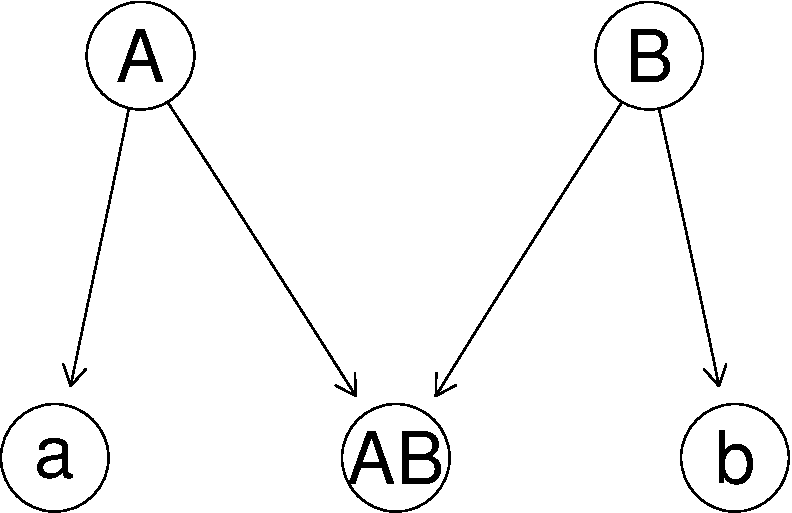
\includegraphics[width=0.6\linewidth]{conjunction-paradox_files/figure-latex/fig:conjunctionDAG-1} \end{center}
\caption{DAG of the conjunction set-up, with the usual independence assumptions built in.}
\label{fig:conjunctionDAG}
\end{figure}

The structure of the network is rather natural because each piece of
evidence bears on its hypothesis and is probabilistically independent
conditional on one of the hypotheses. One might wonder, however, why the
arrows go from \(A\) and \(B\) into the node representing the
conjunction \(A\wedge B\). This setting captures the meaning of the
conjunction. The constraint that, for the conjunction to be true, both
\(A\) and \(B\) have to be true, can be defined using the appropriate
conditional probability table (Table \ref{tab:CPTconjunction}).

\begin{table}

\begin{tabular}{lllr}
\toprule
\multicolumn{1}{c}{} & \multicolumn{1}{c}{A} & \multicolumn{1}{c}{B} & \multicolumn{1}{c}{} \\
AB &  &  & Pr\\
\midrule
1 & 1 & 1 & 1\\
0 & 1 & 1 & 0\\
1 & 0 & 1 & 0\\
0 & 0 & 1 & 1\\
1 & 1 & 0 & 0\\
0 & 1 & 0 & 1\\
1 & 0 & 0 & 0\\
0 & 0 & 0 & 1\\
\bottomrule
\end{tabular}
\caption{Conditional probability table for the conjunction node.}
\label{tab:CPTconjunction}
\end{table}

\todo{Please use the same format for tables so that it's uniform throughout the paper; I also removed the corners, it's too much fuss}

\noindent This conditional probability table looks, essentially, like
the truth table for conjunction. The difference is that the values \(1\)
and \(0\) stand for two different things depending on where they are in
the table. In the columns corresponding to the nodes they represent node
states: true and false; in the \(\textsf{Pr}\) column they represent the
conditional probability of a given state of \(AB\) given the states of
\(A\) and \(B\) listed in the same row. For instance, take a look at row
two. It says: if \(A\) and \(B\) are both in states 1, then the
probability of \(AB\) being in state 0 is 0. In principle we could use
`true' and `false' instead of 1 and 0 to represent states, but the
numeric representation is easier to use in programming, which we do
quite a bit in the background, so the reader might as well get used to
this harmless ambiguity. For binary nodes, we will consistently use `1'
and `0' for the states, it's just probabilities that in this case end up
being extreme.

To eliminate the assumption of independence between the two claims,
while holding everything else fixed, it is enough to draw an arrow
between \(A\) and \(B\) (Figure \ref{fig:conjunctionDAG2}). The two
Bayesian networks provide a compact representation of the class of
models we will be concerned with in this chapter.

\begin{figure}[h]

\begin{center}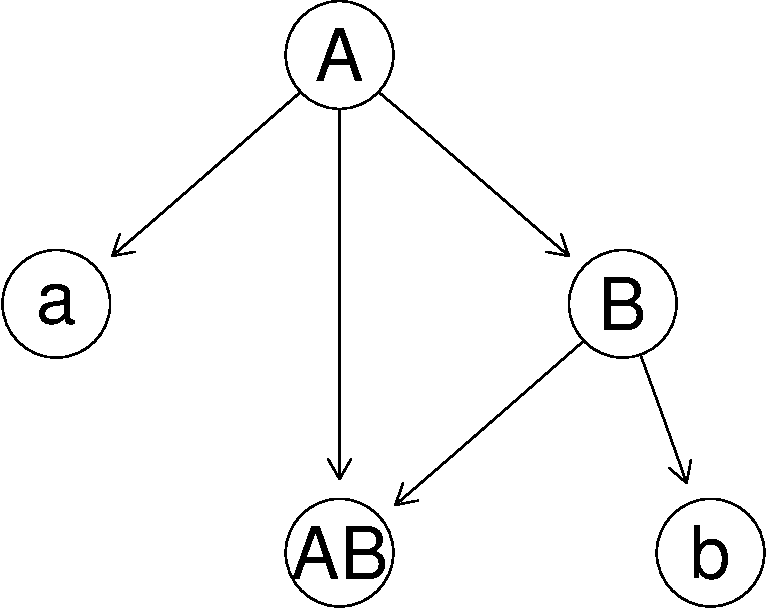
\includegraphics[width=0.6\linewidth]{conjunction-paradox_files/figure-latex/fig:conjunctionDAG2-1} \end{center}
\caption{DAG of the conjunction set-up, without independence between $A$ and $B$.}
\label{fig:conjunctionDAG2}
\end{figure}

\hypertarget{conjunction-principle-with-hypotheses-and-evidence}{%
\subsection{Conjunction principle with hypotheses and
evidence}\label{conjunction-principle-with-hypotheses-and-evidence}}

So far the discussion proceeded without mentioning explicitly the
evidence presented in support of the different claims that constitute
the allegation of wrongdoing. This is, however, a simplification, as no
evidential relations were involved. Once we pay attention to them, a
plausible candidate for the conjunction principle seems to be as
follows:

\[\text{S[$a, A$] and S[$b, B$] $\Leftrightarrow$ S[$a \wedge b, A\wedge B$]},\]

\noindent where \(\text{S}[e, H]\) means that evidence \(e\) establishes
hypothesis \(H\) by standard \(S\).

Understood in terms of a threshold put on posterior probability, the
conjunction principle above fails in some
cases.\todo{Please use vert for conditional probability. I changed this here.}
For suppose that given their respective pieces of evidence \(a\) and
\(b\), both claims \(A\) and \(B\) are sufficiently probable (for a
fixed threshold \(t\)), \(\pr{A \vert a}>t\) and \(\pr{B \vert b}>t\).
It does not generally follow that \(A \et B\) is sufficiently probable
given combined evidence \(a\et b\). With suitable indepedence
assumptions (\eqref{eq:I1} and \eqref{eq:I2}) we have: \begin{align*}
\pr{A \wedge  B \vert a \wedge b}& =\pr{A \vert a \wedge b} \times \pr{B \vert  a \wedge b \wedge A}\\
 & = \pr{A \vert a} \times \pr{B \vert  b}
 \end{align*} \noindent Of course, these relationships of independence
do not always hold, but they do sometimes. For example, in an aggravated
assault case, evidence \(a\) could be a witness testimony that the
defendant physically injured the victim (claim \(A\)), and \(b\)
evidence that the defendant knew that the victim was a firefighter
(claim \(B\)), for example, another testimony that the defendant earlier
called the firefighther for help. Presumably,
\(\pr{A \vert a}=\pr{A \vert a \wedge b}\) because the fact that the
defendant called a firefighter for help (\(b\)) does not make it more
(or less) likely that he would physically injure him (\(A\)). Further,
\(\pr{B \vert b}=\pr{B \vert a \wedge b \wedge A}\) because the fact
that the defendant injured the victim (\(A\)) and there is a testimony
to that effect (\(a\)) does not make it more (or less) likely that the
victim was a firefighter (\(B\)).

Given these assumptions, if---as is normally the case---neither
\(\pr{A \vert a}\) nor \(\pr{B \vert b}\) equal 1, then
\[\pr{A \wedge B \vert a \wedge b}< \pr{A \vert a} \;\ \& \;\ \pr{A \wedge B \vert a \wedge b} < \pr{B \vert b}. \]
This is another manifestation of the difficulty about conjuction. If
each piece of evidence \(a\) and \(b\) establishes claims \(A\) and
\(B\) with probability .95, the combined evidence \(a\et b\) may fail
establish the conjuction \(A\et B\) with probability .95. The
conjunction principle fails here, if the standard of proof is to be
formulated in terms of a threshold on posterior probability.

Even if the independence assumptions are dropped, the difficulty about
conjunction still arises in a number of circumstances. Suppose evidence
\(a\et b\) establishes claim \(A\) and also claim \(B\), separately,
right above the probability threshold \(t\). Since
\(\pr{A \wedge B \vert a \wedge b} =\pr{A \vert a \wedge b} \times \pr{B \vert a \wedge b \wedge A}\),
it follows that \(\pr{A \wedge B \vert a \wedge b}\) might be below
\(t\) if the factors on the right-hand side are below 1 and separate
posteriors are very close to \(t\).

\hypertarget{evidential-strength-approach-to-the-conjunction-problem}{%
\section{Evidential Strength approach to the conjunction
problem}\label{evidential-strength-approach-to-the-conjunction-problem}}

We have seen that aggregation fails if the standard of proof is
understood as a posterior probability threshold. Legal probabilists
cannot justify aggregation if they equate the standard of proof to such
threshold. The alternative is to think of proof standards as sufficiency
criteria for how strong the evidence should be in order to justify a
finding of criminal or civil liability. Instead of a posterior
probability threshold, legal probabilists can formalize the standard of
proof using a probabilistic measure of evidential strength. Will this
move vindicate the conjunction principle on probabilistic grounds
contrary to what Cohen thought? As we shall see, the answer to this
question is complicated.

Suppose the standard of proof is no longer understood as a threshold on
the posterior probability given the evidence, but rather, as a threshold
on evidential strength. Two common probabilistic measures of evidential
strength are the Bayes factor and the likelihood ratio. We discussed
this topic in earlier chapters (REFER TO EARLIER CHAPTERS). As will
become clear later, under plausible assumptions, these measures of
evidential strength validate one direction of the conjunction principle:
aggregation. If \(a\) is sufficiently strong evidence in favor of \(A\)
and \(b\) is sufficiently strong evidence in favor of \(B\), then
\(a\wedge b\) is sufficiently strong evidence in favor of the
conjunction \(A \wedge B\). In fact, the evidential support for the
conjunction will often exceed that for the individual claims, a point
already made by Dawid (1987):

\begin{quote} suitably measured, the support supplied by the conjunction of several independent testimonies exceeds that supplied by any of its constituents.
 \end{quote}

\noindent Dawid thought this fact was enough for the conjuction paradox
to `evaporate.' This is true since so long as we are only concerned with
vindicating one direction of the conjunction principle, aggregation.
That is, probability theory justifies this claim: if distinct items of
evidence \(a\) and \(b\) constitute sufficiently strong evidence for
claims \(A\) and \(B\), so does the conjunction \(a\wedge b\) for the
composite claim \(A\wedge B\) (although, there are some caveats and
extra assumptions for this to hold).

Unfortunately, we will show that on the evidential strength reading, the
other direction of the conjunction principle, distribution, does not
hold. If \(a \wedge b\) is sufficiently strong evidence in favor of
\(A \wedge B\), it does not follow that \(a\) is sufficiently strong
evidence in favor of \(A\) or \(b\) sufficiently strong evidence in
favor of \(B\). It is not even true that, if \(a \wedge b\) is
sufficiently strong evidence in favor of \(A \wedge B\), then
\(a\wedge b\) is sufficiently strong evidence in favor of \(A\) or
\(B\). This is odd. It would mean that, given a body of evidence, one
can establish beyond a reasonable doubt that \(A \wedge B\) (say the
defendant killed the victim \textit{and} did so intentionally) while
failing to establish by the same standard one of the conjuncts.

So we seem to be in a dilemma. If the standard of proof is understood as
a threshold relative to the posterior probability, the conjunction
principle fails because aggregation fails while distribution succeeds.
If, on the other hand, the standard of proof is understood as a
threshold relative to standard measures of evidential strength, the
conjuction principle fails because distribution fails while aggregation
succeeds. From a probabilistic perspective, it seems impossible to
capture both directions of the conjunction principle.

Before we discuss this more general challenge, let us explore how
aggregation succeeds and distribution fails on the evidential strength
approach. We will first investigate to what extent Dawid's was right in
claiming that `suitably measured, the support supplied by the
conjunction of several independent testimonies exceeds that supplied by
any of its constituents'. Next, we will show---perhaps
surprisingly---that after switching from posterior probabilities to
measures of evidential support, another paradox, what we call the
\textit{distribution paradox}, arises. The argument for these two claims
is tedious. The reader should arm themselves with patience or take our
word for it and jump ahead to the next section.

\todo{Some bits hidden, they need to be discussed elsewhere I think.}

\hypertarget{bayes-factor-and-aggregation}{%
\subsection{Bayes factor and
aggregation}\label{bayes-factor-and-aggregation}}

We will start with the Bayes factor \(\pr{E \vert H}/\pr{E}\) as our
measure of the support of \(E\) in favor of \(H\). Since by Bayes'
theorem

\[\pr{H \vert E} = \frac{\pr{E \vert H}}{\pr{E}}\times \pr{H},\]

\noindent the Bayes factor measures the extent to which a piece of
evidence increases the probability of a hypothesis. The greater the
Bayes factor (for values above one), the stronger the support of \(E\)
in favor of \(H\). Putting aside reservations about this measure of
evidential support (discussed earlier in Chapter CROSSREF), the Bayes
factor \(\pr{E \vert H}/\pr{E}\), unlike the conditional probability
\(\pr{H \vert E}\), offers a potential way to overcome the difficulty
about conjunction.

Say \(a\) and \(b\), separately, support \(A\) and \(B\)
\todo{use nicefrac for inline fractions} to degree \(s_A\) and \(s_B\)
respectively, that is, \(\nicefrac{\pr{a \vert A}}{\pr{a}}=s_A\) and
\(\nicefrac{\pr{b \vert B}}{\pr{b}=s_B}\), where both \(s_A\) and
\(s_B\) are greater than one. Does the combined evidence \(a \wedge b\)
provide at least as much support in favor of the joint claim
\(A \wedge B\) as the individual support by \(a\) and \(b\) in favor of
\(A\) and \(B\) considered separately? The combined support here is
measured by the combined Bayes factor
\(\nicefrac{\pr{a \wedge b\vert A\wedge B}}{\pr{a \wedge b}}\). The
latter, under suitable independence assumptions, equals the product of
the individual supports \(s_{A}\) and \(s_{B}\). Here is the argument:

\begin{align*}
\frac{\pr{a \wedge b\vert A\wedge B}}{\pr{a \wedge b}} & =  \frac{\pr{A \et B\vert a\wedge b}}{\pr{A \et B}}
&\mbox{\,\,\,\,\,\,\,\,\,\,\,\,\, (Bayes's theorem)}
\\
& =  \frac{\frac{ \pr{A \et B \et a \wedge b }}{\pr{a \et b}}}{\pr{A \et B}} 
&\mbox{\,\,\,\,\,\,\,\,\,\,\,\,\, (definition of conditional probability)}\\ 
& =  \frac{\frac{ \pr{A} \times \pr{B|A} \times \pr{a \vert A \wedge B} \times \pr{b \vert A \wedge B \wedge a}}{\pr{a} \times \pr{b \vert a}}}{\pr{A \et B}} 
&\mbox{\,\,\,\,\,\,\,\,\,\,\,\,\, (chain rule)}
\\ 
& =^*  \frac{\frac{\pr{A} \times \pr{B} \times \pr{a \vert A} \times \pr{b \vert B}}{\pr{a} \times \pr{b}}}{\pr{A} \times \pr{B}} 
&\mbox{\,\,\,\,\,\,\,\,\,\,\,\,\, (independencies)}\\ 
& =  \frac{\pr{a |A}}{\pr{a}} \times \frac{\pr{b |B}}{\pr{b}} 
&\mbox{\,\,\,\,\,\,\,\,\,\,\,\,\, (algebraic manipulation)} \\
s_{AB}& =  s_{A}\times s_{B} 
 \end{align*}

\noindent The step marked by the asterisk rests on some of the
independence assumptions codified in the Bayesian network in Figure
\ref{fig:conjunctionDAG}, namely: \eqref{eq:indAB}, \eqref{eq:I4}, and
\eqref{eq:I5}.

\noindent  Thus, under suitable independence assumptions, the combined
support \(s_{AB}\) will always be higher than the individual support so
long as \(s_{A}\) and \(s_{B}\) are greater than one, that is, if the
individual piece of evidence positively support their respective
hypotheses. This result can be generalized beyond two pieces of
evidence. Figure \ref{fig:bfconjunction5}compares the Bayes factor of
one item of evidence, say \(\nicefrac{\pr{a \vert A}}{\pr{a}}\) with the
combined Bayes factor for five items of evidence, say
\(\nicefrac{\pr{a_1 \wedge \dots \wedge a_5 \vert A_1 \wedge \dots \wedge A_5}}{\pr{a_1\wedge \dots \wedge a_5}}\),
for different values of sensitivity and specificity of the evidence. The
latter always exceeds the former, as soon as the individual pieces of
evidence support the individual hypotheses (the order is reversed if it
does not, and evidence with sensitivity\(=\)specificity\(=.5\) results
in Bayes factor 1, no matter what the prior is or how many items of
evidence there are). Dawid's claim that `the support supplied by the
conjunction of several independent testimonies exceeds that supplied by
any of its constituents' holds, again granted suitable independence
assumptions.

\todo{please use meaningful variable names, I revised s1 and s2 to sensitivity and specificity}
\begin{figure}[h]

\begin{center}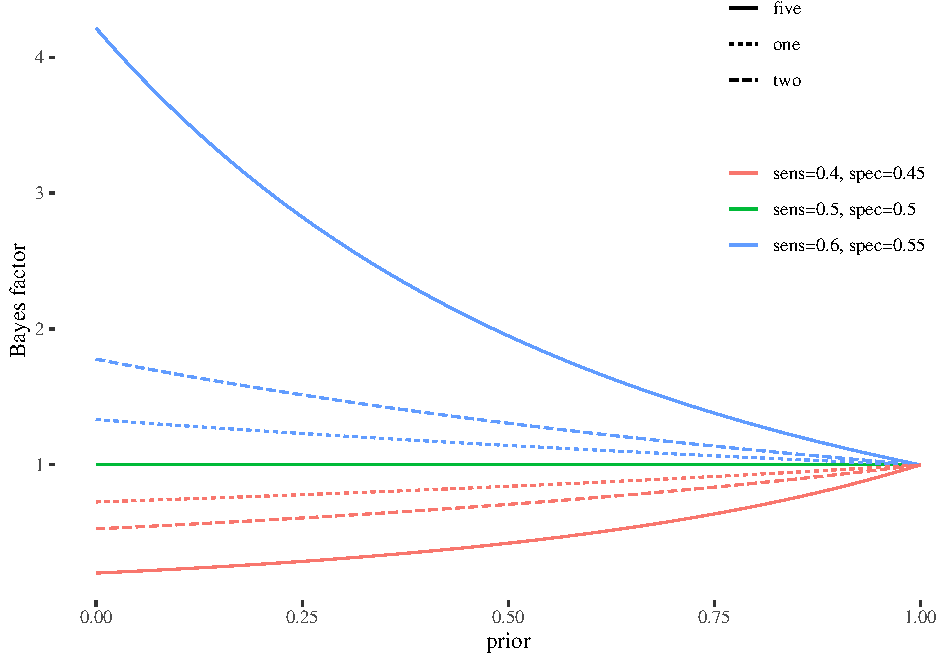
\includegraphics[width=0.9\linewidth]{conjunction-paradox_files/figure-latex/bfconjunction5-1} \end{center}
\caption{BF for varying number of items of evidence and test qualities, with the usual independence assumptions.}
\label{fig:bfconjunction5}
\end{figure}

What happens if \(A\) and \(B\) are not necessarily probabilistically
independent as in the Bayesian network in Figure
\ref{fig:conjunctionDAG2}? The claim still holds under weaker
independence assumptions in the background.
\ali{double check, are these d-sep in the second network?}

\begin{fact}
Assuming \eqref{eq:I3}, \eqref{eq:I4} and \eqref{eq:I6}, if $\pr{B\vert b\et a } > \pr{B\vert a}$ and $\pr{A\vert a \et b} > \pr{A \vert b}$, we have:
\[S_{AB}> \frac{\pr{a \vert A}}{\pr{a}}, \frac{\pr{b\vert B}}{\pr{b}}\]
\end{fact}
\todo{M: What does comma mean?}

\noindent \textbf{Argument.} First, notice the following holds given
\eqref{eq:I3} and \eqref{eq:I4}: \begin{align}
\frac{\pr{a \wedge b\vert A\wedge B}}{\pr{a \wedge b}} & =  \frac{\pr{a \vert A}}{\pr{a}} \times \frac{\pr{b \vert B}}{\pr{b\vert a}} \\
s^{'}_{AB}& =  s_{A}\times s^{'}_{B},  \label{eq:BFdep}
 \end{align}

\noindent  where factor \(s_{B}= \nicefrac{\pr{b \vert B}}{\pr{b}}\) was
replaced by
\(s^{'}_{B}=\nicefrac{\pr{b \vert B}}{\pr{b\vert a}}\).\footnote{The
  difference between \$s\_\{B\} and \(S^{'}_{B}\) is that \(b\) need not
  be probabilistically independent of \(a\), and thus there is no
  guarantee that \(\pr{b \vert a}=\pr{a}\). In fact, \(s^{'}_{B}\) is
  usually lower than \(s_{B}\) because \(\pr{b \vert a} > \pr{b}\)
  (assuming, at least, \(a\) and \(b\) are convergent pieces of
  evidence; SEE DISCUSSION IN EARLIER CHAPTERS ON CROSS-EXAMINATION AND
  CORROBORATION). At the same time, \(s^{'}_{B}\) should still be
  greater than one if \(b\) positively supports \(B\) even conditional
  on \(a\). Note that
  \(\frac{\pr{b \vert B}}{\pr{b\vert a}}=\frac{\pr{b \vert B \wedge a}}{\pr{b\vert a}}\),
  by independence \eqref{eq:I6}. Further, by Bayes' theorem,
  \(\pr{B \vert b \wedge a} = \frac{\pr{b \vert B \wedge a}}{\pr{b\vert a}} \times \pr{B\vert a}\),
  so \(\pr{B\vert b\et a}\) is obtained by multiplying \(\pr{B\vert a}\)
  by \(s^{'}_{B}\). In other words, the claim that
  \(\frac{\pr{b \vert B}}{\pr{b\vert a}}>1\) is equivalent to the claim
  that \(\pr{B \vert b \wedge a}> \pr{B\vert a}\). The latter is
  plausible in this context, since \(b\) should still raise the
  probability of \(B\) even in conjunction with \(a\), or else \(b\)
  would be useless evidence.}
\ali{check if d-sep in this fn holds in the second bn} Hence,
\(s^{'}_{AB}\) should be greater than one provided \(s_A\) and \(s_B\)
are both greater than one.
\todo{M: Do we show that the joint support exceeds 
the LOWEST of the individual support? Unclear} Note that the reasoning
behind \eqref{eq:BFdep} is symmetric and so the assumed inequalities
give the result marked by the braces: \begin{align*}
\frac{\pr{a \wedge b\vert A\wedge B}}{\pr{a \wedge b}} & =  \frac{\pr{a \vert A}}{\pr{a}} \times \underbrace{\frac{\pr{b \vert B}}{\pr{b\vert a}}}_{>1}  = \frac{\pr{b \vert B}}{\pr{b}} \times \underbrace{\frac{\pr{a \vert A}}{\pr{a\vert b}}}_{>1}
\end{align*} \textbf{Argument ends.}

\todo{Introduce simulations, illustrate results for aggregation and BF without independence here}

\hypertarget{likelihood-ratio-and-aggregation}{%
\subsection{Likelihood ratio and
aggregation}\label{likelihood-ratio-and-aggregation}}

Let's now see what happens if we replace the Bayes factor with the
likelihood ratio, another probabilistic measure of evidential support,
extensively discussed in Chapter XXX \todo{REF} As we shall understand
it here, the likelihood ratio compares the probability of the evidence
on the assumption that a hypothesis of interest is true and the
probability of the evidence on the assumption that the negation of the
hypothesis is true, that is,
\(\nicefrac{\pr{E \vert H}}{\pr{E \vert \neg H}}\). The greater the
likelihood ratio (for values above one), the stronger the evidential
support in favor of the hypothesis (as contrasted to the its negation).
We can think of the the likelihood rato as the following:

\[\frac{\textit{sensitivity}}{\textit{1- specificity}}\]

\noindent Unlike the Bayes factor, the likelihood ratio is not sensitive
to the
priors\todo{Rafal: read the sensitivity paper and check fn.}\footnote{At least so long as sensitivity and specificity are not}.
In this sense, it is a more suitable measure if we want to factor out
the effects that priors may have on the assessment of evidential
strength. What is the combined likelihood ratio and how does it behave?

\todo{This "short lived" bit was too strong, and too distracting at this point, commented out.}

\begin{fact} If independence assumptions \ali{check whic of these d-sep hold in the first and in the second BN}  \eqref{eq:I3a}, \eqref{eq:I4a},  \eqref{eq:I4b}, \eqref{eq:I4c}, \eqref{eq:I5}, \eqref{eq:I5a}, \eqref{eq:I5b}   and \eqref{eq:I5c} hold, the combined likelihood ratio is:
 \begin{align}\label{eq:jointLR}
\frac{\pr{a \wedge b \vert A\wedge B}}{\pr{a \et b\vert \neg (A\et B)}} & = \frac{\pr{a \vert A} \times \pr{b \vert B}}{\frac{\pr{\neg A}\pr{B \vert \neg A} \pr{a \vert \neg A}\pr{b \vert B} + \pr{A}\pr{\neg B \vert A} \pr{a \vert A }\pr{b \vert \neg B} + \pr{\neg A}\pr{\neg B \vert \neg A } \pr{a \vert \neg A}\pr{b \vert \neg B}}{\pr{\neg A}\pr{B \vert \neg A} + \pr{A}\pr{\neg B \vert A } + \pr{\neg A}\pr{\neg B \vert \neg A} } }
 \end{align}
\noindent If, further the hypotheses are independent in the sense of  \label{eq:indAB} this reduces to:
 \begin{align}\label{eq:jointLR2}
\frac{\pr{a \wedge b \vert A\wedge B}}{\pr{a \et b\vert \neg (A\et B)}} & = \frac{\pr{a \vert A} \times \pr{b \vert B}}{\frac{\pr{\neg A}\pr{B} \pr{a \vert \neg A}\pr{b \vert B} + \pr{A}\pr{\neg B} \pr{a \vert A }\pr{b \vert \neg B} + \pr{\neg A}\pr{\neg B} \pr{a \vert \neg A}\pr{b \vert \neg B}}{\pr{\neg A}\pr{B} + \pr{A}\pr{\neg B} + \pr{\neg A}\pr{\neg B} } }
 \end{align}
 \end{fact}

\noindent \textbf{Argument.} The numerator can be computed as follows:
\begin{align*}
\pr{a \wedge b\vert A\wedge B} & =  \frac{\pr{A \et B \et a\et b}}{\pr{A \et B}}
&\mbox{\,\,\,\,\,\,\,\,\,\,\,\,\, (conditional probability)}
\\
&= \frac{   \pr{A} \times \pr{B\vert A} \times \pr{a \vert A \wedge B} \times \pr{b \vert A \wedge B \wedge a} }{\pr{A} \times \pr{B \vert A}}
&\mbox{\,\,\,\,\,\,\,\,\,\,\,\,\, (chain rule)}
\\
& = \frac{\pr{A} \times \pr{B \vert A} \times \pr{a \vert A} \times \pr{b \vert B}}{\pr{A}  \times \pr{B \vert A}} 
&\mbox{\,\,\,\,\,\,\,\,\,\,\,\,\, (independencies \eqref{eq:I3a} and \eqref{eq:I5})}
\\
& = \pr{a \vert A} \times \pr{b \vert B} 
&\mbox{\,\,\,\,\,\,\,\,\,\,\,\,\, (algebraic manipulation)}
 \end{align*}

The numerator clearly does not depend on the prior probability of
\(A\wedge B\). We call it \textit{combined sensitivity}, and given the
independence assumptions it simply results from multiplying the
sensitivity of the individual items of evidence, \(a\) and \(b\),
relative to their respective hypotheses, \(A\) and \(B\).

The denominator is more involved:

\scalebox{.85}{\parbox{1\linewidth}{
\begin{align*}
\pr{a \et b\vert \neg (A\et B)} & = \frac{\pr{a \et b \et \neg (A\et B)}}{\pr{\neg (A \et B)}} 
&\mbox{\,\,\,\,\,\,\,\,\,\,\,\,\, (conditional probability)}\\
& = \frac{\pr{a \et b \et \neg A\et B} +  \pr{a \et b \et A\et \neg B} + \pr{a \et b \et \neg A\et \neg B}  }{\pr{\neg A \et B} + \pr{A \et \neg B} + \pr{\neg A \et \neg B} } 
&\mbox{\,\,\,\,\,\,\,\,\,\,\,\,\, (logic \& additivity)}
\end{align*}
}}

\noindent Now consider the first summand from the numerator:
\begin{align*}
\pr{a \et b \et \neg A\et B} & = \pr{\n A} \pr{B \vert \n A} \pr{a \vert \n A \et B} \pr{b\vert a \et \n A \et B} &\mbox{\,\,\,\,\,\,\,\,\,\,\,\,\, (chain rule)} \\ & = 
\pr{\neg A}\pr{B \vert \neg A} \pr{a \vert \neg A}\pr{b \vert B}
&\mbox{\,\,\,\,\,\,\,\,\,\,\,\,\, (independencies \eqref{eq:I4a} and \eqref{eq:I5a})} \\
\end{align*}

The simplification of the other two summanda is analogous (albeit with
slightly different independence assumptions---\eqref{eq:I4b} and
\eqref{eq:I5b} for the second one and \eqref{eq:I4c} and \eqref{eq:I5c}
for the third. Once we plug these into the denominator formula we get:

\scalebox{.85}{\parbox{1\linewidth}{
\begin{align*}
\pr{a \et b\vert \neg (A\et B)} & = \frac{\pr{\neg A}\pr{B \vert \neg A} \pr{a \vert \neg A}\pr{b \vert B} + \pr{A}\pr{\neg B \vert A} \pr{a \vert A }\pr{b \vert \neg B} + \pr{\neg A}\pr{\neg B \vert \neg A } \pr{a \vert \neg A}\pr{b \vert \neg B}}{\pr{\neg A}\pr{B \vert \neg A} + \pr{A}\pr{\neg B \vert A } + \pr{\neg A}\pr{\neg B \vert \neg A} }  
 \end{align*}
}}

\noindent  \eqref{eq:jointLR2} is easily obtained from
\eqref{eq:jointLR} by \label{eq:indAB}.\\
\textbf{Argument ends.}

Because of the many variables at play, it is not easy to compare the
combined evidential support and the individual support supplied by \(a\)
and \(b\) towards \(A\) and \(B\), as measured by the individual and
combined likelihood ratio. Let's work with \eqref{eq:jointLR2}. For
illustrative purposes, we simplify: Let all the sensitivites and
specificities involved be the same and equal \(x\). In this simplified
set-up with independence assumptions in the background, the combined
likelihood ratio therefore reduces to the following, where \(\pr{A}=k\)
and \(\pr{B}=t\):

\begin{align*}
\frac{\pr{a \wedge b \vert A\wedge B}}{\pr{a \et b\vert \neg (A\et B)}} & = \frac{x^2}{\frac{(1-k)t(1-x)x + k(1-t)x(1-x) + (1-k)(1-t)(1-x)(1-x)}{ \left(1-k\right) t +\left(1-t\right) k+\left(1-k\right) \left(1-t\right)}}
 \end{align*}

\noindent In this simplified setup, the likelihood ratios can be easily
plotted. As Figure \ref{fig:jointLRMarcello} shows, the combined
likelihood ratio varies depeding on the prior probabilities \(\pr{A}\)
and \(\pr{B}\), as expected, but always execeeds the individual
likelihood ratios whenever they are greater than one (that is, the two
piece of evidence provides positive support for their respective
hypothesis).

\begin{figure}

\begin{center}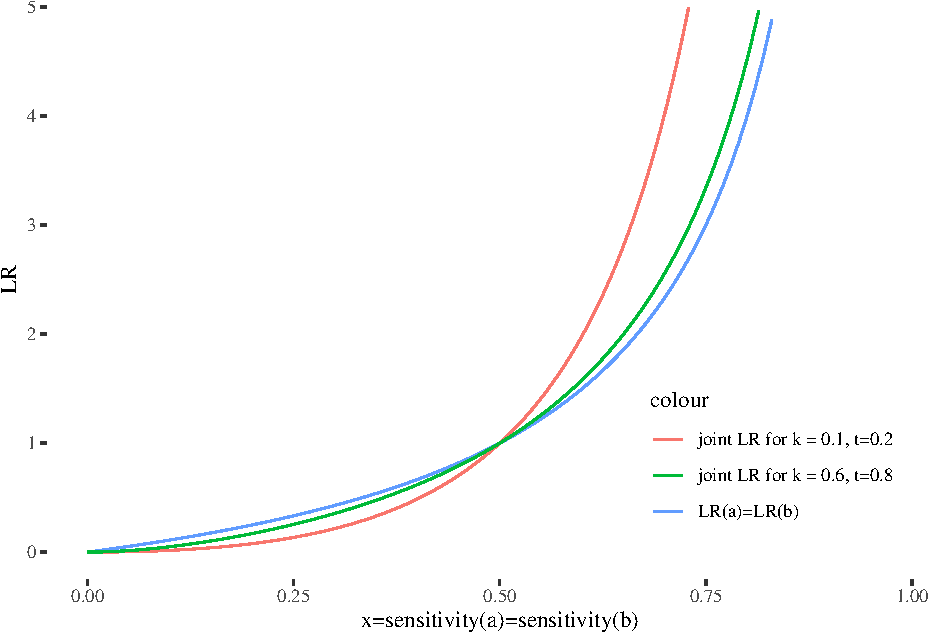
\includegraphics[width=0.9\linewidth]{conjunction-paradox_files/figure-latex/unnamed-chunk-2-1} \end{center}

\caption{Combined likelihood ratios exceeds individual Likelihood ratios as soon as sensitivity is above .5. Changes in the prior 
probabilities $t$ and $k$ do not invalidate this result.}
\label{fig:jointLRMarcello}
\end{figure}

As with the Bayes factor, the combined likelihood ratio exceeds the
individual likelihood ratios. However, this happens only as long as the
two pieces of evidence have the same sensitivity and specificity. If the
items of evidence have different levels of sensitivity and specificity,
the combined likelihood ratio never goes below the lower of the two
individual likelihood ratios, but can be lower than the higher one.

\todo{Need to add simulation results to make this argument 
fully general and drop all the simplifying assumptions (.e.g. independence or equiprobability)}

Notice that even if the composite likelihood ratio behaves somewhat
differently than the Bayes factor in being greater than the lower of the
individual likelihood ratios, rather than being greater than both of
them, Dawid's claim that `the support supplied by the conjunction of
several independent testimonies exceeds that supplied by any of its
constituents', restricted to situations in which the invidual support
levels are in fact positive, still holds.

This also entails that any likelihood ratio threshold decision standard
still satisfies aggregation: if both individual LRs are above a
threshold, then so will be the composite LR, as long as one and the same
threshold is to be used for the conjunction and for the conjuncts.
However, whether a single threshold should be used here is soemwhat
unclear, and this is an issue to which we will now turn.

\hypertarget{variable-evidential-strength-thresholds}{%
\section{Variable evidential strength
thresholds}\label{variable-evidential-strength-thresholds}}

Once we formulate the decision standard in terms of evidential strength
instead of posterior probabilities, the standard of proof would no
longer be formalized as a posterior probability threshold, but instead
as a threshold for the Bayes factor or for the likelihood ratio. The
threshold would no longer be a probability between 0 and 1, but rather a
number somewhere above 1. The greater this number, the more stringent
the standard of proof, for any value above one. In criminal trials, for
example, the rule of decision would be: guilt is proven beyond a
reasonable doubt if and only if the evidential support in favor of
\(H\)---as measured by the Bayes factor
\(\nicefrac{\pr{E \vert H}}{\pr{E}}\) (or by the likelihood ratio
\(\nicefrac{\pr{E\vert H}}{\pr{E \vert \n H}}\))---meets a suitably high
threshold \(t_{BF}\) (\(t_{LR}\)). The obvious question at this point
is, how do we identify the appropriate
threshold?\todo{will at some point take a look at "Bayesian Choice"}

One advantage of the posterior probability threshold was that in its
choice one could avoid, at least to some extent, the charge of
arbitrariness by plugging in decision-theoretic considerations and
deriving a threshold from a cost-benefit analysis.

Can we do something analogous for BF or LR? Well, in a sense, yes. If we
are able to derive \(t_BF\) or \(t_LR\) thresholds from a posterior
probability threshold, they---it seems--will be as justified by decision
theoretic-considerations that the threshold we started with. How to go
about it?
\todo{I'm now thinking: wouldn't this make $t$ movable as well though? Need to discuss.}

First, Bayes factor.
\todo{Use textsf, or even better mathsf for text inside math} Since
\(\textsf{posterior }=\textsf{ Bayes factor }\times \textsf{ prior}\),
the Bayes factor threshold can be determined as follows:
\begin{align*}t_{BF} & = \frac{t}{\textsf{prior}}
\end{align*}

\noindent The higher the prior probability, the lower \(t_{BF}\).
Whether this is a desirable property for a decision threshold can be
questioned, but a similar point holds about the posterior threshold
\(t\): the higher the prior probability, the easier to meet the
posterior threshold.

Now, likelihood ratio. By the odds version of Bayes' theorem,
\begin{align*}
\textsf{posterior odds} & = \textsf{likelihood odds} \times \textsf{prior odds},
\end{align*} and thus
\begin{align*}\frac{\textsf{posterior odds}}{\textsf{prior odds}} = \textsf{likelihood ratio}.
\end{align*} If the posterior ratio is fixed at, say \(t/1-t\),
\(t_{LR}\) can be obtained as follows:
\begin{align*}t_{LR} & = \frac{\nicefrac{t}{1-t}}{\textsf{prior odds}}.
\end{align*}

\noindent Just as the Bayes factor, the likelihood ratio threshold will
therefore varywith the prior. The higher the prior, the lower the
likelihood ratio threshold.

Now, we would like a standard of proof to be in principle applicable to
all factual claims under consideration. In particular, if we consider a
conjunction \(A\et B\), we should have a standard that makes sense not
only when applied to \(A\et B\), but also when applied to \(A \et B\).
But now notice that in the current set-up evidential strength thresholds
vary with priors, and clearly the priors for \(A\) and \(B\) will differ
from the priors on \(A\et B\). This suggests that as long as we want
\(t_{BF}\) and \(t_{LR}\) to be decision-theoretically justified by
being derived from a decision-theoretically justified posterior
probability threshold, the threhsolds for individual claims
(\(t_{BF}^A\) and \(t_{LR}^A\)) will differ from the thresholds for the
composite claim, \(t_{BF}^{A\wedge B}\) and \(t_{LR}^{A\wedge B}\) .

The conjunction principles formulated in terms of BF and LR would boil
down to:
\begin{align*} \frac{\pr{a \vert A }}{\pr{a}}>t^A_{BF} &\mbox{ and } 
\frac{\pr{ b \vert B}}{\pr{b}}>t^B_{BF} \mbox{ iff } 
\frac{\pr{a \et b \vert A \et B}}{\pr{a \et b}}>t^{A\wedge B}_{BF} \\
 \frac{\pr{a \vert A }}{\pr{a \vert \n A}}>t^A_{LR} &\mbox{ and } 
\frac{\pr{ b \vert B}}{\pr{b\vert B}}>t^B_{LR} \mbox{ iff } 
\frac{\pr{a \et b \vert A \et B}}{\pr{a \et b\vert \n (A \et B)}}>t^{A\wedge B}_{LR} \\
\end{align*}

Now, consider the individual claims \(A\) and \(B\) and their
conjunction \(A \wedge B\), assuming the independence relations required
for Facts \ali{REF} and \ali{REF} hold. Consider a posterior threshold
of \(.95\) as might be appropriate in a criminal case.

\todo{please use nicefrac for inline fractions}

If \(A\) and \(B\) both have a prior probability of, say \(.1\), the
threshold \(t^A_{BF}=t_{BF}^B=\nicefrac{.95}{.1}=9.5\) for \(A\) or
\(B\) individually. The composite claim \(A \wedge B\) will be
associated with the threshold
\(t^{A\wedge B}_{BF}=\nicefrac{.95}{(.1\times .1)}=95\), a much higher
value. But if each individual claim meets its Bayes factor threshold of
9.5 and the two claims are independent, the joint Bayes factor would
result from the multiplication of the individual Bayes factors, that is,
\(9.5 \times 9.5=90.25\). This is not quite enough to meet
\(t^{A\wedge B}_{BF}=95\).

The difference grows as (i) the prior probability of the individual
claims decreases, (ii) as the posterior threshold \(t\) decreases, and
(iii) as the number of constituents claims increases. For two
constituents, the combined Bayes factor remains only \(5\%\) below the
value needed to meet \(t_{BF}^{A\wedge B}\). The difference at here is
between \(t_{BF}^{A\wedge B}=\nicefrac{.95}{p^2}\) and
\(t_{BF}^{A}*t_{BF}^{B}=(\nicefrac{.5}{p})^{2}\). Note that
\(\frac{\nicefrac{.95}{p^2} - (\nicefrac{.5}{p})^{2}}{\nicefrac{.95}{p^2}}=.05\),
for any value of the prior \(p\). Given five constituent claims,
\(\frac{\nicefrac{.95}{p^5} - (\nicefrac{.95}{p})^{5}}{\nicefrac{.95}{p^5}}=.18\).
Now, say \(t=.5\). Even with just two claims,
\(t^{A\wedge B}_{BF}=.5/(.1*.1)=50\), but
\(t^A_{BF}*t_{BF}^B=(.5/.1)*(.5/.1)=25\), only half of the required
value.

An analogous point will hold for the likelihood ratio. Say \(A\) and
\(B\) have prior probabilities of \(.2\) and \(.3\) respectively. On
this approach, the likelihood ratio threshold for \(A\) and \(B\) will
be \(t_{LR}^{A}\approx 76\) and \(t_{LR}^{B}a\approx 44\). The
likelihood ratio threshold for the composite claim \(A \wedge B\) will
be \(t^{A\wedge B}_{LR}\approx 297\). Now suppose the individual
likelihood ratios meet their threshold and respective sensitivities and
specificities are identical. For \(t_{LR}^{A}\) to be met, evidence
\(a\) should have sensitivity of at least 0.988. For \(t_{LR}^{B}\) to
be met, evidence \(b\) should have sensitivity 0.978. Now with these
separate sensitivies, The combined likelihood ratio equals about 145,
far short that what the threshold \(t^{A\wedge B}_{LR}\) requires,
namely a likelihood ratio of 297.

Things don't get better with a lower posterior threshold. Say \(t= .5\),
as might be appropriate in a civil case. The likelihood ratio thresholds
for \(A\) and \(B\) will be \(t_{LR}^{A}\approx 4\) and
\(t_{LR}^{B}a\approx 2.3\). The likelihood ratio threshold for the
composite claim \(A \wedge B\) will be
\(t^{A\wedge B}_{LR}\approx 15.6\). To ensure that \(t_{LR}^{A}\) is
met, evidence \(a\) should have a sensitivity of at least 0.8, and to
ensure that \(t_{LR}^{B}\) is met, evidence \(b\) should have a
sensitivity of at least 0.7. To ensure that \(t_{LR}^{B}\) is met,
evidence \(b\) should have a sensitivity of at least 0.7. With these
parameters, the combined likelihood ratio equals about 5, far short that
what the threshold \(t^{A\wedge B}_{LR}\) requires, namely a likelihood
ratio of 15.

The general lesson here is this. If we want the choice of evidential
strength threshold to be informed by decision-theoretic considerations
(as might be advisable), and we do so by deriving them from
decision-theoretically justified posterior thresholds, the evidential
strength thresholds become variable: they depend on priors. If in fact
we then do keep track of which threshold is supposed to be used for
which claim, aggregation still fails: there will be cases in which the
conjuncts taken separately satisfy the decision standard, while the
conjunction does not.
\todo{Question: how does Kaplow think about it? Does he only derive threshold for the ultimate claim? I don't remember now.}

Perhaps, this is not the path that the proponent of the evidential
strength approach would take anyway. After all, if your evidential
strength thresholds mirror posterior threshold, it should not be deeply
surprising if they run into similar problems. So what would happen if
instead, we insisted that the evidential strength thresholds should be
kept fixed?

\hypertarget{fixed-evidential-strength-threshold}{%
\section{Fixed evidential strength
threshold}\label{fixed-evidential-strength-threshold}}

The alternative here is to fix the evidential strength threshold
regardless of the prior probability of the claim of interest. This
raises the difficult question of how to fix the threshold irrespective
of the priors. Standard decision theory can no longer be used. As it
turns out, even if the question can be satisfactorily answered, the
fixed threshold approach gives rise to a complication that proves fatal.

If the standard of proof is formalized using a fixed threshold for the
Bayes factor or for the likelihood ratio, the conjunction principle
would boil down to one of these:

\begin{align*} \frac{\pr{a \vert A }}{\pr{a}}>t_{BF} &\mbox{ and } 
\frac{\pr{ b \vert B}}{\pr{b}}>t_{BF} \mbox{ iff } 
\frac{\pr{a \et b \vert A \et B}}{\pr{a \et b}}>t_{BF} \\
 \frac{\pr{a \vert A }}{\pr{a \vert \n A}}>t_{LR} &\mbox{ and } 
\frac{\pr{ b \vert B}}{\pr{b\vert B}}>t_{LR} \mbox{ iff } 
\frac{\pr{a \et b \vert A \et B}}{\pr{a \et b\vert \n (A \et B)}}>t_{LR} \\
\end{align*}

\noindent The left-to-right direction---aggregation---will hold for any
thresholds \(t_{BF}\) or \(t_{LR}\) greater than one, as Facts \ali{REF}
and \ali{REF, not sure how many we end up with, double check} entail.

This is an improvement. After all, aggregation could not be justified
using posterior probabilities \(\pr{A \vert a}\) and \(\pr{B \vert b}\)
nor could it be justified generally using a variable Bayes factor
threshold. So it is an advantage of the fixed evidential strength
threshold approach that it can justify this direction of the conjunction
principle.

However, the right-to-left direction---distribution---has now become
problematic. Recall that we can distinguish at least two versions of the
distribution principle if we take the evidential support into account:
\begin{align}
\text{If S[$a \wedge b, A\wedge B$], then S[$a, A$] and S[$b, B$].} \tag{DIS1}\\
 \text{If S[$a \wedge b, A\wedge B$], then S[$a \wedge b, A$] and S[$a \wedge b, B$].} \tag{DIS2}
\end{align}

We will think of both of them. Let us start with (DIS1) first, still
working with the independence assumptions in the background for the sake
of simplicity. Suppose the combined Bayes factor,
\(\frac{\pr{a \et b \vert A \et B}}{\pr{a \et b}}\), barely meets the
threshold. The individual support, say
\(\frac{\pr{a \vert A}}{\pr{a}}\), could be still below the threshold
unless \(\frac{\pr{b \vert B}}{\pr{b}}=1\) (which should not happen if
\(b\) positively supports \(B\)).

The problem for likelihood ratio is analogous. For suppose evidence
\(a \et b\) supports \(A \et B\) to the required threshold \(t\). The
threshold in this case should be some order of magnitude greater than
one. If the combined likelihood ratio meets the threshold \(t_{LR}\),
one of the individual likelihood ratios may well be below \(t_{LR}\).
So---if the standard of proof is interpreted using evidential support
measured by the likelihood ratio---even though the conjuction
\(A \et B\) was proven according to the desired standard, one of
individual claims might not. (DIS1) in some cases fails.

Perhaps, the problem was with (DS1). Could this principle be rejected?
Maybe it is not as essential as we thought at first. Since the evidence
is not held constant, the support supplied by \(a\wedge b\) could be
stronger than that supplied by \(a\) and \(b\) individually. So even
when the conjunction \(A \wedge B\) is established to the requisite
standard given evidence \(a\wedge b\), it might still be that \(A\) does
not meet the requisite standard (given \(a\)) nor does \(B\) (given
\(b\)). Or at least one might try to argue so.

(DS2) is less controversial, as it holds the evidence constant. This
principle is harder to deny: one would not want to claim that, holding
fixed evidence \(a\wedge b\), establishing the conjunction might not be
enough for establishing one of the conjuncts. It seems that any
formalization of the standard of proof should obey (DIS2). Yet, (DIS2)
also fails both for Bayes factor and likelihood ratio. After all, if
\(A\) and \(B\) are probabilistically independent, (DIS1) and (DIS2) are
in fact equivalent, so the counterexamples to (DIS1) work also against
(DS2).

So, curiously, on the fixed evidential strength threshold approach, no
matter whether one uses Bayes factor or likelihood ratio, there would be
cases in which, even though the conjunction \(A\et B\) is established to
the desired standard of proof, one of the individual claims fails to
meet the standard. This is odd, to say the least.

\todo{I don't think this argument worked, we can discuss this. Commented out}

\todo{M: This section seems to be missing a lot of the reasoning 
that was commented out. Is this still comprehensible? 
Not sure I can follow. Seems too brief.}

\hypertarget{the-comparative-strategy}{%
\section{The comparative strategy}\label{the-comparative-strategy}}

Instead of thinking in terms of absolute thresholds---whether relative
to posterior probabilities, the Bayes factor or the likelihood
ratio---the standard of proof can be understood comparatively. This
suggestion has been advanced by Cheng (2012) following the theory of
relative plausibility by
\textbf{REFERENCE TO ALLEN AND PARDO HERE}.\todo{Which one?} Say the
prosecutor or the plaintiff puts foward a hypothesis \(H_p\) about what
happened. The defense offers an alternative hypothesis, call it \(H_d\).
On this approach, rather than directly evaluating the support of \(H_p\)
given the evidence and comparing it to a threshold, we compare the
support that the evidence provides for two competing hypotheses \(H_p\)
and \(H_d\), and decide for the one for which the evidence provides
better support.

It is controversial whether this is what happens in all trial
proceedings, especially in criminal trials, if one thinks of \(H_d\) as
a substantial account of what has happened. The defense may elect to
challenge the hypothesis put foward by the other party without proposing
one of its own. For example, in the O.J.~Simpson trial the defense did
not advance its own story about what happened, but simply argued that
the evidence provided by the prosecution, while significant on its face
to establish OJ's guilt, was riddled with problems and deficencies. This
defense strategy was enough to secure an acquittal. So, in order to
create a reasonable doubt about guilt, the defense does not always
provide a full-fledged alternative hypothesis. The supporters of the
comparative approach, however, will respond that this could happen in a
small number of cases, even though in general---especially for tactical
reasons---the defense will provide an alternative hypothesis. And even
such cases can be construed as involving a defense hypothesis, one that
is simply equivalent to the negation of \(H_p\).

Setting aside this controversy for the time being, let's first work out
the comparative strategy using posterior probabilities. More
specifically, given a body of evidence \(E\) and two competing
hypotheses \(H_p\) and \(H_d\), the probability \(\pr{H_p \vert E}\)
should be suitably higher than \(\pr{H_d \vert E}\), or in other words,
the ratio \(\nicefrac{\pr{H_p \vert E}}{\pr{H_d \vert E}}\) should be
above a suitable threshold. Presumably, the ratio threshold shoud be
higher for criminal than civil cases. In fact, in civil cases it seems
enough to require that the ratio
\(\nicefrac{\pr{H_p \vert E}}{\pr{H_d \vert E}}\) be above 1, or in
other words, that \(\pr{H_p \vert E}\) should be higher than
\(\pr{H_d \vert E}\).\todo{I'm not convinced this footnote is needed and what its point is.}\footnote{Note that $H_p$ and $H_d$ need not be one the negation of the other. 
Whenever two hypotheses are exclusive and exhaustive, $\nicefrac{\pr{H_p \vert E}}{\pr{H_d \vert E}}>1$ 
implies that $\pr{H_p \vert E}>.5$, the standard probabilistic interpretation of the preponderance standard.}

One advantage of this approach---as Cheng shows---is that expected
utility theory can set the appropriate comparative threshold \(t\) as a
function of the costs and benefits of trial decisions. For simplicity,
suppose that if the decision is correct, no costs result, but incorrect
decisions have their price. \todo{REFERENCE TO EARLIER CHAPTER 
FOR MORE COMPLEX COST STRUCTURE} The costs of a false positive is
\(c_{FP}\) and that of a false negative is \(C_{FN}\), both greater than
zero. Intuitively, the decision rule should minimize the expected costs.
That is, a finding against the defendant would be acceptable whenever
its expected costs---\(\pr{H_d \vert E} \times c_{FP}\)---are smaller
than the expected costs of an
acquittal---\(\pr{H_p \vert E}\times c_{FN}\)--- or in other words:

\[\frac{\pr{H_p \vert E}}{\pr{H_d \vert E}} > \frac{c_{FP}}{c_{FN}}.\]

\noindent In civil cases, it is customary to assume the costs ratio of
false positives to false negatives equals one. So the rule of decision
would be: find against the defendant whenever
\(\frac{\pr{H_p \vert E}}{\pr{H_d \vert E}} > 1\) or in other words
\(\pr{H_p \vert E}\) is greater than \(\pr{H_d \vert E}\). In criminal
trials, the costs ratio is usually considered higher, since convicting
an innocent (false positive) should be more harmful or morally
objectionable than acquitting a guilty defendant (false negative). Thus,
the rule of decision in criminal proceedings would be: convict whenever
\(\pr{H_p \vert E}\) is appropriately greater than \(\pr{H_d \vert E}\).

Does the comparative strategy just outlined solve the difficulty about
conjunction? We will work through a stylized case used by Cheng himself.
Suppose, in a civil case, the plaintiff claims that the defendant was
speeding (\(S\)) and that the crash caused her neck injury (\(C\)).
Thus, the plaintiff's hypothesis \(H_p\) is \(S\et C\). Given the total
evidence \(E\), the conjuncts, taken separately, meet the decision
threshold: \begin{align}
 \nonumber 
 \frac{\pr{S\vert E}}{\pr{\neg S \vert E}} > 1   & & \frac{\pr{C\vert E}}{\pr{\neg C \vert E}} > 1
\end{align} \noindent The question is whether
\(\nicefrac{\pr{S\et C\vert E}}{\pr{H_d \vert E}}>1\). To answer it, we
have to decide what the defense hypothesis \(H_d\) should be. Cheng
reasons that there are three alternative defense scenarios:
\(H_{d_1}= S\et \n C\), \(H_{d_2}=\n S \et C\), and
\(H_{d_3}=\n S \et \n C\). How does the hypothesis \(H_p\) compare to
each of them? Assuming independence between \(C\) and \(S\), we have

\begin{align}\label{eq:cheng-multiplication}
\frac{\pr{S\et C\vert E}}{\pr{S\et \n C\vert E}} & = \frac{\pr{S\vert E}\pr{C\vert E}}{\pr{S \vert E}\pr{\n C \vert E}}  =\frac{\pr{C\vert E}}{\pr{\n C \vert E}} > 1 \\
\nonumber
\frac{\pr{S\et C\vert E}}{\pr{\n S\et C\vert E}} & = \frac{\pr{S\vert E}\pr{C\vert E}}{\pr{\n S \vert E}\pr{C\vert E}}  = \frac{\pr{S\vert E}}{\pr{\n S \vert E}} > 1 \\
\nonumber
\frac{\pr{S\et C\vert E}}{\pr{\n S\et \n C\vert E}} & = \frac{\pr{S\vert E}\pr{C\vert E}}{\pr{\n S \vert E}\pr{\n C \vert E}}   > 1 
\end{align}

\noindent So, whatever the defense hypothesis, the plaintiff's
hypothesis is more probable. At least in this case, whenever the
elements of a plaintiff's claim satisfy the decision threshold, so does
their conjunction. The left-to-right direction of the conjunction
principle---what we called aggregation---has been vindicated, at least
for simple cases involving independence.

What about the opposite direction, distribution? If the threshold to be
met just 1---as might be appropriate in civil cases---distribution would
be satisfied. Suppose
\(\nicefrac{\pr{S\et C\vert E}}{\pr{H_d \vert E}}>1\), or in other
words, the combined hypothesis \(S \et C\) has been established by
preponderance of the evidence. The question is whether the individual
hypotheses have been established by the same standard, specifically,
whether \(\frac{\pr{C\vert E}}{\pr{\n C \vert E}} > 1\) and
\(\frac{\pr{S\vert E}}{\pr{\n S \vert E}} > 1\). If
\(\nicefrac{\pr{S\et C\vert E}}{\pr{H_d \vert E}}>1\), the combined
hypothesis is assumed to be more probable than any of the competing
hypotheses, in particular,
\(\nicefrac{\pr{S\et C\vert E}}{\pr{\neg S \et C \vert E}}>1\),
\(\nicefrac{\pr{S\et C\vert E}}{\pr{S \et \neg C \vert E}}>1\) and
\(\nicefrac{\pr{S\et C\vert E}}{\pr{\neg S \et \neg C \vert E}}>1\). We
have

\begin{align}\label{eq:cheng-multiplication-two}
1 < \frac{\pr{S\et C\vert E}}{\pr{S\et \n C\vert E}} & = \frac{\pr{S\vert E}\pr{C\vert E}}{\pr{S \vert E}\pr{\n C \vert E}}  =\frac{\pr{C\vert E}}{\pr{\n C \vert E}} \\
\nonumber
1 < \frac{\pr{S\et C\vert E}}{\pr{\n S\et C\vert E}} & = \frac{\pr{S\vert E}\pr{C\vert E}}{\pr{\n S \vert E}\pr{C\vert E}}  = \frac{\pr{S\vert E}}{\pr{\n S \vert E}}  \\
\nonumber
1 < \frac{\pr{S\et C\vert E}}{\pr{\n S\et \n C\vert E}} & = \frac{\pr{S\vert E}\pr{C\vert E}}{\pr{\n S \vert E}\pr{\n C \vert E}}   
\end{align}

In the first two cases, clearly, if the composite hypothesis meets the
threshold, so do the individual claims. But now consider the third case.
\(\nicefrac{\pr{S\vert E}\pr{C\vert E}}{\pr{\n S \vert E}\pr{\n C \vert E}}\)
might be strictly greater than
\(\nicefrac{\pr{C\vert E}}{\pr{\n C \vert E}}\) or
\(\nicefrac{\pr{S\vert E}}{\pr{\n S \vert E}}\). So it possible that
\(\nicefrac{\pr{S\vert E}\pr{C\vert E}}{\pr{\n S \vert E}\pr{\n C \vert E}}\)
is greater than one, while
either\(\nicefrac{\pr{C\vert E}}{\pr{\n C \vert E}}\) or
\(\nicefrac{\pr{S\vert E}}{\pr{\n S \vert E}}\) are not, say when they
are 3 and 0.5, respectively. Once again, distribution fails. And the
same problem would arise with a more stringent threshold as might be
appropriate in criminal cases.

There is a more general problem with the comparative approach worth
flagging here. Much of the heavy lifting here is done by the strategic
splitting of the defense line into multiple scenarios. Now suppose, for
illustrative purposes, \(\pr{H_p\vert E}=0.37\) and the probability of
each of the defense lines given \(E\) is \(0.21\). This means that
\(H_p\) wins with each of the scenarios, so on this approach we should
find against the defendant. But should we? Given the evidence, the
accusation is very likely to be false, because
\(\pr{\n H_p \vert E}=0.63\). The problem generalizes. If, as here, we
individualize scenarios by Boolean combinations of elements of a case,
the more elements there are, into more scenarios \(\n H_p\) needs to be
divided. This normally would lead to the probability of each of them
being even lower (because now \(\pr{\n H_p}\) needs to be ``split'\,'
between more scenarios). So, if we take this approach seriously, the
more elements a case has, the more at a disadvantage the defense is.
This seems undesirable.

MENTION THAT SINCE CHENG THOUGHT THE COMPARATIVE STRATEGY WOULD CAPTURE
INFERENCE TO THE BEST EXPLANATION IN PROBABILISTIC TERMS, THE FAILURE OF
THE COMPARATIVE STRATEGY TO CAPTURE THE CONJUNCTION PRINCIPLE IS ALSO A
FAILURE OF INFERENCE TO THE BEST EXPLANATION IN CAPTURING THE
CONJUNCTION PRINCIPLE SO LONG AS WE ASSUME THAT PLAUSIBILITY DOES NOT
CONTRADICT PROBABILITY (WHICH ALLEN AND PARDO DO GRANT)

\hypertarget{rejecting-the-conjunction-principle}{%
\section{Rejecting the Conjunction
Principle?}\label{rejecting-the-conjunction-principle}}

We have seen that various strategies that a legal probabilist can try to
use to handle the difficulty about conjunction are all problematic.
Perhaps, a different perspective should be taken here? After all, the
problem would not arise without the conjunction principle. So could
legal probabilists simply reject this principle?
\todo{add more flow once section is complete}

\hypertarget{risk-accumulation}{%
\subsection{Risk Accumulation}\label{risk-accumulation}}

In current discussions in epistemology about knowledge or justification,
a principle similar to the conjunction principle has been contested
because it appears to deny the fact that risks of error accumulate
(Kowalewska, 2021). If one is justifiably sure about the truth of each
claim considered seperataly, one should not be equally sure of their
conjunction. You have checked each page of a book and found no error.
So, for each page, you are nearly sure there is no error. Having checked
each page and found no error, can you be sure that the book as a whole
contains no error? Not really. As the number of pages grow, it becomes
virtually certain that there is at least one error in the book you have
overlooked, although for each page you are nearly sure there is no error
(Makinson, 1965). The same applies to other contexts, say product
quality control. You may be sure, for each product you checked, that it
is free from defects. But you cannot, on this basis alone, be sure that
all products you checked are free from defects. Since the risks of error
accumulate, you must have missed at least one defective product.

Risk accumulation challenges aggregation: even if the probability of
several claims, considered individually, is above a threhsold \(t\),
their conjuction need not be above \(t\). It does not, however,
challenge distribution. It seems that if all-risks-considered, you have
good reasons to accept a conjunction, no further risk is involved in
accepting any of the conjuncts separately. This is also mirrored by what
happens with probabilities: Probability theory ensures that, if the
probability of the conjunction of several claims is above \(t\), so is
the probability of each individual claim. This means that risk
accumulation does not help one to save the approaches for which
distribution fails.
\todo{I added a sentence of how this is related to previous sections, should we say sth more here? What's our take on risk accummulation?}

\todo{M: Maybe our take should be that there is an ambiguity between support and support 2. Adding more evidence and more claims strengthens support1 (aggregation holds), but more claims weaekns support2. The paradox is running both ideas toghether.}

\noindent

\hypertarget{atomistic-and-holistic-approches}{%
\subsection{Atomistic and Holistic
Approches}\label{atomistic-and-holistic-approches}}

Suppose the legal probabilist does away with the conjunction principle.
Now what? How should they define standards of proof? Two immediate
options come to mind, but neither is without problems.

Let's stipulate that, in order to establish the defendant's guilt beyond
a reasonable doubt (or civil liability by preponderance of the
evidence), the party making the accusation should establish each claim,
separately, to the requisite probability, say at least .95, without
needing to establish the conjunction to the requisite probability. Call
this the \textit{atomistic account}. On this view, the prosecution could
be in a position to establish guilt beyond a reasonable doubt without
estalishing the conjunction of different claims with a sufficiently high
probability. This account would allow convictions in cases in which the
probability of the defendant's guilt is relatively low, just because
guilt is a conjunction of several independent claims that separately
satisfy the standard of proof. For example, if each constituent claim is
established with .95 probability, a composite claim consisting of five
subclaims---assuming, as usual, probabilistic independence between
individual claims---would only be established with probability equal to
.77, a far cry from proof beyond a reasonable doubt. This is
counterintuitve, as it would allow convictions when the defendant is not
very likely to be guilty. Under the atomistic account, the composite
claim representing the case as a whole would often be established with a
probability below the required threshold. The atomistic approach is a
non-starter.

Another option is to require that the prosecution in a criminal case (or
the plaintiff in a civil case) establish the accusation as a whole---say
the conjunction of \(A\) and \(B\)---to the requisite probability. Call
this the \textit{holistic account}. This account is not without problems
either. The proof of \(A\et B\) would impose a higher requirement on the
separate probabilities of the conjuncts. If the conjunction \(A\et B\)
is to be proven with at least .95 probability, the individual conjuncts
should be established with probability higher than .95. So the more
constituent claims, the higher the posterior probability for each claim
needed for the conjunction to meet the requisite probability threshold.

We can get a sense of the difficulty by running in some numbers. Assume,
for the sake of illustration, the independence and equiprobability of
the constituent claims. If a composite claim consists of \(k\)
individual claims, these individual claims will have to be established
with probability of at least \(t^{1/k}\), where \(t\) is the threshold
to be applied to the composite
claim.\footnote{Let $p$ the probability of each constituent claim. To meet threshold $t$, the probability of the composite claim, $p^k$, should satisfy the constraint $p^k>t$, or in other words, $p>t^{1/k}$.}
For example, if there are ten constituent claims, they will have to be
proven with \(.5^{1/10}=.93\) even if the probability threshold is only
\(.5\). If the threshold is more stringent, as is appropriate in
criminal cases, say \(.95\), each individual claim will have to be
proven with near certainty. This would make the task extremely demanding
on the prosecution. If there are ten constituent claims, they will have
to be proven with \(.95^{1/10}=.995\). So the plaintiff or the
prosecution would face the demanding task of establishing each element
of the accusation beyond what the standard of proof would seem to
require.

Another problem with the holistic account is that the standard that
applies to one of the conjuncts would depend on what has been achieved
for the other conjuncts. For instance, assuming independence, if
\(\pr{A}\) is \(.96\), then \(\pr{B}\) must be at least \(.99\) so that
\(\pr{A\et B}\) is above a \(.95\) threshold. But if \(\pr{A}\) is
\(.9999\), then \(\pr{B}\) must only be greater than \(.95\) to reach
the same threshold. Thus, the holistic account might require that the
elements of an accusation be proven to different probabilities---and
thus different standards---depeding on how well other claims have been
established. This result runs counter to the tacit assumption that each
element should be established to the same standard of proof.

\begin{verbatim}
## [1] 0.933033
\end{verbatim}

\begin{verbatim}
## [1] 0.9948838
\end{verbatim}

\begin{verbatim}
## [1] 0.5987369
\end{verbatim}

We have a dilemma here: either (under the holistic approach) the
standard is too demanding on the prosecution (or the plaintiff) because
it requires the individual claims to be established to extremely high
probabilities, or (under the atomistic approach) the standard is too lax
because it allows for findings of liability when the defendant quite
likely committed no wrong. Denying the conjunction principle, then, is
not without difficulties of its own. Absent the conjunction principle,
legal probabilists should still explain how individual claims relate to
larger claims in the process of legal proof, and how the balance between
these two extreme directions is to be preserved.

\hypertarget{the-holistic-approach-revised}{%
\subsection{The holistic approach
revised}\label{the-holistic-approach-revised}}

The difficulty about conjunction begins with the assumption that each
element of the allegation has been established by the required standard.
Then, one argues that it does not follow that the conjunction has been
established by the required standard. Aggregation fails. This is the
paradox. But the force of this paradox can be limited by noting that
each element will be established by higher probability than the
conjunction because each element will have a higher prior probability,
other things being equal. Along these lines, Dawid (1987), in one of the
earliest attempts to solve the conjunction paradox from a probabilistic
perspective, wrote:

\begin{quote}
\dots it is not asking too much of the plaintiff to establish the case as a whole with a posterior probability exceeding one half, even though this means  that the several component issues must be established with much larger posterior probabilities; for the \textit{prior}  probabilities of the components will also be correspondingly larger, compared with that of their conjunction (p. 97).
 \end{quote}

THIS PART IS INCOMPLETE AND NEEDS WORK

It is worth developing Dawid's observation in greater detail. For
simplicity, assume the prosecution should establish the composite claim
\(A \wedge B\) by \(.95\) probability, where each individual claim is
probabilistically independent of the other. Say the composite claim has
a prior probability of only \(.01\). Thus, the individual claims have a
prior probability of \(.1\). If the probability threshold to be met is
\(.95\), the evidence should be strong enough to move the probability of
\(A \wedge B\) from \(.01\) to \(.95\), or in ratio form,
\(\nicefrac{.95}{.01}=95\). The same evidence should be strong enough to
move the individual claims \(A\) or \(B\) from \(.1\) to \(.95\), or in
ratio form, \(9.5\).The ratios \(95\) and \(9.5\) of posterior to prior
probabilities are equivalent to the Bayes factor. For recall that

\[\textit{posterior} = \textit{Bayes factor} \times \textit{prior}\]

Recall, also, that the Bayes factor for individual hypotheses, given a
fixed body of evidence,

This point can be made more precisely by equalizing the prior
probabilities of composite and individual claims, and by comparing the
extent to which the evidence is expected to shift the prior probability
of the composite claim compared to the equalized prior prior probability
of the individual claim. So suppose both the composite claim and the
individual claim have the same prior probability, say \(.01.\). The
Bayes factor

\begin{verbatim}
## [1] 0.1
\end{verbatim}

\begin{verbatim}
## [1] 95
\end{verbatim}

\begin{verbatim}
## [1] 9.5
\end{verbatim}

\begin{verbatim}
## [1] 90.25
\end{verbatim}

\begin{verbatim}
## [1] 188.1
\end{verbatim}

\begin{verbatim}
## [1] 17.1
\end{verbatim}

\begin{verbatim}
## [1] 289
\end{verbatim}

We think this is the right strategy.\todo{I'm not convinced.} Here we
offer a rough description of what is to follow in further chapters: our
revised version of the holistic approach, partially inspired by Dawid's
insight.

So far we have been mostly focusing on the most straightforward
probabilistic interpretation of proof standards, one that posits a
threshold on the posterior probabilities or on evidential strength of a
generic hypothesis, such as guilt or civil liability. For instance, in
criminal cases, the requirement might formulated in terms of posteriors
as follows: guilt is proven beyond a reasonable doubt provided
\(\pr{G \vert E}\) is above a suitable threshold, say .95. The threshold
is lower in civil trials. Civil liability is proven by preponderance
provided \(\pr{L \vert E}\) is above a suitable threshold, say .5.
Perhaps, the general claim \(G\) or \(L\) is sometimes split into
several consituent claims, depending on the defintion of the wrongful
act in the governing law. But this framing misses a crucial ingredient.

The claim that the defendant is guilty or civilly liable can be replaced
by a more fine-grained hypothesis about the facts involved, call it
\(H_p\), the hypothesis put foward by the prosecutor (or the plaintiff
in a civil case), for example, the hypothesis that the defendant killed
the victim with a firearm while bulglarizing the victim's apartment.
\(H_p\) can be any hypothesis which, if true, would entail the
defendanat is civilly or criminally liable (according to the governing
law). Hypothesis \(H_p\) is a more precise description of what happened
that establishes, if true, the defendant's guilt or civil
liability.\todo{Repetitive?} In defining proof standards, instead of
saying---somewhat generically ---that \(\pr{G \vert E}\) or
\(\pr{L \vert E}\) should be above a suitable threshold, a probabilistic
interpretation could read: civil or criminal liability is proven beyond
a reasonable doubt provided \(\Pr(H_p \vert E)\) is above a suitable
threshold.

This variation may appear inconsequential. But in Chapter XXX
\todo{REF?} we will argue--- perhaps surprisingly--- that it can address
the naked statistical evidence problem and the difficulty about
conjunction.

We have examined the naked statistical evidence problem in another
chapter \textbf{REFERENCE TO EARLIER HAPER}. The basic argument was
this. Consider the prisoner hypothetical. It is true that the naked
statistics make him .99 likely to be guilty, that is,
\(\pr{G \vert E_s} =.99\). It is \(.99\) likely that he is one the
prisoners who attacked and killed the guard. Notice that this a generic
claim. It is odd for the prosecution to simply assert that the prisoner
was one of those who killed the guard, without saying what he did, how
he partook in the killing, what role he played in the attack, etc. If
the prosecution offerred a more specific incriminating hypothesis, call
it \(H_p\), the probability \(\pr{H_p \vert E_{s}}\) of this hypothesis
based on the naked statistical evidence \(E_s\) would be well below
\(.99\), even though \(\pr{G \vert E_s}=.99\). The fact the prisoner on
trial is most likely guilty is an artifact of the choice of a generic
hypothesis \(G\). When this hypothesis is made more specific ---as it
should be---this probability drops significantly.

The same approach can address the difficulty about conjunction. The
tacit assumption behind the difficulty is that prosecutors or plaintiffs
should establish each element in isolation. If they manage to prove each
element to the desired standard, they have meet their burden. This is
artificial. What prosecutors or plaintiffs should do instead is to
establish a specific hypothesis from which the constituent elements
follow (almost) deductively. To illustrate, consider a Washington
statute about negligent driving:

\begin{quote}
(1)(a) A person is guilty of negligent driving in the first degree if he or she operates a motor vehicle in a manner that is both negligent and endangers or is likely to endanger any person or property, and exhibits the effects of having consumed liquor or marijuana or any drug or exhibits the effects of having inhaled or ingested any chemical, whether or not a legal substance, for its intoxicating or hallucinatory effects. 

[RCW 46.61.5249]
\end{quote}

\noindent In other words, a prosecutor who wishes to establish beyond a
reasonable doubt that the defendant is guilty of negligent driving
should establish:

\begin{quote}
(a) that the defendant operated a vehicle
(b) that, in operating a vehicle, the defendant did so in  negligente manner
(c) that, in operating a vechicle, the defendant did so in a manner likely to endanger a person pr property
(d) that the defendant---presumably, immediately after the incident--- exihibited the signs of intoxication by liquor or drugs.
\end{quote}

\noindent It would be odd for the prosecutor to go about establishig
each claim in isolation, especially because these four claims are
specific to a time and place. Clearly, the prosecutor cannot simply
establish that the defendant was operating a vehicle at some point in
time and at some other point in time the defedant exhibited signs of
intoxication. That would establish nothing. The elements to be
established must be combined in a coherent spatio-temporal narrative. So
establishing them in isolation makes little sense. Prosecutors could
establish, say, that the defendant was driving on a busy Highway 1 north
San Francisco at about 8:30 PM; the car was moving erratically left and
right, cutting across other lanes; the defendant was stopped by a police
officer who conducted a field sobriety test and used a breathylizer,
both tests showing a higher-than-normal quantity of alchool. This
narrative, if true, establishes each element of the offense. The
prosecutor's task would be to establish the narrative as a whole.
Presumably, the prosecutor could establish item (a) and (b) separately,
but then, would have to show that they happened as part of the same
driving episode. So they would have to be unified somehow. The same
applies to the other elements of the offense.

Suppose the prosecutor has established a narrative \(N\) to a very high
probability, say above the required threshold for proof beyond a
reasonable doubt. Then,\todo{= or $\approx$?}
\[\text{ $\pr{C_a\wedge C_b \wedge C_c\wedge C_d \vert N}=\pr{C_i \vert N}\approx 1$ for any $i=\{a, b, c, d\}$}.\]
\noindent Both direction of the conjunction principle, aggregation and
distribution, are now trivially satisfied. Once we condition on the
narrative \(N\), each individual claim has a probability of one and thus
their conjunction also has a probability of one. The narrative, however,
has a probability short of one, up to whatever value is required to meet
the governing standard of proof.

To be sure, not all wrongoful acts, in civil or criminal cases, require
the prosecutor or the plaintiff to establish a spatio-temporal
narrative. It might not be necessary to show that all elements of an
offense occurred at the same point in time or in close succession one
after the other. Some wrongful acts may consist of a pattern of acts
that stretches for several days, months or even years. There may be
temporal and spatial gaps that cannot not be filled. We consider several
of these examples in our discussion of naked statistical evidence
\textbf{SEE PREVIOUS CHAPTER}. Be that as it may, an accusation of
wrongdoing in a criminal or civil case should still have a degree of
cohesive unity. The acts and occurences that constitute the wrongdoing
should belong to the same wrongful act. It is this unity which the
plaintiff and the prosecution must establish when they make their case.
One way to establish this unity is by providing a unifying narrative,
but this need not be the only way. Perhaps the expresion `theory' or
`explanation' are better and more general than `narrative.'

\todo{I didn't see how this passage was useful, commented out, we can think about this.}

\todo{read my comment in the body.}

\textbf{OK, but two weak points; how is this shift to a more elaborate hypothesis to be justified empistemically? Just saying, hey it'd be odd otherwise, or calling this unity will not convince the reader. The second question is, we need to explain how this handles the problems with the holistic approach which you discussed (changing standards on elements, high requirements on elements). Then, it would be good to sketch how this is connected to BNs (idea: modeling the hypothesis as a single sentence fails to capture the complexities and interplay of evidence and various elements of the narration involved.)}

\hypertarget{what-is-our-argument-msketch-not-intended-to-be-part-of-chapter}{%
\subsection{What is our argument? {[}M:sketch, not intended to be part
of
chapter{]}}\label{what-is-our-argument-msketch-not-intended-to-be-part-of-chapter}}

OPTION 1. Given risk accumulation, we reject the conjunction principle
(specifically, we reject aggregation). But if we reject aggregation, we
are still left with two problems: (1) individual claims will have to be
proven with extremely high probability, which seems to make the task too
demanding for prosecutors and (2) claims will have to be proven with
different standard of proof not equally, not standard would not apply
uniformly across claims. Problem (1) can be addressed by noting that
individual claims will have higher prior probabilities, so this would
not make the task too demanding on prosecutors. We need here to develop
Dawid's argument in the direction of factoring out the priors. Problem
(2). Not sure.

CHALLENGE We need to come up with a formal way to factor out priors. See
some attempts below. But since measures of evidential support one way or
another depend on priors, it's not clear how this could be done
properly. So basically, we would need to come up with a formal measure
of ``how hard it is prove something'' and this formal measures should
capture the ``burden of proof'' and should return the intuitive results
we expect.

OPTION 2. We switch to narratives. Prosecutor establishes a narrative to
the required probability, \(\pr{N \vert E}\). The narratives entails all
the separate claims that needs to be proven. Conditional on the
narrative, the conjunction principle is trivially satisfied.

PROS. The switch to narratives captures the complexity of proof,
different structured claims in relationships of dependence or
independence.

PROBLEM. Not clear what this move actually accomplishes. Seems it
changes the topic.

OPTION 3. We attack the conjunction principle upfront and show there are
two different principles, each captured by probability theory --
i.e.~posterior probability captures distribution, while strength of
evidence captures aggregation. The conjunction principle runs these two
direction together as though they must be part of the same things.
Perhaps not. Perhaps the standard of proof can be understood as a
mixture of these two approaches.

OPTION 4. The standard of proof cannot just be based on a single
criterion, say a threshold on posterior probability or a threshold on
evidential strength. While these are important, most likely necessary
conditions to be met, they are not sufficient. What else? The trial is
an adversarial process, in which the evidence and the story or
explanations proposed by one of the two parties or both are scrutinized,
tested, challenged. Rebutting and undercutting defeaters must be ruled
out. The most complete body of evidence, for and against the defendant,
must be considered. No evidence should be left out. It is true that the
posterior probability of a conjunction will tend to be lower than
posterior probability of individual conjuncts. But a conjunction -- the
case as a whole -- will typically also have a much greater degree of
coherence than individual conjuncts; it will have survived more
challenges as it is liable to more challenges, and the completeness of
the evidence is more easily ascertained relative to the overall case. So
given this multidimensional theory of the burden of proof, it is not
obvious that, other things being equal, the conjunction receives a
weaker support than the the conjuncts or that it should receive a
stronger support than the conjuct. This will depend on a variety of
factors.

See Spottswood paper, Unraveling the Conjunction Paradox

OPTION 5. p-values, what about the conjucntion of p-values?

\hypertarget{notes-on-the-argument}{%
\subsection{Notes on the argument}\label{notes-on-the-argument}}

\begin{itemize}
\item
  Need to insists on risk accumulation. Many reasons why probability of
  conjunction is less than probability of conjunct. This cannot be
  denied. Examples. Illustrations.
\item
  What is the role of defeaters? Say A has defeater Da (undercutter) and
  not-A (rebutter) and B has defeater Db (undercutter) and not-B
  (rebutter). If we can rule out Da and Db and not-A and not-B, could we
  say that the we have ruled out all defeaters for AB? Not necessarily.
  The rebutter not-AB need not be a rebutter for A or B, and there could
  be an undercutter Dab that does not undercut A or B. Need to give
  examples.
\item
  Key move. We do not establish claims A and B in a vacuum. They need to
  be part of a narrative, explanation, story. The story gives the
  broader context, but also explains how the evidence support the claim
  and how challenges are addressed. Call this Na and Nb. The task then
  is to put together Na and Nb.
\item
  Could whole narrative N be more coherent (and thus more probable) than
  Na and Nb? Boost of probability due to coherence.
\item
  Elements of an accusation are structured in different ways. Often we
  see an ``accumulation'' structure, where each elements is intended to
  provide an even more specific description of the crime. So the
  structure is something like this. Element 1: A. Element 2: A + B.
  Element 3: (A + B) + C. Etc. I such cases the conjunction paradox does
  not apply.
\item
  Take this example, though. Element 1: defendant's conduct causes
  injury to victim. Element 2: defendant driving was reckless.
  Accusation: reckless defendant's driving causes injury to victim.
  Elements are not completely independent, of course, but here we see an
  additive structure, not an accumulative structure. It could be that
  the defendant caused injury to victim, but the driving was not
  reckless or it could be the driving was reckless, but there was no
  injury. So both elements are needed and one does not include the
  other. Looks like the probability that both elements are true should
  be lower than the probability than just one element is true. This is
  true both for prior probabilities and for posterior probabilities.
  Back to Dawid's point.
\item
  But how would we go about proving the claim of reckless driving that
  causes the injury? Well, presumably, we need to get a pretty detailed
  reconstruction of what exactly happened. Here assuming there is is a
  requirement of ``reasonable specificity.'' The defendant was driving
  above the speed limit, veering left and right, it was close to a cross
  walk for children, at time when children get out of school. Against
  this context, the defendants hit a children on the sidewalk who is
  then suddenly pushed against light pole incurring several injuries in
  the face. The various elements of this story will have to be supported
  by evidence, reports from witnessed, other children, people standing
  around, police officers. Let's suppose there is plenty of evidence
  supporting the story give this was in the middle of the day. Parts of
  the story address Element 1 (reckless driving) while other parts
  address Element 1 (cause of injury). The two cannot be neatly
  separated, however. What's important is that we need to ensure that
  the same continuous episode must be happening. We are talking about
  the same ``unit of wrongdoing.'' This is what the story does -- ir
  provide a unity to the accusation.
\item
  Suppose we isolate parts of the story that are relevant for Element 1,
  call it S1, and parts of the story that are relevant for Element 2,
  call it S2. Since both sub-stories are indexed through a time and
  space, it is clear that they form the same unity. Now S1 and S2 will
  be more likely than S. There is no doubt about that. This is a
  probabilistic fact. And fact about the world. But S1 and S2 will also
  be much less detailed than S. There would be several question that S1
  and S2 do not address. S1 will not address whether the driver hit
  anyone or got on the sidewalk, while S2 presumably would not address
  what the car was driving before hitting the child. Now specificity is
  part of the standard of proof. The standard of proof require adequate
  probability and adequate specificity. These two direction cannot be
  directly compared. Sp, in a sense S1 and S2 are more firmly
  established because they are more likely, but S is more firmly
  established because it is more specific. The standard of proof
  includes probability and specificity.
\item
  Does that mean that specificity is not a probabilstic notion? Cite
  Popper. How does the notion of specificity relate to coherence?
\item
  Another dimension of the standard of proof is however resistance to
  challenges, or else one could just come up with a very specific story
  that one has completely made up. A more specific story is more liable
  to be proven wrong. This is basically why it is less probable, other
  things being equal. There are any more ways it could be false compared
  to a less specific story. But now compare a very specific story --
  that ahs survived all reasonable challenges directed at the story --
  to a less specific story that -- that has survived all reasonable
  challenges directed at the story. Which one should we be more
  impressed by? It seems taht the more specific story that has survived
  all the challenges should be at least as well (if not more)
  established than the less specific story that has survived all the
  challenges? Here is an analogy. Suppose you have gone out in a
  mountaineering expedition, while your friend has just gone out to
  stroll. You both comeback home safe (you survived the challenges), but
  which one is more indicative of strong survival skill? Clearly, the
  fact that your survived a mountaineer expedition, not just a stroll.
  The initial probability of survival was lower in the former than in
  the latter.
\item
  But the problem recurs. What does it mean to survive challenges? Can
  this be explicated in probabilistic terms?
\item
  Suppose we are understanding the standard of proof as consisting of:
  probability, specificity, resistance to challenge, completeness of
  evidence. The objection here might be that this criteria could violate
  accuracy maximization. Perhaps we need a simulation to show that
  following these four criteria is actually better for accuracy than
  just probability. Probability does not capture all sources of
  uncertainty at play and thus it is an inadequate criterion for
  decision.
\end{itemize}

\noindent\makebox[\linewidth]{\rule{\paperwidth}{1pt}}

CHAPTER ENDS HERE

\noindent\makebox[\linewidth]{\rule{\paperwidth}{1pt}}

\hypertarget{extra-unstructured-materials}{%
\section{Extra unstructured
materials}\label{extra-unstructured-materials}}

\hypertarget{prior-probabilities}{%
\subsection{Prior Probabilities}\label{prior-probabilities}}

It is worth examining the holistic account more closely, focusing in
particular on the role of prior probabilities, an aspect that has gone
unnoticed so far. The main problem with the holistic approach is that it
would require, especially in criminal cases, individual claims to be
established with a very high probability, often making the task
unsurmountable for the prosecution. Or so it would seem. But a composite
claim such as \(A\wedge B\) will have, other things being equal, a lower
prior probability than any individual claim \(A\) or \(B\). Say a
composite claim consists of \(k\) individual claims. If its prior
probability is \(\pi\), each constituent claim, assuming they are
independent and equiprobable, will have a prior probability of
\(\pi^{1/k}\). The prior probability of the individual claims will
approach one as the number of constituent claims increases.

Cohen worried that, as the number of constituent claims increases, the
prosection or the plaintiff would see their case against the defendant
become progressively weaker and it would become impossisble for them to
establish liability. But this worry is an exaggeration. The paradox, as
is commonly formulated, starts by assuming that the constituent claims
are established by the required probability threshold and then shows
that the probability of the conjuction may fall below the threshold.
However, following the holistic approach, the order of presentation can
be reversed. Start by assuming that the composite claim is established
by the required probability threshold. No doubt the individual claims
will have to be established with a higher probability, a violation of
the conjuction principle. Yet, this violation is not as counterintuitive
as it might first appear for two reasons. First, since risks aggregate,
it is natural that the probability of a conjunction would be lower than
the probability of the conjuncts. Second, the prior probabilities of the
conjuncts will be higher than the prior probability of the conjunction.
Thus, establishing the conjuncts with a higher probability will not be
exceedingly demanding.

Along this lines, Dawid (1987), in one of the earliest attempts to solve
the conjunction paradox from a probabilistic perspective, wrote:

\begin{quote}
\dots it is not asking too much of the plaintiff to establish the case as a whole with a posterior probability exceeding one half, even though this means  that the several component issues must be established with much larger posterior probabilities; for the \textit{prior}  probabilities of the components will also be correspondingly larger, compared with that of their conjunction (p. 97).
 \end{quote}

\noindent  The price of this strategy is the denial of the conjunction
principle, specifically aggregation, the very motivation behind the
conjunction paradox. Cohen could insist that this solution amounts to
denying the paradox. To address the paradox, legal probabilists should
offer a justification of the conjunction principle in probabilistic
terms, something Cohen maintains cannot be done. Or can it be done?

\hypertarget{the-conjunction-principle-is-false}{%
\section{The Conjunction Principle Is
False}\label{the-conjunction-principle-is-false}}

Neither the Bayes factor nor the likelihood ratio managed to fully
justify both directions of the conjunction principle. One direction,
aggregation, was justified. So the original concern that was driving
Cohen's formulation of the conjuction paradox was addressed. But the
other direction, distribution, failed. The failure of distribution
creates a paradox of its own, what we called distribution paradox. It is
odd that one could have sufficiently strong evidence in support of
\(A\wedge B\), while not having sufficiently strong evidence for \(A\)
or \(B\). This occurs even when \(A\) and \(B\) are probabilistically
independent. If they were dependent of one another---say \(A\) and \(B\)
were mutually reinforcing---it is possible the evidence would strongly
support the conjunction, but not one of the conjuncts in isolation
(becuase the additional support from the other claim, \(A\) or \(B\),
would be missing). But the failure of distribution manifests itself even
when \(A\) and \(B\) are independent. What should we make of this? This
problem exists for both the Bayes factor and the likelihood ratio.

\hypertarget{factoring-out-prior-probabilities}{%
\subsection{Factoring Out Prior
Probabilities}\label{factoring-out-prior-probabilities}}

Let us return to the role of prior probabilities and their effect on
measures of evidential strength. Dawid observed that the prior
probabilities of the conjuncts are correspondingly higher than the prior
probability of the conjunction. The conjunction principle, instead,
ignores the role of prior probabilities and treat the conjuncts and the
conjuction only in relation to the evidence, irrespective of the prior
probabilities. So, in order to capture the conjunction principle, legal
probabilists should rely on probabilistic measures that are not heavily
depend on prior probabilities. But, as we have seen, neither the Bayes
factor nor the likelihood ratio are such measures.

We have seen that the joint Bayes factor
\(\pr{a \wedge b\vert A\wedge B}/\pr{a \wedge b}\), under suitable
independence assumptions, is greter than the individual Bayes factors
\(\pr{a \vert A}/\pr{a}\) and \(\pr{b|B}/\pr{b}\). This inequality holds
even if the evidence is held constant. The joint Bayes factor
\(\pr{a \wedge b\vert A\wedge B}/\pr{a \wedge b}\), under suitable
independence assumptions, is still greter than the individual Bayes
factors (for composite evidence)
\(\pr{a \wedge b \vert A}/\pr{a\wedge b}\) and
\(\pr{a\wedge b|B}/\pr{a\wedge b}\). But the larger Bayes factor
associated with the composite claim, holding the evidence fixed, need
not be a sign of stronger evidence, but merely an artifact of the lower
prior probability of the composite claim. The same can be said for the
combined likelihood ratio. We have seen that, holding fixed the
sensitivty and specificity of \(a\) and \(b\), the combined likelihood
ratio can be changed by varying the priors of \(A\) and \(B\). The lower
the priors, the stronger the likelihood ratio. Perhpas, the same body of
evidence may strongly suport the composite claim \(A\wedge B\), while
failing to strongly support \(A\) or \(B\) simply because \(A\wedge B\)
has a lower prior probability and this lower prior probability,
everything else being equal, inflates the likelihood ratio or the Bayes
factor \textit{qua} measures of evidential strength.

Intuitively, the strength of the evidence should not depend on the prior
probability of the hypothesis, but solely on the quality of the evidence
itself. We will later see that this intuition is not completely correct,
but it has a great deal of plausibility, so it is worth taking it
seriously. The prior probability of the hypothesis seems extrinsic to
the quality of the evidence since the latter should solely depend on the
sensitivity and specificity of the evidence relative to the hypothesis
of interest. Strength of evidence determines how much the evidence
changes, upwards or downwards, the probability of a hypothesis. However,
as the prior probability increases, the smaller the impact that the
evidence will have on the probability of the hypothesis. If the prior is
close to one, the evidence would have marginal if not null impact. But
this does not mean that the evidence weakens as the prior probability of
the hypothesis goes up. For consider the same hypothesis which in one
context has a very high prior probability and in another has a moderate
prior probability (say a disease is common in a population but rare in
another). The outcome of the same diagnostic test (say a positive test
result) performed on two people, each drawn from two populations, should
not count as stronger evidence in one case than in the other. After all,
it is the same test that was performed and thus the quality of the
evidence should be the same. For just one item of evidence, Bayes factor
does not capture this intuition, but the likelihood ratio does, which
can be considered an argument in favor of the latter and against the
former measure of evidenetial support. However, we have seen that, for
more than one item of evidence, the Bayes factor as well as the
likelihood ratio are prior dependent.

To circumvent the phenomenon of prior dependency, evidential strength
can be thought as a relationship between prior and posterior
probabilities. The graph in Figure \ref{fig:strength-prior-post} below
represents to what extent the evidence changes the probability of a
select hypothesis for any value of the prior probability of the
hypothesis. The graph compares the `base line' (representing no change
in probability) and the `posterior line' (representing the posterior
probability of the hypothesis as a function of the prior for a given
assignment of sensitivity and specificity of the evidence). Roughly, the
larger the area between the base line and the posterior line, the
stronger the evidence. Crucially, this area does not depend on the prior
probability of the hypothesis, but solely on the sensitivity and
specificity of the evidence. As expected, any improvement in sensitivity
or specificity will increase the area between the base line and the
posterior line. To be sure, what matters is the ratio of sensitivity to
1-specificity, not their absolute value. So evidence with sensitivity
and specificity of 0.9 and 0.9 would be equally strong as evidence with
sensitivity and specificity at 0.09 and 0.09 becaue
\(0.9/(1-0.9) = 0.09/(1-0.09)\).

\begin{figure}


\begin{center}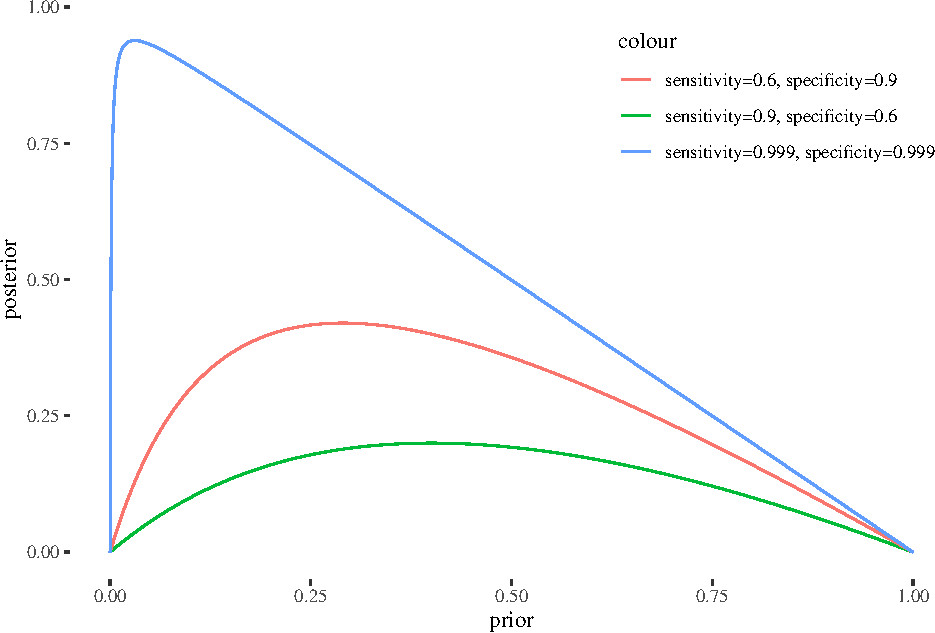
\includegraphics[width=0.9\linewidth]{conjunction-paradox_files/figure-latex/unnamed-chunk-8-1} \end{center}

\caption{The further away the posterior line from the base 
line, the stronger the evidence irrespective 
of the prior probability of the hypothesis.}
\label{fig:strength-prior-post}
\end{figure}

\begin{figure}


\begin{center}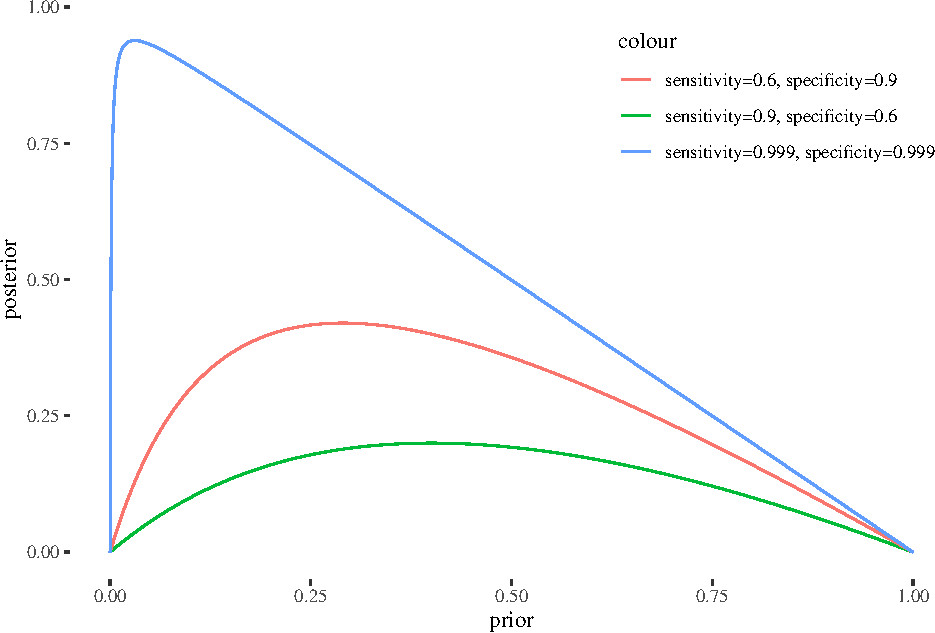
\includegraphics[width=0.9\linewidth]{conjunction-paradox_files/figure-latex/unnamed-chunk-9-1} \end{center}

\caption{Difference between priors and posteriors as a measure of te strength of evidence.}
\label{fig:strength-difference}

\end{figure}

The same approach can model the joint evidential strength of two items
of evidence, \(a \wedge b\), relative to the combined hypothesis,
\(A \wedge B\). For simplicity, assume \(a\) and \(b\) are independent
lines of evidence supporting their respective hypothesis \(A\) and
\(B\). Further, assume \(A\) and \(B\) are probabilistically independent
of the other, as in the Bayesian network in Figure
\ref{network-conjunction} (top). The graph in Figure
\ref{fig:post-indiv-joint} (top) shows how the prior probabilities are
impacted by evidence in support of a single hypothesis---say
\(a\wedge b\) supports
\(A\)\footnote{Given the assumptions of independence we are working with, the strength of $a$ in support of $A$ is the same the strength of 
$a\wedge b$ in support of $A$ since $\frac{\pr{a\wedge b \vert A}}{\pr{a \wedge b}}$ $=\frac{\pr{a \vert A}\pr{b \vert A}}{\pr{a}\pr{b}}=\frac{\pr{a \vert A}}{\pr{a}}$.}---versus
evidence in support of a joint hypothesis---say \(a\wedge b\) supports
\(A \wedge B\). The base line is lower in the latter than in the former
case because the prior probability of \(A \wedge B\) is lower than the
prior probability of \(A\). The prior of \(A\) equals \(x\) and the
prior of \(A\wedge B\) equals \(x^2\) (assuming \(A\) and \(B\) have the
same prior probability, and as noted before, are probabilistically
independent of one another).

\begin{figure}


\begin{center}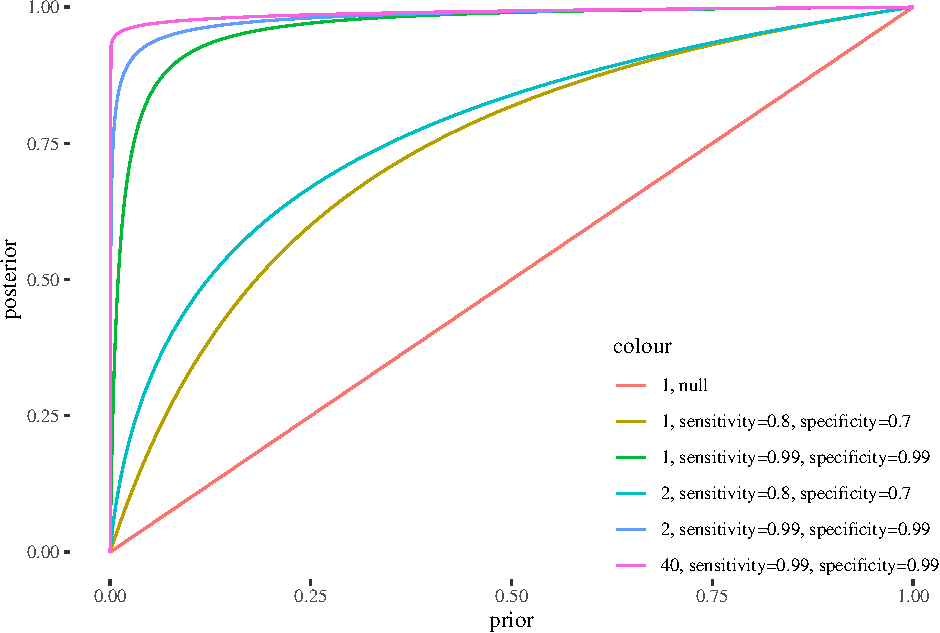
\includegraphics[width=0.9\linewidth]{conjunction-paradox_files/figure-latex/unnamed-chunk-10-1} \end{center}




\begin{center}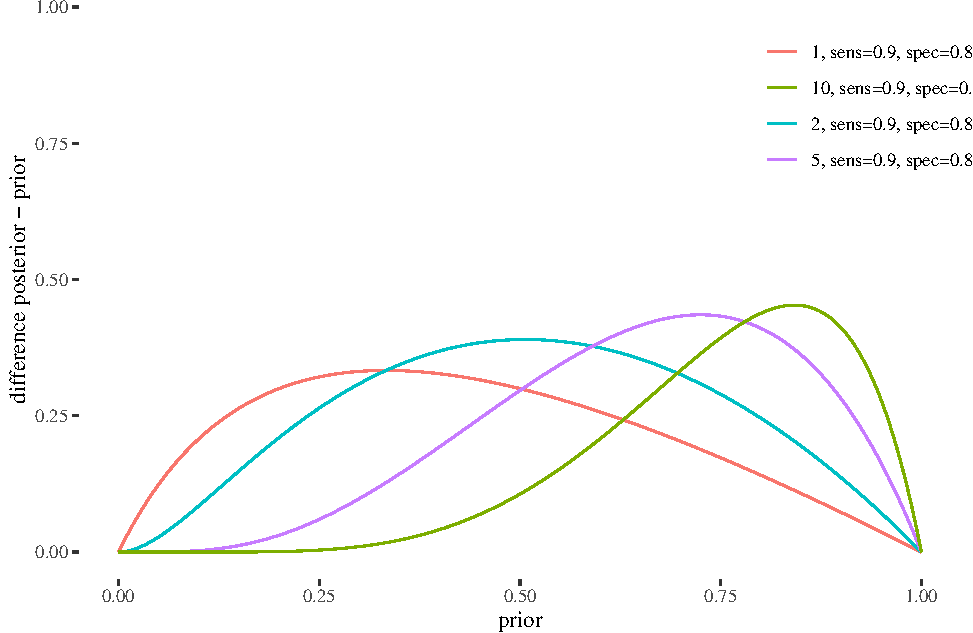
\includegraphics[width=0.9\linewidth]{conjunction-paradox_files/figure-latex/unnamed-chunk-11-1} \end{center}

\caption{The comparison is between individual support (marked by 1, for one individual 
hypothesis) and joint support (marked by 2, for a two-claim composite claim). 
Top graph: The base line for joint support ($y=x*x$) is 
below the base line for individual support ($y=x$).
Bottom graph: the two base lines are equalized and the 
posterior lines adjusted accordingly. The posterior 
lines for individual and joint support 
get closer especially for high posterior probability values.}
\label{fig:post-indiv-joint}
\end{figure}

\begin{Shaded}
\begin{Highlighting}[]
\FunctionTok{integrate}\NormalTok{(postn, }\DecValTok{0}\NormalTok{, }\DecValTok{1}\NormalTok{, }\AttributeTok{s1 =}\FloatTok{0.99}\NormalTok{ , }\AttributeTok{s2 =}\FloatTok{0.99}\NormalTok{, }\AttributeTok{n =} \DecValTok{1}\NormalTok{)}\SpecialCharTok{$}\NormalTok{val }
\end{Highlighting}
\end{Shaded}

\begin{verbatim}
## [1] 0.9628366
\end{verbatim}

\begin{Shaded}
\begin{Highlighting}[]
\FunctionTok{integrate}\NormalTok{(postn, }\DecValTok{0}\NormalTok{, }\DecValTok{1}\NormalTok{, }\AttributeTok{s1 =}\FloatTok{0.99}\NormalTok{ , }\AttributeTok{s2 =}\FloatTok{0.99}\NormalTok{, }\AttributeTok{n =} \DecValTok{2}\NormalTok{)}\SpecialCharTok{$}\NormalTok{val }
\end{Highlighting}
\end{Shaded}

\begin{verbatim}
## [1] 0.9815782
\end{verbatim}

\begin{Shaded}
\begin{Highlighting}[]
\FunctionTok{integrate}\NormalTok{(postn, }\DecValTok{0}\NormalTok{, }\DecValTok{1}\NormalTok{, }\AttributeTok{s1 =}\FloatTok{0.99}\NormalTok{ , }\AttributeTok{s2 =}\FloatTok{0.99}\NormalTok{, }\AttributeTok{n =} \DecValTok{5}\NormalTok{)}\SpecialCharTok{$}\NormalTok{val }
\end{Highlighting}
\end{Shaded}

\begin{verbatim}
## [1] 0.9876204
\end{verbatim}

\begin{Shaded}
\begin{Highlighting}[]
\FunctionTok{integrate}\NormalTok{(postn, }\DecValTok{0}\NormalTok{, }\DecValTok{1}\NormalTok{, }\AttributeTok{s1 =}\FloatTok{0.99}\NormalTok{ , }\AttributeTok{s2 =}\FloatTok{0.99}\NormalTok{, }\AttributeTok{n =} \DecValTok{10}\NormalTok{)}\SpecialCharTok{$}\NormalTok{val}
\end{Highlighting}
\end{Shaded}

\begin{verbatim}
## [1] 0.9889299
\end{verbatim}

\begin{Shaded}
\begin{Highlighting}[]
\FunctionTok{integrate}\NormalTok{(postn, }\DecValTok{0}\NormalTok{, }\DecValTok{1}\NormalTok{, }\AttributeTok{s1 =}\FloatTok{0.99}\NormalTok{ , }\AttributeTok{s2 =}\FloatTok{0.99}\NormalTok{, }\AttributeTok{n =} \DecValTok{20}\NormalTok{)}\SpecialCharTok{$}\NormalTok{val}
\end{Highlighting}
\end{Shaded}

\begin{verbatim}
## [1] 0.989491
\end{verbatim}

\begin{Shaded}
\begin{Highlighting}[]
\FunctionTok{integrate}\NormalTok{(postn, }\DecValTok{0}\NormalTok{, }\DecValTok{1}\NormalTok{, }\AttributeTok{s1 =}\FloatTok{0.5}\NormalTok{ , }\AttributeTok{s2 =}\FloatTok{0.5}\NormalTok{, }\AttributeTok{n =} \DecValTok{1}\NormalTok{)}\SpecialCharTok{$}\NormalTok{val }
\end{Highlighting}
\end{Shaded}

\begin{verbatim}
## [1] 0.5
\end{verbatim}

\begin{Shaded}
\begin{Highlighting}[]
\FunctionTok{integrate}\NormalTok{(postn, }\DecValTok{0}\NormalTok{, }\DecValTok{1}\NormalTok{, }\AttributeTok{s1 =}\FloatTok{0.5}\NormalTok{ , }\AttributeTok{s2 =}\FloatTok{0.5}\NormalTok{, }\AttributeTok{n =} \DecValTok{2}\NormalTok{)}\SpecialCharTok{$}\NormalTok{val }
\end{Highlighting}
\end{Shaded}

\begin{verbatim}
## [1] 0.5
\end{verbatim}

\begin{Shaded}
\begin{Highlighting}[]
\FunctionTok{integrate}\NormalTok{(postn, }\DecValTok{0}\NormalTok{, }\DecValTok{1}\NormalTok{, }\AttributeTok{s1 =}\FloatTok{0.5}\NormalTok{ , }\AttributeTok{s2 =}\FloatTok{0.5}\NormalTok{, }\AttributeTok{n =} \DecValTok{5}\NormalTok{)}\SpecialCharTok{$}\NormalTok{val }
\end{Highlighting}
\end{Shaded}

\begin{verbatim}
## [1] 0.5
\end{verbatim}

\begin{Shaded}
\begin{Highlighting}[]
\FunctionTok{integrate}\NormalTok{(postn, }\DecValTok{0}\NormalTok{, }\DecValTok{1}\NormalTok{, }\AttributeTok{s1 =}\FloatTok{0.5}\NormalTok{ , }\AttributeTok{s2 =}\FloatTok{0.5}\NormalTok{, }\AttributeTok{n =} \DecValTok{10}\NormalTok{)}\SpecialCharTok{$}\NormalTok{val}
\end{Highlighting}
\end{Shaded}

\begin{verbatim}
## [1] 0.5
\end{verbatim}

\begin{Shaded}
\begin{Highlighting}[]
\FunctionTok{integrate}\NormalTok{(postn, }\DecValTok{0}\NormalTok{, }\DecValTok{1}\NormalTok{, }\AttributeTok{s1 =}\FloatTok{0.5}\NormalTok{ , }\AttributeTok{s2 =}\FloatTok{0.5}\NormalTok{, }\AttributeTok{n =} \DecValTok{20}\NormalTok{)}\SpecialCharTok{$}\NormalTok{val }
\end{Highlighting}
\end{Shaded}

\begin{verbatim}
## [1] 0.5
\end{verbatim}

\begin{Shaded}
\begin{Highlighting}[]
\FunctionTok{integrate}\NormalTok{(postn, }\DecValTok{0}\NormalTok{, }\DecValTok{1}\NormalTok{, }\AttributeTok{s1 =}\FloatTok{0.99}\NormalTok{ , }\AttributeTok{s2 =}\FloatTok{0.99}\NormalTok{, }\AttributeTok{n =} \DecValTok{1}\NormalTok{)}\SpecialCharTok{$}\NormalTok{val }\SpecialCharTok{{-}} \FunctionTok{integrate}\NormalTok{(postn, }\DecValTok{0}\NormalTok{, }\DecValTok{1}\NormalTok{, }\AttributeTok{s1 =}\FloatTok{0.5}\NormalTok{ , }\AttributeTok{s2 =}\FloatTok{0.5}\NormalTok{, }\AttributeTok{n =} \DecValTok{1}\NormalTok{)}\SpecialCharTok{$}\NormalTok{val }
\end{Highlighting}
\end{Shaded}

\begin{verbatim}
## [1] 0.4628366
\end{verbatim}

\begin{Shaded}
\begin{Highlighting}[]
\FunctionTok{integrate}\NormalTok{(postn, }\DecValTok{0}\NormalTok{, }\DecValTok{1}\NormalTok{, }\AttributeTok{s1 =}\FloatTok{0.99}\NormalTok{ , }\AttributeTok{s2 =}\FloatTok{0.99}\NormalTok{, }\AttributeTok{n =} \DecValTok{2}\NormalTok{)}\SpecialCharTok{$}\NormalTok{val }\SpecialCharTok{{-}} \FunctionTok{integrate}\NormalTok{(postn, }\DecValTok{0}\NormalTok{, }\DecValTok{1}\NormalTok{, }\AttributeTok{s1 =}\FloatTok{0.5}\NormalTok{ , }\AttributeTok{s2 =}\FloatTok{0.5}\NormalTok{, }\AttributeTok{n =} \DecValTok{2}\NormalTok{)}\SpecialCharTok{$}\NormalTok{val }
\end{Highlighting}
\end{Shaded}

\begin{verbatim}
## [1] 0.4815782
\end{verbatim}

\begin{Shaded}
\begin{Highlighting}[]
\FunctionTok{integrate}\NormalTok{(postn, }\DecValTok{0}\NormalTok{, }\DecValTok{1}\NormalTok{, }\AttributeTok{s1 =}\FloatTok{0.99}\NormalTok{ , }\AttributeTok{s2 =}\FloatTok{0.99}\NormalTok{, }\AttributeTok{n =} \DecValTok{5}\NormalTok{)}\SpecialCharTok{$}\NormalTok{val }\SpecialCharTok{{-}} \FunctionTok{integrate}\NormalTok{(postn, }\DecValTok{0}\NormalTok{, }\DecValTok{1}\NormalTok{, }\AttributeTok{s1 =}\FloatTok{0.5}\NormalTok{ , }\AttributeTok{s2 =}\FloatTok{0.5}\NormalTok{, }\AttributeTok{n =} \DecValTok{5}\NormalTok{)}\SpecialCharTok{$}\NormalTok{val }
\end{Highlighting}
\end{Shaded}

\begin{verbatim}
## [1] 0.4876204
\end{verbatim}

\begin{Shaded}
\begin{Highlighting}[]
\FunctionTok{integrate}\NormalTok{(postn, }\DecValTok{0}\NormalTok{, }\DecValTok{1}\NormalTok{, }\AttributeTok{s1 =}\FloatTok{0.99}\NormalTok{ , }\AttributeTok{s2 =}\FloatTok{0.99}\NormalTok{, }\AttributeTok{n =} \DecValTok{10}\NormalTok{)}\SpecialCharTok{$}\NormalTok{val }\SpecialCharTok{{-}} \FunctionTok{integrate}\NormalTok{(postn, }\DecValTok{0}\NormalTok{, }\DecValTok{1}\NormalTok{, }\AttributeTok{s1 =}\FloatTok{0.5}\NormalTok{ , }\AttributeTok{s2 =}\FloatTok{0.5}\NormalTok{, }\AttributeTok{n =} \DecValTok{10}\NormalTok{)}\SpecialCharTok{$}\NormalTok{val }
\end{Highlighting}
\end{Shaded}

\begin{verbatim}
## [1] 0.4889299
\end{verbatim}

\begin{Shaded}
\begin{Highlighting}[]
\FunctionTok{integrate}\NormalTok{(postn, }\DecValTok{0}\NormalTok{, }\DecValTok{1}\NormalTok{, }\AttributeTok{s1 =}\FloatTok{0.99}\NormalTok{ , }\AttributeTok{s2 =}\FloatTok{0.99}\NormalTok{, }\AttributeTok{n =} \DecValTok{20}\NormalTok{)}\SpecialCharTok{$}\NormalTok{val }\SpecialCharTok{{-}} \FunctionTok{integrate}\NormalTok{(postn, }\DecValTok{0}\NormalTok{, }\DecValTok{1}\NormalTok{, }\AttributeTok{s1 =}\FloatTok{0.5}\NormalTok{ , }\AttributeTok{s2 =}\FloatTok{0.5}\NormalTok{, }\AttributeTok{n =} \DecValTok{20}\NormalTok{)}\SpecialCharTok{$}\NormalTok{val }
\end{Highlighting}
\end{Shaded}

\begin{verbatim}
## [1] 0.489491
\end{verbatim}

\begin{Shaded}
\begin{Highlighting}[]
\FunctionTok{integrate}\NormalTok{(postn, }\DecValTok{0}\NormalTok{, }\DecValTok{1}\NormalTok{, }\AttributeTok{s1 =}\FloatTok{0.99}\NormalTok{ , }\AttributeTok{s2 =}\FloatTok{0.99}\NormalTok{, }\AttributeTok{n =} \DecValTok{25}\NormalTok{)}\SpecialCharTok{$}\NormalTok{val }\SpecialCharTok{{-}} \FunctionTok{integrate}\NormalTok{(postn, }\DecValTok{0}\NormalTok{, }\DecValTok{1}\NormalTok{, }\AttributeTok{s1 =}\FloatTok{0.5}\NormalTok{ , }\AttributeTok{s2 =}\FloatTok{0.5}\NormalTok{, }\AttributeTok{n =} \DecValTok{25}\NormalTok{)}\SpecialCharTok{$}\NormalTok{val }
\end{Highlighting}
\end{Shaded}

\begin{verbatim}
## [1] 0.4895968
\end{verbatim}

\begin{Shaded}
\begin{Highlighting}[]
\FunctionTok{integrate}\NormalTok{(postn, }\DecValTok{0}\NormalTok{, }\DecValTok{1}\NormalTok{, }\AttributeTok{s1 =}\FloatTok{0.99}\NormalTok{ , }\AttributeTok{s2 =}\FloatTok{0.99}\NormalTok{, }\AttributeTok{n =} \DecValTok{40}\NormalTok{)}\SpecialCharTok{$}\NormalTok{val }\SpecialCharTok{{-}} \FunctionTok{integrate}\NormalTok{(postn, }\DecValTok{0}\NormalTok{, }\DecValTok{1}\NormalTok{, }\AttributeTok{s1 =}\FloatTok{0.5}\NormalTok{ , }\AttributeTok{s2 =}\FloatTok{0.5}\NormalTok{, }\AttributeTok{n =} \DecValTok{40}\NormalTok{)}\SpecialCharTok{$}\NormalTok{val }
\end{Highlighting}
\end{Shaded}

\begin{verbatim}
## [1] 0.4897516
\end{verbatim}

\begin{Shaded}
\begin{Highlighting}[]
\FunctionTok{integrate}\NormalTok{(postn, }\DecValTok{0}\NormalTok{, }\DecValTok{1}\NormalTok{, }\AttributeTok{s1 =}\FloatTok{0.6}\NormalTok{ , }\AttributeTok{s2 =}\FloatTok{0.7}\NormalTok{, }\AttributeTok{n =} \DecValTok{1}\NormalTok{)}\SpecialCharTok{$}\NormalTok{val }
\end{Highlighting}
\end{Shaded}

\begin{verbatim}
## [1] 0.6137056
\end{verbatim}

\begin{Shaded}
\begin{Highlighting}[]
\FunctionTok{integrate}\NormalTok{(postn, }\DecValTok{0}\NormalTok{, }\DecValTok{1}\NormalTok{, }\AttributeTok{s1 =}\FloatTok{0.6}\NormalTok{ , }\AttributeTok{s2 =}\FloatTok{0.7}\NormalTok{, }\AttributeTok{n =} \DecValTok{2}\NormalTok{)}\SpecialCharTok{$}\NormalTok{val }
\end{Highlighting}
\end{Shaded}

\begin{verbatim}
## [1] 0.6355324
\end{verbatim}

\begin{Shaded}
\begin{Highlighting}[]
\FunctionTok{integrate}\NormalTok{(postn, }\DecValTok{0}\NormalTok{, }\DecValTok{1}\NormalTok{, }\AttributeTok{s1 =}\FloatTok{0.6}\NormalTok{ , }\AttributeTok{s2 =}\FloatTok{0.7}\NormalTok{, }\AttributeTok{n =} \DecValTok{5}\NormalTok{)}\SpecialCharTok{$}\NormalTok{val }
\end{Highlighting}
\end{Shaded}

\begin{verbatim}
## [1] 0.65284
\end{verbatim}

\begin{Shaded}
\begin{Highlighting}[]
\FunctionTok{integrate}\NormalTok{(postn, }\DecValTok{0}\NormalTok{, }\DecValTok{1}\NormalTok{, }\AttributeTok{s1 =}\FloatTok{0.6}\NormalTok{ , }\AttributeTok{s2 =}\FloatTok{0.7}\NormalTok{, }\AttributeTok{n =} \DecValTok{10}\NormalTok{)}\SpecialCharTok{$}\NormalTok{val}
\end{Highlighting}
\end{Shaded}

\begin{verbatim}
## [1] 0.6595075
\end{verbatim}

\begin{Shaded}
\begin{Highlighting}[]
\FunctionTok{integrate}\NormalTok{(postn, }\DecValTok{0}\NormalTok{, }\DecValTok{1}\NormalTok{, }\AttributeTok{s1 =}\FloatTok{0.6}\NormalTok{ , }\AttributeTok{s2 =}\FloatTok{0.7}\NormalTok{, }\AttributeTok{n =} \DecValTok{20}\NormalTok{)}\SpecialCharTok{$}\NormalTok{val}
\end{Highlighting}
\end{Shaded}

\begin{verbatim}
## [1] 0.663025
\end{verbatim}

\begin{Shaded}
\begin{Highlighting}[]
\FunctionTok{integrate}\NormalTok{(postn, }\DecValTok{0}\NormalTok{, }\DecValTok{1}\NormalTok{, }\AttributeTok{s1 =}\FloatTok{0.5}\NormalTok{ , }\AttributeTok{s2 =}\FloatTok{0.5}\NormalTok{, }\AttributeTok{n =} \DecValTok{1}\NormalTok{)}\SpecialCharTok{$}\NormalTok{val }
\end{Highlighting}
\end{Shaded}

\begin{verbatim}
## [1] 0.5
\end{verbatim}

\begin{Shaded}
\begin{Highlighting}[]
\FunctionTok{integrate}\NormalTok{(postn, }\DecValTok{0}\NormalTok{, }\DecValTok{1}\NormalTok{, }\AttributeTok{s1 =}\FloatTok{0.5}\NormalTok{ , }\AttributeTok{s2 =}\FloatTok{0.5}\NormalTok{, }\AttributeTok{n =} \DecValTok{2}\NormalTok{)}\SpecialCharTok{$}\NormalTok{val }
\end{Highlighting}
\end{Shaded}

\begin{verbatim}
## [1] 0.5
\end{verbatim}

\begin{Shaded}
\begin{Highlighting}[]
\FunctionTok{integrate}\NormalTok{(postn, }\DecValTok{0}\NormalTok{, }\DecValTok{1}\NormalTok{, }\AttributeTok{s1 =}\FloatTok{0.5}\NormalTok{ , }\AttributeTok{s2 =}\FloatTok{0.5}\NormalTok{, }\AttributeTok{n =} \DecValTok{5}\NormalTok{)}\SpecialCharTok{$}\NormalTok{val }
\end{Highlighting}
\end{Shaded}

\begin{verbatim}
## [1] 0.5
\end{verbatim}

\begin{Shaded}
\begin{Highlighting}[]
\FunctionTok{integrate}\NormalTok{(postn, }\DecValTok{0}\NormalTok{, }\DecValTok{1}\NormalTok{, }\AttributeTok{s1 =}\FloatTok{0.5}\NormalTok{ , }\AttributeTok{s2 =}\FloatTok{0.5}\NormalTok{, }\AttributeTok{n =} \DecValTok{10}\NormalTok{)}\SpecialCharTok{$}\NormalTok{val}
\end{Highlighting}
\end{Shaded}

\begin{verbatim}
## [1] 0.5
\end{verbatim}

\begin{Shaded}
\begin{Highlighting}[]
\FunctionTok{integrate}\NormalTok{(postn, }\DecValTok{0}\NormalTok{, }\DecValTok{1}\NormalTok{, }\AttributeTok{s1 =}\FloatTok{0.5}\NormalTok{ , }\AttributeTok{s2 =}\FloatTok{0.5}\NormalTok{, }\AttributeTok{n =} \DecValTok{20}\NormalTok{)}\SpecialCharTok{$}\NormalTok{val }
\end{Highlighting}
\end{Shaded}

\begin{verbatim}
## [1] 0.5
\end{verbatim}

\begin{Shaded}
\begin{Highlighting}[]
\FunctionTok{integrate}\NormalTok{(postn, }\DecValTok{0}\NormalTok{, }\DecValTok{1}\NormalTok{, }\AttributeTok{s1 =}\FloatTok{0.6}\NormalTok{ , }\AttributeTok{s2 =}\FloatTok{0.7}\NormalTok{, }\AttributeTok{n =} \DecValTok{1}\NormalTok{)}\SpecialCharTok{$}\NormalTok{val }\SpecialCharTok{{-}} \FunctionTok{integrate}\NormalTok{(postn, }\DecValTok{0}\NormalTok{, }\DecValTok{1}\NormalTok{, }\AttributeTok{s1 =}\FloatTok{0.5}\NormalTok{ , }\AttributeTok{s2 =}\FloatTok{0.5}\NormalTok{, }\AttributeTok{n =} \DecValTok{1}\NormalTok{)}\SpecialCharTok{$}\NormalTok{val }
\end{Highlighting}
\end{Shaded}

\begin{verbatim}
## [1] 0.1137056
\end{verbatim}

\begin{Shaded}
\begin{Highlighting}[]
\FunctionTok{integrate}\NormalTok{(postn, }\DecValTok{0}\NormalTok{, }\DecValTok{1}\NormalTok{, }\AttributeTok{s1 =}\FloatTok{0.6}\NormalTok{ , }\AttributeTok{s2 =}\FloatTok{0.7}\NormalTok{, }\AttributeTok{n =} \DecValTok{2}\NormalTok{)}\SpecialCharTok{$}\NormalTok{val }\SpecialCharTok{{-}} \FunctionTok{integrate}\NormalTok{(postn, }\DecValTok{0}\NormalTok{, }\DecValTok{1}\NormalTok{, }\AttributeTok{s1 =}\FloatTok{0.5}\NormalTok{ , }\AttributeTok{s2 =}\FloatTok{0.5}\NormalTok{, }\AttributeTok{n =} \DecValTok{2}\NormalTok{)}\SpecialCharTok{$}\NormalTok{val }
\end{Highlighting}
\end{Shaded}

\begin{verbatim}
## [1] 0.1355324
\end{verbatim}

\begin{Shaded}
\begin{Highlighting}[]
\FunctionTok{integrate}\NormalTok{(postn, }\DecValTok{0}\NormalTok{, }\DecValTok{1}\NormalTok{, }\AttributeTok{s1 =}\FloatTok{0.6}\NormalTok{ , }\AttributeTok{s2 =}\FloatTok{0.7}\NormalTok{, }\AttributeTok{n =} \DecValTok{5}\NormalTok{)}\SpecialCharTok{$}\NormalTok{val }\SpecialCharTok{{-}} \FunctionTok{integrate}\NormalTok{(postn, }\DecValTok{0}\NormalTok{, }\DecValTok{1}\NormalTok{, }\AttributeTok{s1 =}\FloatTok{0.5}\NormalTok{ , }\AttributeTok{s2 =}\FloatTok{0.5}\NormalTok{, }\AttributeTok{n =} \DecValTok{5}\NormalTok{)}\SpecialCharTok{$}\NormalTok{val }
\end{Highlighting}
\end{Shaded}

\begin{verbatim}
## [1] 0.15284
\end{verbatim}

\begin{Shaded}
\begin{Highlighting}[]
\FunctionTok{integrate}\NormalTok{(postn, }\DecValTok{0}\NormalTok{, }\DecValTok{1}\NormalTok{, }\AttributeTok{s1 =}\FloatTok{0.6}\NormalTok{ , }\AttributeTok{s2 =}\FloatTok{0.7}\NormalTok{, }\AttributeTok{n =} \DecValTok{10}\NormalTok{)}\SpecialCharTok{$}\NormalTok{val }\SpecialCharTok{{-}} \FunctionTok{integrate}\NormalTok{(postn, }\DecValTok{0}\NormalTok{, }\DecValTok{1}\NormalTok{, }\AttributeTok{s1 =}\FloatTok{0.5}\NormalTok{ , }\AttributeTok{s2 =}\FloatTok{0.5}\NormalTok{, }\AttributeTok{n =} \DecValTok{10}\NormalTok{)}\SpecialCharTok{$}\NormalTok{val }
\end{Highlighting}
\end{Shaded}

\begin{verbatim}
## [1] 0.1595075
\end{verbatim}

\begin{Shaded}
\begin{Highlighting}[]
\FunctionTok{integrate}\NormalTok{(postn, }\DecValTok{0}\NormalTok{, }\DecValTok{1}\NormalTok{, }\AttributeTok{s1 =}\FloatTok{0.6}\NormalTok{ , }\AttributeTok{s2 =}\FloatTok{0.7}\NormalTok{, }\AttributeTok{n =} \DecValTok{20}\NormalTok{)}\SpecialCharTok{$}\NormalTok{val }\SpecialCharTok{{-}} \FunctionTok{integrate}\NormalTok{(postn, }\DecValTok{0}\NormalTok{, }\DecValTok{1}\NormalTok{, }\AttributeTok{s1 =}\FloatTok{0.5}\NormalTok{ , }\AttributeTok{s2 =}\FloatTok{0.5}\NormalTok{, }\AttributeTok{n =} \DecValTok{20}\NormalTok{)}\SpecialCharTok{$}\NormalTok{val }
\end{Highlighting}
\end{Shaded}

\begin{verbatim}
## [1] 0.163025
\end{verbatim}

\begin{Shaded}
\begin{Highlighting}[]
\FunctionTok{integrate}\NormalTok{(postn, }\DecValTok{0}\NormalTok{, }\DecValTok{1}\NormalTok{, }\AttributeTok{s1 =}\FloatTok{0.9}\NormalTok{ , }\AttributeTok{s2 =}\FloatTok{0.8}\NormalTok{, }\AttributeTok{n =} \DecValTok{1}\NormalTok{)}\SpecialCharTok{$}\NormalTok{val }
\end{Highlighting}
\end{Shaded}

\begin{verbatim}
## [1] 0.7331961
\end{verbatim}

\begin{Shaded}
\begin{Highlighting}[]
\FunctionTok{integrate}\NormalTok{(postn, }\DecValTok{0}\NormalTok{, }\DecValTok{1}\NormalTok{, }\AttributeTok{s1 =}\FloatTok{0.9}\NormalTok{ , }\AttributeTok{s2 =}\FloatTok{0.8}\NormalTok{, }\AttributeTok{n =} \DecValTok{2}\NormalTok{)}\SpecialCharTok{$}\NormalTok{val }
\end{Highlighting}
\end{Shaded}

\begin{verbatim}
## [1] 0.7717311
\end{verbatim}

\begin{Shaded}
\begin{Highlighting}[]
\FunctionTok{integrate}\NormalTok{(postn, }\DecValTok{0}\NormalTok{, }\DecValTok{1}\NormalTok{, }\AttributeTok{s1 =}\FloatTok{0.9}\NormalTok{ , }\AttributeTok{s2 =}\FloatTok{0.8}\NormalTok{, }\AttributeTok{n =} \DecValTok{5}\NormalTok{)}\SpecialCharTok{$}\NormalTok{val }
\end{Highlighting}
\end{Shaded}

\begin{verbatim}
## [1] 0.7990992
\end{verbatim}

\begin{Shaded}
\begin{Highlighting}[]
\FunctionTok{integrate}\NormalTok{(postn, }\DecValTok{0}\NormalTok{, }\DecValTok{1}\NormalTok{, }\AttributeTok{s1 =}\FloatTok{0.9}\NormalTok{ , }\AttributeTok{s2 =}\FloatTok{0.8}\NormalTok{, }\AttributeTok{n =} \DecValTok{10}\NormalTok{)}\SpecialCharTok{$}\NormalTok{val}
\end{Highlighting}
\end{Shaded}

\begin{verbatim}
## [1] 0.8086466
\end{verbatim}

\begin{Shaded}
\begin{Highlighting}[]
\FunctionTok{integrate}\NormalTok{(postn, }\DecValTok{0}\NormalTok{, }\DecValTok{1}\NormalTok{, }\AttributeTok{s1 =}\FloatTok{0.9}\NormalTok{ , }\AttributeTok{s2 =}\FloatTok{0.8}\NormalTok{, }\AttributeTok{n =} \DecValTok{20}\NormalTok{)}\SpecialCharTok{$}\NormalTok{val}
\end{Highlighting}
\end{Shaded}

\begin{verbatim}
## [1] 0.8134273
\end{verbatim}

\begin{Shaded}
\begin{Highlighting}[]
\FunctionTok{integrate}\NormalTok{(postn, }\DecValTok{0}\NormalTok{, }\DecValTok{1}\NormalTok{, }\AttributeTok{s1 =}\FloatTok{0.5}\NormalTok{ , }\AttributeTok{s2 =}\FloatTok{0.5}\NormalTok{, }\AttributeTok{n =} \DecValTok{1}\NormalTok{)}\SpecialCharTok{$}\NormalTok{val }
\end{Highlighting}
\end{Shaded}

\begin{verbatim}
## [1] 0.5
\end{verbatim}

\begin{Shaded}
\begin{Highlighting}[]
\FunctionTok{integrate}\NormalTok{(postn, }\DecValTok{0}\NormalTok{, }\DecValTok{1}\NormalTok{, }\AttributeTok{s1 =}\FloatTok{0.5}\NormalTok{ , }\AttributeTok{s2 =}\FloatTok{0.5}\NormalTok{, }\AttributeTok{n =} \DecValTok{2}\NormalTok{)}\SpecialCharTok{$}\NormalTok{val }
\end{Highlighting}
\end{Shaded}

\begin{verbatim}
## [1] 0.5
\end{verbatim}

\begin{Shaded}
\begin{Highlighting}[]
\FunctionTok{integrate}\NormalTok{(postn, }\DecValTok{0}\NormalTok{, }\DecValTok{1}\NormalTok{, }\AttributeTok{s1 =}\FloatTok{0.5}\NormalTok{ , }\AttributeTok{s2 =}\FloatTok{0.5}\NormalTok{, }\AttributeTok{n =} \DecValTok{5}\NormalTok{)}\SpecialCharTok{$}\NormalTok{val }
\end{Highlighting}
\end{Shaded}

\begin{verbatim}
## [1] 0.5
\end{verbatim}

\begin{Shaded}
\begin{Highlighting}[]
\FunctionTok{integrate}\NormalTok{(postn, }\DecValTok{0}\NormalTok{, }\DecValTok{1}\NormalTok{, }\AttributeTok{s1 =}\FloatTok{0.5}\NormalTok{ , }\AttributeTok{s2 =}\FloatTok{0.5}\NormalTok{, }\AttributeTok{n =} \DecValTok{10}\NormalTok{)}\SpecialCharTok{$}\NormalTok{val}
\end{Highlighting}
\end{Shaded}

\begin{verbatim}
## [1] 0.5
\end{verbatim}

\begin{Shaded}
\begin{Highlighting}[]
\FunctionTok{integrate}\NormalTok{(postn, }\DecValTok{0}\NormalTok{, }\DecValTok{1}\NormalTok{, }\AttributeTok{s1 =}\FloatTok{0.5}\NormalTok{ , }\AttributeTok{s2 =}\FloatTok{0.5}\NormalTok{, }\AttributeTok{n =} \DecValTok{20}\NormalTok{)}\SpecialCharTok{$}\NormalTok{val }
\end{Highlighting}
\end{Shaded}

\begin{verbatim}
## [1] 0.5
\end{verbatim}

\begin{Shaded}
\begin{Highlighting}[]
\FunctionTok{integrate}\NormalTok{(postn, }\DecValTok{0}\NormalTok{, }\DecValTok{1}\NormalTok{, }\AttributeTok{s1 =}\FloatTok{0.9}\NormalTok{ , }\AttributeTok{s2 =}\FloatTok{0.8}\NormalTok{, }\AttributeTok{n =} \DecValTok{1}\NormalTok{)}\SpecialCharTok{$}\NormalTok{val }\SpecialCharTok{{-}} \FunctionTok{integrate}\NormalTok{(postn, }\DecValTok{0}\NormalTok{, }\DecValTok{1}\NormalTok{, }\AttributeTok{s1 =}\FloatTok{0.5}\NormalTok{ , }\AttributeTok{s2 =}\FloatTok{0.5}\NormalTok{, }\AttributeTok{n =} \DecValTok{1}\NormalTok{)}\SpecialCharTok{$}\NormalTok{val }
\end{Highlighting}
\end{Shaded}

\begin{verbatim}
## [1] 0.2331961
\end{verbatim}

\begin{Shaded}
\begin{Highlighting}[]
\FunctionTok{integrate}\NormalTok{(postn, }\DecValTok{0}\NormalTok{, }\DecValTok{1}\NormalTok{, }\AttributeTok{s1 =}\FloatTok{0.9}\NormalTok{ , }\AttributeTok{s2 =}\FloatTok{0.8}\NormalTok{, }\AttributeTok{n =} \DecValTok{2}\NormalTok{)}\SpecialCharTok{$}\NormalTok{val }\SpecialCharTok{{-}} \FunctionTok{integrate}\NormalTok{(postn, }\DecValTok{0}\NormalTok{, }\DecValTok{1}\NormalTok{, }\AttributeTok{s1 =}\FloatTok{0.5}\NormalTok{ , }\AttributeTok{s2 =}\FloatTok{0.5}\NormalTok{, }\AttributeTok{n =} \DecValTok{2}\NormalTok{)}\SpecialCharTok{$}\NormalTok{val }
\end{Highlighting}
\end{Shaded}

\begin{verbatim}
## [1] 0.2717311
\end{verbatim}

\begin{Shaded}
\begin{Highlighting}[]
\FunctionTok{integrate}\NormalTok{(postn, }\DecValTok{0}\NormalTok{, }\DecValTok{1}\NormalTok{, }\AttributeTok{s1 =}\FloatTok{0.9}\NormalTok{ , }\AttributeTok{s2 =}\FloatTok{0.8}\NormalTok{, }\AttributeTok{n =} \DecValTok{5}\NormalTok{)}\SpecialCharTok{$}\NormalTok{val }\SpecialCharTok{{-}} \FunctionTok{integrate}\NormalTok{(postn, }\DecValTok{0}\NormalTok{, }\DecValTok{1}\NormalTok{, }\AttributeTok{s1 =}\FloatTok{0.5}\NormalTok{ , }\AttributeTok{s2 =}\FloatTok{0.5}\NormalTok{, }\AttributeTok{n =} \DecValTok{5}\NormalTok{)}\SpecialCharTok{$}\NormalTok{val }
\end{Highlighting}
\end{Shaded}

\begin{verbatim}
## [1] 0.2990992
\end{verbatim}

\begin{Shaded}
\begin{Highlighting}[]
\FunctionTok{integrate}\NormalTok{(postn, }\DecValTok{0}\NormalTok{, }\DecValTok{1}\NormalTok{, }\AttributeTok{s1 =}\FloatTok{0.9}\NormalTok{ , }\AttributeTok{s2 =}\FloatTok{0.8}\NormalTok{, }\AttributeTok{n =} \DecValTok{10}\NormalTok{)}\SpecialCharTok{$}\NormalTok{val }\SpecialCharTok{{-}} \FunctionTok{integrate}\NormalTok{(postn, }\DecValTok{0}\NormalTok{, }\DecValTok{1}\NormalTok{, }\AttributeTok{s1 =}\FloatTok{0.5}\NormalTok{ , }\AttributeTok{s2 =}\FloatTok{0.5}\NormalTok{, }\AttributeTok{n =} \DecValTok{10}\NormalTok{)}\SpecialCharTok{$}\NormalTok{val }
\end{Highlighting}
\end{Shaded}

\begin{verbatim}
## [1] 0.3086466
\end{verbatim}

\begin{Shaded}
\begin{Highlighting}[]
\FunctionTok{integrate}\NormalTok{(postn, }\DecValTok{0}\NormalTok{, }\DecValTok{1}\NormalTok{, }\AttributeTok{s1 =}\FloatTok{0.9}\NormalTok{ , }\AttributeTok{s2 =}\FloatTok{0.8}\NormalTok{, }\AttributeTok{n =} \DecValTok{20}\NormalTok{)}\SpecialCharTok{$}\NormalTok{val }\SpecialCharTok{{-}} \FunctionTok{integrate}\NormalTok{(postn, }\DecValTok{0}\NormalTok{, }\DecValTok{1}\NormalTok{, }\AttributeTok{s1 =}\FloatTok{0.5}\NormalTok{ , }\AttributeTok{s2 =}\FloatTok{0.5}\NormalTok{, }\AttributeTok{n =} \DecValTok{20}\NormalTok{)}\SpecialCharTok{$}\NormalTok{val }
\end{Highlighting}
\end{Shaded}

\begin{verbatim}
## [1] 0.3134273
\end{verbatim}

\begin{Shaded}
\begin{Highlighting}[]
\FunctionTok{integrate}\NormalTok{(post, }\DecValTok{0}\NormalTok{, }\DecValTok{1}\NormalTok{, }\AttributeTok{s1 =}\FloatTok{0.99}\NormalTok{ , }\AttributeTok{s2 =}\FloatTok{0.99}\NormalTok{)}\SpecialCharTok{$}\NormalTok{val }
\end{Highlighting}
\end{Shaded}

\begin{verbatim}
## [1] 0.9628366
\end{verbatim}

\begin{Shaded}
\begin{Highlighting}[]
\FunctionTok{integrate}\NormalTok{(postn, }\DecValTok{0}\NormalTok{, }\DecValTok{1}\NormalTok{, }\AttributeTok{s1 =}\FloatTok{0.99}\NormalTok{ , }\AttributeTok{s2 =}\FloatTok{0.99}\NormalTok{ , }\AttributeTok{n =} \DecValTok{2}\NormalTok{)}\SpecialCharTok{$}\NormalTok{val}
\end{Highlighting}
\end{Shaded}

\begin{verbatim}
## [1] 0.9815782
\end{verbatim}

\begin{Shaded}
\begin{Highlighting}[]
\FunctionTok{integrate}\NormalTok{(postn, }\DecValTok{0}\NormalTok{, }\DecValTok{1}\NormalTok{, }\AttributeTok{s1 =}\FloatTok{0.99}\NormalTok{ , }\AttributeTok{s2 =}\FloatTok{0.99}\NormalTok{ , }\AttributeTok{n =} \DecValTok{5}\NormalTok{)}\SpecialCharTok{$}\NormalTok{val}
\end{Highlighting}
\end{Shaded}

\begin{verbatim}
## [1] 0.9876204
\end{verbatim}

\begin{figure}


\begin{center}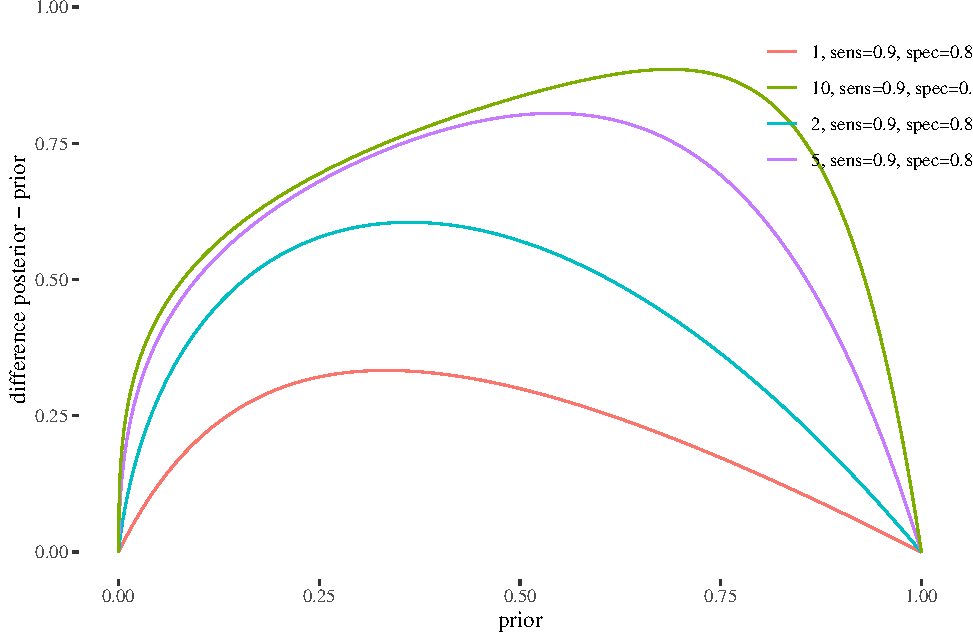
\includegraphics[width=0.9\linewidth]{conjunction-paradox_files/figure-latex/unnamed-chunk-16-1} \end{center}


\end{figure}

\begin{Shaded}
\begin{Highlighting}[]
\NormalTok{prior\_a }\OtherTok{\textless{}{-}} \FloatTok{0.6}
\NormalTok{prior\_b }\OtherTok{\textless{}{-}} \FloatTok{0.4}
\NormalTok{sen\_a }\OtherTok{\textless{}{-}} \FloatTok{0.85}  \CommentTok{\# Pr(a given A)}
\NormalTok{spe\_a }\OtherTok{\textless{}{-}} \FloatTok{0.75}  \CommentTok{\#  Pr(not{-}a given not{-}A)}
\NormalTok{sen\_b }\OtherTok{\textless{}{-}} \FloatTok{0.7}
\NormalTok{spe\_b }\OtherTok{\textless{}{-}} \FloatTok{0.75}

\NormalTok{prior\_ab }\OtherTok{\textless{}{-}}\NormalTok{ prior\_a}\SpecialCharTok{*}\NormalTok{prior\_b }

\NormalTok{bf\_a }\OtherTok{\textless{}{-}}\NormalTok{ sen\_a}\SpecialCharTok{/}\NormalTok{((sen\_a}\SpecialCharTok{*}\NormalTok{prior\_a)}\SpecialCharTok{+}\NormalTok{((}\DecValTok{1}\SpecialCharTok{{-}}\NormalTok{spe\_a)}\SpecialCharTok{*}\NormalTok{(}\DecValTok{1}\SpecialCharTok{{-}}\NormalTok{prior\_a)))}
\NormalTok{bf\_b }\OtherTok{\textless{}{-}}\NormalTok{ sen\_b}\SpecialCharTok{/}\NormalTok{((sen\_b}\SpecialCharTok{*}\NormalTok{prior\_b)}\SpecialCharTok{+}\NormalTok{((}\DecValTok{1}\SpecialCharTok{{-}}\NormalTok{spe\_b)}\SpecialCharTok{*}\NormalTok{(}\DecValTok{1}\SpecialCharTok{{-}}\NormalTok{prior\_b)))}
\NormalTok{bf\_ab }\OtherTok{\textless{}{-}}\NormalTok{ bf\_a}\SpecialCharTok{*}\NormalTok{bf\_b}

\NormalTok{post\_a }\OtherTok{\textless{}{-}}\NormalTok{ bf\_a}\SpecialCharTok{*}\NormalTok{prior\_a}
\NormalTok{post\_b }\OtherTok{\textless{}{-}}\NormalTok{ bf\_b}\SpecialCharTok{*}\NormalTok{prior\_b}
\NormalTok{post\_ab }\OtherTok{\textless{}{-}}\NormalTok{ bf\_ab}\SpecialCharTok{*}\NormalTok{prior\_ab}

\NormalTok{prior\_a}
\end{Highlighting}
\end{Shaded}

\begin{verbatim}
## [1] 0.6
\end{verbatim}

\begin{Shaded}
\begin{Highlighting}[]
\NormalTok{prior\_b}
\end{Highlighting}
\end{Shaded}

\begin{verbatim}
## [1] 0.4
\end{verbatim}

\begin{Shaded}
\begin{Highlighting}[]
\NormalTok{prior\_ab}
\end{Highlighting}
\end{Shaded}

\begin{verbatim}
## [1] 0.24
\end{verbatim}

\begin{Shaded}
\begin{Highlighting}[]
\NormalTok{post\_a}
\end{Highlighting}
\end{Shaded}

\begin{verbatim}
## [1] 0.8360656
\end{verbatim}

\begin{Shaded}
\begin{Highlighting}[]
\NormalTok{post\_b}
\end{Highlighting}
\end{Shaded}

\begin{verbatim}
## [1] 0.6511628
\end{verbatim}

\begin{Shaded}
\begin{Highlighting}[]
\NormalTok{post\_ab}
\end{Highlighting}
\end{Shaded}

\begin{verbatim}
## [1] 0.5444148
\end{verbatim}

\begin{Shaded}
\begin{Highlighting}[]
\NormalTok{prior\_a }\OtherTok{\textless{}{-}} \FloatTok{0.24}
\NormalTok{prior\_b }\OtherTok{\textless{}{-}} \FloatTok{0.24}

\NormalTok{bf\_a }\OtherTok{\textless{}{-}}\NormalTok{ sen\_a}\SpecialCharTok{/}\NormalTok{((sen\_a}\SpecialCharTok{*}\NormalTok{prior\_a)}\SpecialCharTok{+}\NormalTok{((}\DecValTok{1}\SpecialCharTok{{-}}\NormalTok{spe\_a)}\SpecialCharTok{*}\NormalTok{(}\DecValTok{1}\SpecialCharTok{{-}}\NormalTok{prior\_a)))}
\NormalTok{bf\_b }\OtherTok{\textless{}{-}}\NormalTok{ sen\_b}\SpecialCharTok{/}\NormalTok{((sen\_b}\SpecialCharTok{*}\NormalTok{prior\_b)}\SpecialCharTok{+}\NormalTok{((}\DecValTok{1}\SpecialCharTok{{-}}\NormalTok{spe\_b)}\SpecialCharTok{*}\NormalTok{(}\DecValTok{1}\SpecialCharTok{{-}}\NormalTok{prior\_b)))}
\NormalTok{bf\_ab }\OtherTok{\textless{}{-}}\NormalTok{ bf\_a}\SpecialCharTok{*}\NormalTok{bf\_b}

\NormalTok{post\_a }\OtherTok{\textless{}{-}}\NormalTok{ bf\_a}\SpecialCharTok{*}\NormalTok{prior\_a}
\NormalTok{post\_b }\OtherTok{\textless{}{-}}\NormalTok{ bf\_b}\SpecialCharTok{*}\NormalTok{prior\_b}
\NormalTok{post\_a}
\end{Highlighting}
\end{Shaded}

\begin{verbatim}
## [1] 0.5177665
\end{verbatim}

\begin{Shaded}
\begin{Highlighting}[]
\NormalTok{post\_b}
\end{Highlighting}
\end{Shaded}

\begin{verbatim}
## [1] 0.4692737
\end{verbatim}

What happens if we make the same comparison between individual and
composite claims by equalizing their prior probability? If the claims
are independent and equiprobable, let \(x\) be the prior probability of
an individual claim (when it is considered in isolation) and let
\(x^{1/k}\) the prior probability of the same individual claim when it
is part of a composite claim that consists of \(k\) claims. In this
way---and again, assuming independence and equiprobability of the
hypotheses---the prior probability of the composite claim equals the
prior probability of the individual claim since \((x^{1/k})^k=x\), as
desired. These different claims are then plotted having the same priors.
Here we are explicitly factoring out the role of prior probabilities.
Figure \ref{fig:post-indiv-joint} (bottom) shows the result of this
process of equalization.

We observe two things. First, the difference in posterior probability,
though still present, is less significant, especially for values above
the 75\% threshold and even more clearly above the 95\% threshold.
Second, whatever remaining difference in posterior probability is now
reversed, that is, a composite claim supported by several items of
evidence has a higher posterior probability compared to an individual
claim supported by one item of evidence. This second observation agrees
with the analysis based on the Bayes factor and the likelihood ratio in
the earlier section. That analysis showed that the support for a
composite claim by a joint body of evidence often exceeds the support
for an individual claim.

These two observations establish that, by factorig out prior
probabilities and under certain independence assumptions, whenever the
individual claims meet the applicable posterior threhsold, so does the
composite claim. This verifies aggregation. Conversely, whenever the
composite claim, say \(A \wedge B\), meets the applicable posterior
threshold, so do the individual claims insofar as the threshold is about
75\% or higher. This verifies---to some approximation and in a limited
class of cases---the other direction of the conjunction principle, what
we called distribution.

Has the distribution paradox been eliminated then? The approach we have
just described---equalizing the prior probabilities across individual
and composite claims---does not entirely eliminate the paradox. There
are still cases in which a composite hypothesis, say \(A \wedge B\),
receives stronger support than an individual hypothesis, given the same
body of evidence. Sensitivity to priors seems to play a role. But it
cannot be the only factor at play, or else the equalization of the prior
probabilities would have eliminated the paradox entirely. So what else
is going on?

\hypertarget{weaker-claims-weaken-sensitivity}{%
\subsection{Weaker Claims Weaken
Sensitivity}\label{weaker-claims-weaken-sensitivity}}

Let's examine more closely the Bayes factor and the likelihood ratio as
measures of evidential strength. Likelihood ratios are comparative in
nature. Suppose we compare claim \(A\) and claim \(A\wedge B\) relative
to the same body of evidence \(a\wedge b\). Thinks of \(A\) as `the
defendant physically injured the victim' while \(B\) as `the defendant
knew the victim was a firefighter.' Think of \(a\) and \(b\) as
testimonies each supporting one of the two hypotheses. We are still
working with the Bayesian networks in Figure \ref{network-conjunction}.

Consider the combined body of evidence \(a\wedge b\). Which claim
between \(A\) and \(A\wedge B\) will receive more support by evidence
\(a\wedge b\)? Intuitively, one might think that \(A\) should receive
more or at least equal support compared to \(A\wedge B\) . After all,
\(A\wedge B\) is a stronger claim than \(A\) and thus more difficult to
establish than \(A\), other things being equal. In terms of posterior
probabilities, this is true. The posterior probability of \(A\wedge B\)
should not be higher than the posterior probability of \(A\) alone given
evidence \(a \wedge b\).

Let's now think in terms of evidential support. Formally, the question
is whether
\(\frac{\pr{a\wedge b \vert A}}{\pr{a\wedge b \vert A \wedge B}}\) is
less than one or greater than one. Given the customary independencies
between evidence and hypotheses,

\[\frac{\pr{a\wedge b \vert A}}{\pr{a\wedge b \vert A \wedge B}}=\frac{\pr{a \vert A} \pr{b \vert A}}{\pr{a \vert A} \pr{b \vert B}}=\frac{\pr{b \vert A}}{\pr{b \vert B}}<1.\]

\noindent The reason is that \(\pr{b \vert A} < \pr{b \vert B}\) since
the sensitivity of \(b\) relative to \(B\) should be higher than the
sensitivity of \(b\) relative to \(A\).\footnote{GIVE PROOF OF THIS}
This is obvious if \(A\) and \(b\) are independent claims, as in the
Bayesian networks in Figure \ref{network-conjunction} (bottom). In this
case, \(\pr{b \vert A}=\pr{b}\).\\
So \(\frac{\pr{b}}{\pr{b \vert B}}<1\) since \(b\), by assumption,
positively supports \(B\), or in other words,
\(\frac{\pr{b \vert B}}{\pr{b}}>1\). Thus, \(a\wedge b\) supports
\(A\wedge B\) more than it supports \(A\) alone. This is not what one
would expect intuitively.

The same conslusion holds using the Bayes factor. If
\(\frac{\pr{a\wedge b \vert A}}{\pr{a\wedge b \vert A \wedge B}}<1\),
then

\[\frac{\pr{a\wedge b \vert A}}{\pr{a\wedge b}} < \frac{\pr{a\wedge b \vert A \wedge B}}{\pr{a\wedge b}}   \]

\noindent Thus, evidence \(a\wedge b\) better supports, even on an
absolute scale, \(A \wedge B\) compared to \(A\). Note that, even if the
Baye factor depends on the priors, the difference here is not due to the
difference between the priors of \(A\) and the priors of \(A\wedge B\)
since the denominator is simply
\(\pr{a\wedge b}\).\footnote{Note that $\pr{a\wedge b \vert A}\pr{A}+ \pr{a\wedge b \vert \neg A}\pr\neg {A}$ is the same as $\pr{a\wedge b \vert (A\wedge B)}\pr{A\wedge B}+ \pr{a\wedge b \vert \neg (A\wedge B)}\pr{\neg (A\wedge B)}$. \textbf{NEED A PROOF FOR THIS BUT IT SHOULD HOLD, RIGHT?}}

What we have said so far agrees with the claim defended in the previous
section. That is, even when \(a\wedge b\) strongly supports
\(A \wedge B\), the same evidence need \textit{not} strongly support
\(A\). Formally,

\[\frac{\pr{a\wedge b \vert A}}{\pr{a\wedge b \vert \neg A}} < \frac{\pr{a\wedge b \vert A \wedge B}}{\pr{a\wedge b \vert \neg (A \wedge B)}}\]

\noindent In other words, even if \(a\wedge b\) favors \(A\wedge B\)
over its negation to a very high degree, it need not favor equally
strongly \(A\) over its negation. This is a comparative claim about two
compartive claims, and as such, it may not be easy to parse. Evidential
support, when it is formalized by the likelihoo ratio, is always
relative to a contrast class. In comparing the support that the same
body of evidence provides to \(A\) as contrasted to \(A\wedge B\), it
might be better to include these two hypotheses in the contrast class.
So the expression
\(\frac{\pr{a\wedge b \vert A}}{\pr{a\wedge b \vert A \wedge B}}\) is
more straightforward.

No matter the formulation, the same conclusion holds. Evidence
\(a\wedge b\) supports the composite claim \(A\wedge B\) more than it
supports the weaker claim \(A\), even assuming that \(A\) and \(B\) are
independent of one another and thus not mutually reinforcing. This
conclusion seems paradoxical. How should we make sense of it? At first,
we thought the paradox could be due to prior dependency since the
combined likelihood ratio
\(\frac{\pr{a\wedge b \vert A \wedge B}}{\pr{a\wedge b \vert \neg (A \wedge B)}}\)
varies depending on the priors of \(A\) and \(B\). But this argument
seems to no longer holds since in case of
\(\frac{\pr{a\wedge b \vert A}}{\pr{a\wedge b \vert A \wedge B}}\) any
prior dependency seems to have been eliminated. After all, if
\(\frac{\pr{a\wedge b \vert A}}{\pr{a\wedge b \vert A \wedge B}}<1\),
the sensitivity of \(a\wedge b\) must be worse relative to \(A\) than
the composite claim \(A \wedge B\).

Sensitivity is a crucial property of the quality of the evidence.
Everything else being equal, the lower the sensitivity of the evidence,
the lower its evidential strength. The importance of sensitivity as a
factor for assessing the strength of the evidence is hard to dispute. So
why is the sensitivity of \(a\wedge b\) worse relative to \(A\) than
\(A \wedge B\)? Suppose \(A\) is the case. If \(A\) is the case, in
order for \(a\wedge b\) to arise, both \(a\) and \(b\) should pick up on
\(A\). If \(b\) fails to pick up on \(A\), then \(A \wedge b\) would not
arise even if \(a\) pick up on
\(A\).\footnote{The occurrance of $a\wedge b$ is less likely to occur than just $a$ alone picking up on $A$ because $b$ may fail---and fail more often than $a$ would---in picking up on $A$.}
Suppose instead \(A\wedge B\) holds. In this case, \(a\wedge b\) would
arise even if \(b\) fails to pick up on \(A\) so long \(a\) picks up on
\(A\) and \(b\) picks up on \(B\). Now of course \(b\) could also fail
to pick on \(B\) just like \(a\) could fail to pick up on \(B\). But we
are assuming that \(b\) is better than \(a\) at tracking \(B\). So \(b\)
will fail less often than \(a\) at picking up on \(B\). Thus, the
sensitivity of \(a\wedge b\) relative to \(A\wedge B\) is better than
the sensitivity of \(a\) relative to \(A\) alone. This is a subtle point
that probability theory helps to bring out clearly.

How big are these variations?
\textbf{PLOT GRAPH TO GET A SENSE OF VARIATIONS OF SENSITIVITY}

One explanation of the paradox, then, is the difference in sensitivity.
The sensitivity of \(a\wedge b\) relative to \(A\wedge B\) is better
than the sensitivity of the same evidence relative to \(A\).
Consequently, other thigns being equal, evidence \(a\wedge b\) supports
\(A\wedge B\) better than \(A\). However counterintuitive this might
seem, we should accept this fact and admit that our intuitions were
wrong. So the fallacy seems to be to assume that the sensitivity of
\(a\wedge b\) relative to \(A\) cannot be lower than the senstivity of
\(a\wedge b\) relative to \(A\wedge B\). The thought would be something
like this: if \(a \wedge b\) tracks \(A\wedge B\) to some degree, it
surely must be able to track \(A\) alone, at least as well. But we have
just shown that we cannot assume that
\(\pr{a\wedge b \vert A} \geq \pr{a\wedge b \vert A\wedge B}\) and in
fact the opposite is the case,
\(\pr{a\wedge b \vert A} < \pr{a\wedge b \vert A\wedge B}\).

Another way to convince ourselves this is the case is to run a
simulation. Suppose we are deciding about the truth of \(A\) and the the
truth of \(A\wedge B\), and we have a fixed body of evidence, say,
\(a\wedge b\) that speaks in favor of both claims.
\todo{M: Run simulation to show that same diagnostic test for composite claim would perform better then when applied to individual claim (worse LR). How do to do this? HELP!}

We should circumscribe the point we just made since it does not always
hold. Suppose, as in Figure \ref{network-unrelated}, that \(H\) is a
claim unrelated to \(A\) and evidence \(a\). Evidence \(a\) supports
\(A\). Would the composite claim \(A\wedge H\) be better supported by
\(a\) than \(A\) alone? It would not. Mere tagging an unrelated
hypothesis does not strengthen the evidence. Note that
\(\pr{a \vert A}=\pr{a \vert A \wedge H}\) because \(H\) is indepedent
from everything else. Thus,

\[\frac{\pr{a \vert A}}{\pr{a \vert A \wedge H}}=\frac{\pr{a \vert A}}{\pr{a \vert A}}=1.\]

\noindent Tagging an unrelated claim \(H\) does not strengthen the
evidence, but leaves it unchanged. Similarly, suppose \(B\) constitutes
one element of a crime and \(A\) constitutes the other element. The two
claims are independent, each supported by items of evidence \(a\) and
\(b\) respectively. This is our standard set up. If \(a\) supports
\(A\), would \(a\) support \(A\wedge B\) more strongly than it supports
\(A\) alone? Here we no longer have \(a\wedge b\), but instead, \(a\)
alone. The question is whether
\(\frac{\pr{a \vert A}}{\pr{a \vert A \wedge B}}>1\) or
\(\frac{\pr{a \vert A}}{\pr{a \vert A \wedge B}}<1\). Given the usual
independencies between evidence and hypotheses,

\[\frac{\pr{a\vert A}}{\pr{a \vert A \wedge B}}=\frac{\pr{a \vert A}}{\pr{a \vert A}}=1\]

Evidence \(a\) supports \(A\) and \(A\wedge B\) to the same extent. One
might complain that this is counterintuitive. How can it be that \(a\)
supports \(A\) to the same degree that it supports the more demanding
claim \(A\wedge H\) or \(A\wedge B\)? For suppose we have evidence \(a\)
in favor of \(A\) and then wonder whether we could use that evidence in
support of another claim \(H\) or \(B\). By tagging \(H\) or \(B\) to
\(A\), we can at least say that we have evidence \(a\) for \(A\wedge H\)
or \(A\wedge B\) that is at least as strong as evidence \(a\) in support
of \(A\). But note that \(\frac{\pr{a \vert A}}{\pr{a\vert neg A}}>1\)
even though \(\frac{\pr{a \vert H}}{\pr{a\vert neg H}=1}\) and
\(\frac{\pr{a \vert B}}{\pr{a\vert neg B}=1}\) (assuming \(A\) and \(B\)
are independent). So \(a\) does not support \(H\) or \(B\) to the same
degree that it supports \(A\). However, \(a\) supports \(A\) to the same
degree that it supports \(A\wedge H\) or \(A\wedge B\).

What should we make of this? The commonality between \(H\) and \(B\) is
that they are irrelevant for \(a\). Evidence \(a\) does not increase nor
decrease their probability so the evidence is irrelevant for them. So
the upshot here is that, tagging an irrelevant hypothesis does not
change evidential support. The other upshot is that tagging a relevant
hypothesis---a hypthesis that does bear on the evidence in one way or
another, such as \(B\) relative to \(a\wedge b\)---does increase
evidential support.
\todo{M: How to explain this better? Can we make this plausible? HELP!}

\begin{center}
\begin{figure}[h!]
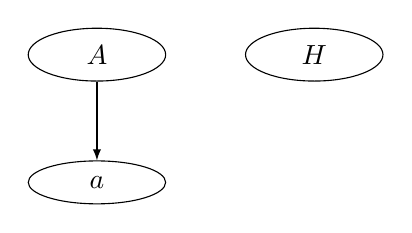
\begin{tikzpicture}[
  node distance=1cm and 1cm,
  mynode/.style={draw,ellipse,text width=1cm,align=center}
]
\node[mynode] (h1) {$A$};
\node[mynode, right =of h1] (h) {$H$};
\node[mynode, below  =of h1] (e1) {$a$};
\path 
(h1) edge[-latex] (e1);
\end{tikzpicture}

\caption{Bayesian network with wholly unrelated claim $H$.}
\label{network-unrelated}
\end{figure}
\end{center}

The intuition that the same evidence tracks the conjunction
\(A\wedge B\) better than one of the conjuncts \(A\) and \(B\) might
rest on another model of what is going on. Say \(ab\) is an item of
evidence that arises when \(A\) or \(B\) occurs with \(60\%\)
probability. That is, \(\pr{ab \vert A}=\pr{a \vert B}=60\%\). What
would be the sensitivity of \(ab\) relative to the conjunction
\(A\wedge B\), \(\pr{ab \vert A\wedge B}\)? We can represent this set up
in Figure \ref{network-ab}. Intuitvely, one might reason as follows.
There are two paths leading to \(ab\), one path starts with \(A\) and
another path starts with \(B\). When both these pathst are active, since
we are assuming \(A\wedge B\), then the probability of \(ab\) must be
higher than if just one of the two paths is active. Hence,
\(\pr{ab \vert A\wedge B}\geq 60\%\).
\todo{M: Is this true probabilistically? If not, what assumptions are required? HELP!}

\begin{center}
\begin{figure}[h!]
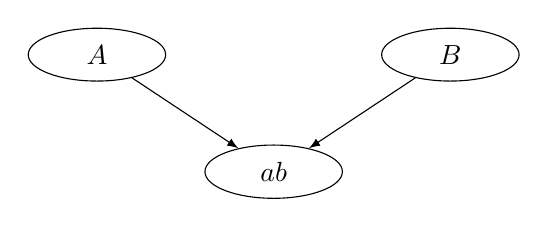
\begin{tikzpicture}[
  node distance=1cm and 1cm,
  mynode/.style={draw,ellipse,text width=1cm,align=center}
]
\node[mynode] (h1) {$A$};
\node[mynode, below right=of h1] (e) {$ab$};
\node[mynode, above right=of e] (h2) {$B$};
\path 
(h1) edge[-latex] (e)
(h2) edge[-latex] (e);
\end{tikzpicture}

\caption{Bayesian network with $ab$ resulting from $A$ and $B$.}
\label{network-ab}
\end{figure}
\end{center}

\hypertarget{but-sensitivity-depends-on-prior-probabilities}{%
\subsection{But Sensitivity Depends On Prior
Probabilities}\label{but-sensitivity-depends-on-prior-probabilities}}

We have shown, given a suitable number of assumptions, that the
sensitivity of \(a\wedge b\) can be greater relative to \(A \wedge B\)
than \(A\) alone. This explains why the evidential support of
\(a\wedge b\) is greater in favor of \(A \wedge B\) than alone \(A\).
Therefore---one might conclude---even factoring out differences in
priors probabiliies could still lead to differences in evidential
strength simply due to difference in sensitivity. But note that this
argument assumes that sensitivity---or specificity---have nothing to do
with prior probabilities.

Things are somewhat more complicated. After all,
\(\frac{\pr{a\wedge b \vert A}}{\pr{a\wedge b \vert A \wedge B}}=\frac{\pr{b \vert A}}{\pr{b \vert B}}\).
The denominator, which tracks the sensitivity of \(a\wedge b\) relative
to \(A\wedge B\) does not depend on the priors of \(A\wedge B\), but
solely on the sensitivty of \(a\) and \(b\) relative to \(A\) and \(B\).
However, the numerator, which tracks the sensitivity of \(a\wedge b\)
relative to \(a\), does depend on the priors of \(A\) (or whatvere other
hypothesis one choses to computer \(\pr{b \vert A}\) or \(\pr{b}\)).
This means that the denominator can vary depeding on the prior
probability of a chosen hypothesis. Thus, the lower the prior of \(A\),
the lower the probability of \(b\). One could still insist that here we
are not comparing the prior of a hypothesis, say \(B\), and the prior of
another hypothesis, say \(A \wedge B\). Whatever the difference in
sensitivity, it cannot be due to the difference in prior probabilities
of the hypotheses.\\
On other hand hand,
\(\frac{\pr{a\wedge b \vert A}}{\pr{a\wedge b \vert A \wedge B}}\) is
comparing two quantitities, one dependent on the priors and the other
not dependent on the priors.

More generally, the intuition that characteristics of the evidence such
as sensitivity and specificity should be indepedent of the probability
of the hypothesis of iterest turns out to be incorrect empirically. One
study in the medical literature has shown, surprisingly, that the
sensitivity of a diagnostic test is independent of the prior of the
hypothesis beign tested---say whether the patient has a medical
condition. However, specificity is dependent on the prior of the
hypothesis:

\begin{quote}
Overall, specificity tended to be
lower with higher disease prevalence; there
was no such systematic effect for sensitivity (page E537).
Source: Variation of a test’s sensitivity and specificity with disease prevalence Mariska M.G. Leeflang, Anne W.S. Rutjes, Johannes B. Reitsma, Lotty Hooft and Patrick M.M. Bossuyt
CMAJ August 06, 2013 185 (11) E537-E544; DOI: https://doi.org/10.1503/cmaj.121286
\end{quote}

\noindent The authors of the study, however, caution that

\begin{quote}
 Because sensitivity is estimated in
people with the disease of interest and specificity
in people without the disease of interest, changing the relative number of people 
with and without the disease of interest should not introduce
systematic differences. Therefore, the effects that
we found may be generated by other mechanisms that affect 
both prevalence and accuracy.
\end{quote}

So, according to the authors, changes in prevalence need not directly
affect specificity since variations in prevalence and variation in
specificity may have a common cause. Our earlier calculations about
combined specificity and sensitivity agree with experimental results,
namely, only specificity depends on the priors. Our calculations, in
fact, show that different priors for the individual claim do affect
specificity. The variation of specificity in the result of of splitting
the negation of the composite hypthesis \(\neg (A \wedge B)\) into three
further scenarios, \(\neg A \wedge B\), \(B \wedge \neg A\) and
\(\neg A \wedge neg B\). This prior sensitivity, of course, only applies
to composite hyotheses, but to some extent, any hypothesis can be
analyzed as a composite hypothesis. The claim that the defedant was
running down 5th avnue can be broken down in the conjuction that the
defendant was running and that the defendant was at 5th avenue. Any
claim, under some level of description, is a composite hypothesis. So,
perhpas, the quality or strength of the evidence should depend on the
the priors whether the hypothesis is composite or not. Is this another
example of base rate neglect?
\todo{M: Might be good to have a simulation here that makes vidid why combined specificity is in fact dependent on the priors. Maybe it is, after all, a fallacy 
to think that the quality/strength of the evidence should be independent of the priors. HELP!}

Let's grant that the quality of the evidence should depend, contrary to
our initial intuition, on the prior probability of the hypotheses. If
that is so, it would not be natural to see that evidence -- the same
evidence -- strongly favors \(A\wedge B\) without strongly favoring
\(A\) or \(B\). Perhaps we can make sense of this if we keep in mind the
comparison between hypothesis we are making here.

NOT SURE HOW TO CONTINUE HERE THOUGH!

TO DO:

\begin{enumerate}
\def\labelenumi{\arabic{enumi}.}
\item
  NOTE THAT EVEN BY EQUALIZING PRIORS, TE DISTRBUTION PARADOX DOES NOT
  GO AWAY. SO WHAT ELSE IS GOING ON HERE? NEED TO MAKE COMPATISON
  BETWEEN HYPOTHESES. NEED TO FIGURE THIS OUT!
\item
  TRY TO MAKE SENSE OF THIS, IT IS INTITVELY ACCEPTABLE THAT SUPPORT FOR
  COMBINED CLAIM, EVEN HOLDING FIXED THE SAME EVIDENCE, SHOULD BE
  STRONGER THEN SUPPORT FOR INDIVIDUAL CLAIM? THAT IS CLEARLY ODD AND
  GOES AGAINST COMMON ASSUMPTIONS.
\item
  \textbf{HYPOTHESIS: WHEN THE HYPTHESIS IS NOT MEDIATED (AS IN a toward A OR b TOWARD B, AS OPPOSED TO a TOWARD A-AND-B), THEN SENSITIVITY OR SPECICITIY IS NOT DEPEDENT ON PRIORS}
\end{enumerate}

\hypertarget{which-measure-of-combined-evidential-support}{%
\subsection{Which Measure of (Combined) Evidential
Support?}\label{which-measure-of-combined-evidential-support}}

THIGNS TO ADD:

\begin{enumerate}
\def\labelenumi{\arabic{enumi}.}
\item
  THE MIN SEEMS TO BE THE MEASURE FOR COMPOSITE CLAIMS THAT CAPTURES
  AGGREGATION AND DISTRIBUTION BEST. SO THE QUESTION IS WHAT
  PROBABILISTIC MEASURE CAPTURES MIN?
\item
  IS DEPEDENCY ON PRIOR ANOTHER EXAMPLE OF BASE RATE NEGLECT? WE NEGLECT
  BAE RATE IN CALCULATING POSTERIOR BUT ALSO IN CALCULATING STRENGTH OF
  EVIDENCE? WE JUST NEED TO LIVE WITH THE FACT THAT WE HAVE A POOR
  UNDERSTANDING OF EVIDENCE BUT PERHPAS GOOD ENOUGH TO GET BY IN THE
  WORLD. CONNECT TO POINT 1 AND MIN FUNCTION.
\end{enumerate}

\hypertarget{the-likelihood-strategy}{%
\subsection{The likelihood strategy}\label{the-likelihood-strategy}}

Focusing on posterior probabilities is not the only approach that legal
probabilists can pursue. By Bayes' theorem, the following holds, using
\(G\) and \(I\) as competing hypotheses:

\[ \frac{\Pr(G \vert E)}{\Pr(I \vert E)} = \frac{\Pr(E \vert G)}{\Pr(E \vert I)} \times \frac{\Pr(G)}{\Pr(I)},\]

or using \(H_p\) and \(H_d\) as competing hypotheses,

\[ \frac{\Pr(H_p \vert E)}{\Pr(H_d \vert E)} = \frac{\Pr(E \vert H_p)}{\Pr(E \vert H_d)} \times \frac{\Pr(H_p)}{\Pr(H_d)},\]

or in words

\[ \textit{posterior odds} = \textit{likelihood ratio} \times \textit{prior odds}.\]

A difficult problem is to assign numbers to the prior probabiliteis such
as \(\Pr(G)\) or \(\Pr(H_p)\), or priors odds such as
\(\frac{\Pr(G)}{\Pr(I)}\) or \(\frac{\Pr(H_p)}{\Pr(H_d)}\).

DISCUSS DIFFICULTIES ABOUT ASSIGNING PRIORS! WHERE? CAN WE USE IMPRECISE
PROBABILKITIES T TALK ABOUT PRIORS -- I.E. LOW PRIORS = TOTAL IGNORANCE
= VERY IMPRECISE (LARGE INTERVAL) PRIORS? THE PROBLME WITH THIS WOULD BE
THAT THERE IS NO UPDSATING POSSIBLE. ALL UPDATING WOULD STILL GET BACK
TO THE STARTING POINT. DO YOU HAVE AN ANSWER TO THAT? WOULD BE
INTERETSING TO DISCUSS THIS!

Given these difficulties, both practical and theoretical, one option is
to dispense with priors altogether. This is not implausible. Legal
disputes in both criminal and civil trials should be decided on the
basis of the evidence presented by the litigants. But it is the
likelihood ratio -- not the prior ratio -- that offers the best measure
of the overall strength of the evidece presented. So it is all too
natural to focus on likekihood ratios and leave the priors out of the
picture. If this is the right, the question is, how would a
probabilistic interpretation of standards of proof based on the
likelihood rato look like? At its simplest, this stratgey will look as
follows. Recall our discussion of expected utility theory:

\[ \text{convict provided}           \frac{cost(CI)}{cost(AG)} < \frac{\Pr(H_p \vert E)}{\Pr(H_d \vert E )}, \]

which is equivalent to

\[ \text{convict provided}           \frac{cost(CI)}{cost(AG)} < \frac{\Pr(E \vert H_p)}{\Pr(E \vert H_d)} \times \frac{\Pr(H_p)}{\Pr(H_d)}.\]

By rearraing the terms,

\[ \text{convict provided}  \frac{\Pr(E \vert H_p)}{\Pr(E \vert H_d)} > \frac{\Pr(H_d)}{\Pr(H_p)} \times     \frac{cost(CI)}{cost(AG)} .\]

Then, on this intepretation, the likelihood ratio should be above a
suitable threshold that is a function of the cost ratio and the prior
ratio. The outstanding question is how this threshold is to be
determined.

\hypertarget{kaplow}{%
\subsubsection{Kaplow}\label{kaplow}}

Quite independently, a similar approach to juridical decisions has been
proposed by Kaplow (2014) -- we'll call it
\textbf{decision-theoretic legal probabilism (DTLP)}. It turns out that
Cheng's suggestion is a particular case of this more general approach.
Let \(LR(E)=\pr{E\vert H_\Pi}/\pr{E\vert H_\Delta}\). In whole
generality, DTLP invites us to convict just in case \(LR(E)>LR^\star\),
where \(LR^\star\) is some critical value of the likelihood ratio.

Say we want to formulate the usual preponderance rule: convict iff
\(\pr{H_\Pi\vert E}>0.5\), that is, iff
\(\frac{\pr{H_\Pi\vert E}}{\pr{H_\Delta\vert E}}>1\). By Bayes' Theorem
we have:

\vspace{-6mm}

\begin{align*}
\frac{\pr{H_\Pi\vert E}}{\pr{H_\Delta\vert E}} =  \frac{\pr{H_\Pi}}{\pr{H_\Delta}}\times \frac{\pr{E\vert H_\Pi}}{\pr{E\vert H_\Delta}} &>1 \Leftrightarrow\\
  \Leftrightarrow \frac{\pr{E\vert H_\Pi}}{\pr{E\vert H_\Delta}} &> \frac{\pr{H_\Delta}}{\pr{H_\Pi}} 
 \end{align*} \noindent So, as expected, \(LR^\star\) is not unique and
depends on priors. Analogous reformulations are available for thresholds
other than \(0.5\).

Kaplow's point is not that we can reformulate threshold decision rules
in terms of priors-sensitive likelihood ratio thresholds. Rather, he
insists, when we make a decision, we should factor in its consequences.
Let \(G\) represent potential gain from correct conviction, and \(L\)
stand for the potential loss resulting from mistaken conviction. Taking
them into account, Kaplow suggests, we should convict if and only if:

\vspace{-6mm}

\begin{align}
\label{eq:Kaplow_decision}
\pr{H_\Pi\vert E}\times G > \pr{H_\Delta\vert E}\times L
\end{align} \noindent Now, \eqref{eq:Kaplow_decision} is equivalent to:

\vspace{-6mm}

\begin{align}
\nonumber
\frac{\pr{H_\Pi \vert E}}{\pr{H_\Delta \vert E}} & > \frac{L}{G}\\
\nonumber
\frac{\pr{H_\Pi}}{\pr{H_\Delta}} \times \frac{\pr{E\vert H_\Pi}}{\pr{E\vert H_\Delta}} &> \frac{L}{G}\\
\nonumber
\frac{\pr{E\vert H_\Pi}}{\pr{E\vert H_\Delta}}  & > \frac{\pr{H_\Delta}}{\pr{H_\Pi}} \times \frac{L}{G}\\
\label{eq:Kaplow_decision2} LR(E)  & > \frac{\pr{H_\Delta}}{\pr{H_\Pi}} \times \frac{L}{G}
\end{align}

\noindent This is the general format of Kaplow's decision standard.

\hypertarget{dawid}{%
\subsubsection{Dawid}\label{dawid}}

Here is a slightly different perspective, due to Dawid (1987), that also
suggests that juridical decisions should be likelihood-based. The focus
is on witnesses for the sake of simplicity. Imagine the plaintiff
produces two independent witnesses: \(W_A\) attesting to \(A\), and
\(W_B\) attesting to \(B\). Say the witnesses are regarded as \(70\%\)
reliable and \(A\) and \(B\) are probabilistically independent, so we
infer \(\pr{A}=\pr{B}=0.7\) and \(\pr{A\et B}=0.7^2=0.49\).

But, Dawid argues, this is misleading, because to reach this result we
misrepresented the reliability of the witnesses: \(70\%\) reliability of
a witness, he continues, does not mean that if the witness testifies
that \(A\), we should believe that \(\pr{A}=0.7\). To see his point,
consider two potential testimonies:

\begin{center}
\begin{tabular}
{@{}ll@{}}
\toprule
  $A_1$ & The sun rose today. \\
   $A_2$ & The sun moved backwards through the sky today.\\
\bottomrule
\end{tabular}
\end{center}

\noindent     Intuitively, after hearing them, we would still take
\(\pr{A_1}\) to be close to 1 and \(\pr{A_2}\) to be close to 0, because
we already have fairly strong convictions about the issues at hand. In
general, how we should revise our beliefs in light of a testimony
depends not only on the reliability of the witness, but also on our
prior
convictions.\footnote{An issue that Dawid does not bring up is the interplay between our priors and our assessment of the reliability of the witnesses. Clearly, our posterior assessment of the credibility of the witness who testified $A_2$ will be lower than that of the other witness.}
And this is as it should be: as indicated by Bayes' Theorem, one and the
same testimony with different priors might lead to different posterior
probabilities.

So far so good. But how should we represent evidence (or testimony)
strength then? Well, one pretty standard way to go is to focus on how
much it contributes to the change in our beliefs in a way independent of
any particular choice of prior beliefs. Let \(a\) be the event that the
witness testified that \(A\). It is useful to think about the problem in
terms of \emph{odds, conditional odds (O)} and
\emph{likelihood ratios (LR)}:
\begin{align*} O(A)  & = \frac{\pr{A}}{\pr{\n A}}\\
 O(A\vert a) &= \frac{\pr{A\vert a}}{\pr{\n A \vert a}}  \\
 LR(a\vert A) &= \frac{\pr{a\vert A}}{\pr{a\vert \n A}}. 
\end{align*}

Suppose our prior beliefs and background knowledge, before hearing a
testimony, are captured by the prior probability measure
\(\prr{\cdot}\), and the only thing that we learn is \(a\). We're
interested in what our \emph{posterior} probability measure,
\(\prp{\cdot}\), and posterior odds should then be. If we're to proceed
with Bayesian updating, we should have:

\vspace{-6mm}

\begin{align*}
 \frac{\prp{A}}{\prp{\n A}} & = \frac{\prr{A\vert a}}{\prr{\n A\vert a}}
 =
 \frac{\prr{a\vert A}}{\prr{a\vert \n A}}
 \times
 \frac{\prr{A}}{\prr{\n A}}
  \end{align*} that is,

\vspace{-6mm}

\begin{align}
 \label{bayesodss2}
 O_{posterior}(A)& = O_{prior}(A\vert a) = \!\!\!\!\!  \!\!\!\!\!  \!\! \!\!  \underbrace{LR_{prior}(a\vert A)}_{\mbox{\footnotesize conditional likelihood ratio}}  \!\!\!\!\!   \!\!\!\!\!  \!\! \!\!   \times  O_{prior}(A)
 \end{align}

The conditional likelihood ratio seems to be a much more direct measure
of the value of \(a\), independent of our priors regarding \(A\) itself.
In general, the posterior probability of an event will equal to the
witness's reliability in the sense introduced above only if the prior is
\(1/2\).\footnote{Dawid gives no general argument, but it is not too hard to  give one. Let $rel(a)=\pr{a\vert A}=\pr{\n a\vert \n A}$. We have in the background $\pr{a\vert \n A}=1-\pr{\n a\vert \n A}=1-rel(a)$.
 We want to find the condition under which $\pr{A\vert a} = \pr{a\vert A}$. Set $\pr{A}=p$ and  start with Bayes' Theorem and the law of total probability, and go from there:
 \begin{align*}
 \pr{A\vert a}& = \pr{a\vert A}\\
 \frac{\pr{a\vert A}p}{\pr{a\vert A}p+\pr{a\vert \n A}(1-p)} &= \pr{a\vert A} \\
 \pr{a\vert A}p & = \pr{a\vert A}[\pr{a\vert A}p+\pr{a\vert \n A}(1-p)]\\
 p & = \pr{a\vert A}p + \pr{a\vert \n A} - \pr{a\vert \n A}p\\
 p &= rel(a) p + 1-rel(a)- (1-rel(a))p\\
 p & = rel(a)p +1 - rel(a) -p +rel(a)p \\
 2p & =  2rel(a)p + 1 - rel(a)  \\
 2p - 2 rel(a)p & = 1-rel(a)\\
 2p(1-rel(a)) &= 1-rel(a)\\
 2p & = 1
 \end{align*}

\noindent  First we multiplied both sides by the denominator. Then we divided both sides by $\pr{a\vert A}$ and multiplied on the right side. Then we used our background notation and information. Next, we manipulated the right-hand side algebraically and  moved  $-p$ to the left-hand side. Move $2rel(a)p$ to the left and manipulate the result algebraically to get to the last line.}

\hypertarget{likelihood-and-dac}{%
\subsection{Likelihood and DAC}\label{likelihood-and-dac}}

But how does our preference for the likelihood ratio as a measure of
evidence strength relate to DAC? Let's go through Dawid's reasoning.

A sensible way to probabilistically interpret the \(70\%\) reliability
of a witness who testifies that \(A\) is to take it to consist in the
fact that the probability of a positive testimony if \(A\) is the case,
just as the probability of a negative testimony (that is, testimony that
\(A\) is false) if \(A\) isn't the case, is
0.7:\footnote{In general setting, these are called the \emph{sensitivity} and \emph{specificity} of a test (respectively), and they don't have to be equal. For instance, a degenerate test for an illness which always responds positively, diagnoses everyone as ill, and so has sensitivity 1, but specificity 0.}
\[\prr{a\vert A}=\prr{\n a\vert\n  A}=0.7.\]
\noindent   \(\prr{a\vert \n A}=1- \prr{\n a\vert \n A}=0.3\), and so
the same information is encoded in the appropriate likelihood ratio:
\[LR_{prior}(a\vert A )=\frac{\prr{a\vert A}}{\prr{a\vert \n A}}= \frac{0.7}{0.3}\]

Let's say that \(a\) \emph{provides (positive) support} for \(A\) in
case \[O_{posterior}(A)=O_{prior}(A\vert a)> O_{prior}(A)\]
\noindent  that is, a testimony \(a\) supports \(A\) just in case the
posterior odds of \(A\) given \(a\) are greater than the prior odds of
\(A\) (this happens just in case \(\prp{A}>\prr{A}\)). By
\eqref{bayesodss2}, this will be the case if and only if
\(LR_{prior}(a\vert A)>1\).

One question that Dawid addresses is this: assuming reliability of
witnesses \(0.7\), and assuming that \(a\) and \(b\), taken separately,
provide positive support for their respective claims, does it follow
that \(a \et b\) provides positive support for \(A\et B\)?

Assuming the independence of the witnesses, this will hold in
non-degenerate cases that do not involve extreme probabilities, on the
assumption of independence of \(a\) and \(b\) conditional on all
combinations: \(A\et B\), \(A\et \n B\), \(\n A \et B\) and
\(\n A \et \n B\).\footnote{Dawid only talks about the independence of witnesses without reference to  conditional independence. Conditional independence does not follow from independence, and it is the former that is needed here (also, four non-equivalent different versions of it).}\(^,\)\textasciitilde{}\footnote{In terms of notation and derivation in the optional content that will follow, the claim holds  if and only if $28 > 28 p_{11}-12p_{00}$.  This inequality is not  true for all admissible values of $p_{11}$ and $p_{00}$. If $p_{11}=1$ and $p_{00}=0$, the sides are equal. However, this is a rather degenerate example. Normally, we are  interested in cases where $p_{11}< 1$. And indeed, on this assumption, the inequality holds.}

Let us see why the above claim holds. The calculations are my
reconstruction and are not due to Dawid. The reader might be annoyed
with me working out the mundane details of Dawid's claims, but it turns
out that in the case of Dawid's strategy, the devil is in the details.
The independence of witnesses gives us: \begin{align*}
 \pr{a \et b \vert A\et B}& =0.7^2=0.49\\
 \pr{a \et b \vert A\et \n B}& =  0.7\times 0.3=0.21\\
 \pr{a \et b \vert \n A\et B}& =  0.3\times 0.7=0.21\\
 \pr{a \et b \vert \n A\et \n B}& =  0.3\times 0.3=0.09
 \end{align*} Without assuming \(A\) and \(B\) to be independent, let
the probabilities of \(A\et B\), \(\n A\et B\), \(A\et \n B\),
\(\n A\et \n B\) be \(p_{11}, p_{01}, p_{10}, p_{00}\). First, let's see
what \(\pr{a\et b}\) boils down to.

By the law of total probability we have:
\begin{align}\label{eq:total_lower}
 \pr{a\et b} & = 
                     \pr{a\et b \vert A \et B}\pr{A\et B} + \\ &  \nonumber
                     +\pr{a\et b \vert A \et \n B}\pr{A\et \n B} \\ &  \nonumber
 + \pr{a\et b \vert \n A \et B}\pr{\n A\et B} + \\ & \nonumber
                     + \pr{a\et b \vert \n A \et \n B}\pr{\n A\et \n B}
 \end{align} \noindent which, when we substitute our values and
constants, results in: \begin{align*}
                     & = 0.49p_{11}+0.21(p_{10}+p_{01})+0.09p_{00}
 \end{align*} Now, note that because \(p_{ii}\)s add up to one, we have
\(p_{10}+p_{01}=1-p_{00}-p_{11}\). Let us continue. \begin{align*}
    & = 0.49p_{11}+0.21(1-p_{00}-p_{11})+0.09p_{00} \\
                     & = 0.21+0.28p_{11}-0.12p_{00}
 \end{align*}

Next, we ask what the posterior of \(A\et B\) given \(a\et b\) is (in
the last line, we also multiply the numerator and the denominator by
100). \begin{align*}
 \pr{A\et B\vert a \et b} & =
         \frac{\pr{a\et b \vert A \et B}\pr{A\et B}}
             {\pr{a\et b}}\\
         & =
                     \frac{49p_{11}}
                           {21+28p_{11}-12p_{00}} 
         \end{align*}

In this particular case, then, our question whether
\(\pr{A\et B\vert a\et b}>\pr{A\et B}\) boils down to asking whether
\[\frac{49p_{11}}{21+28p_{11}-12p_{00}}> p_{11}\] that is, whether
\(28 > 28 p_{11}-12p_{00}\) (just divide both sides by \(p_{11}\),
multiply by the denominator, and manipulate algebraically).

Dawid continues working with particular choices of values and provides
neither a general statement of the fact that the above considerations
instantiate nor a proof of it. In the middle of the paper he says:

\begin{quote}
 Even under prior dependence, the combined support is always positive, in the sense that the posterior probability of the case always exceeds its prior probability\dots When the problem is analysed carefully, the `paradox' evaporates [pp. 95-7]\end{quote}

\noindent where he still means the case with the particular values that
he has given, but he seems to suggest that the claim generalizes to a
large array of cases.

The paper does not contain a precise statement making the conditions
required explicit and, \emph{a fortriori}, does not contain a proof of
it. Given the example above and Dawid's informal reading, let us develop
a more precise statement of the claim and a proof thereof.

\begin{fact}\label{ther:increase}
Suppose that  $rel(a),rel(b)>0.5$ and witnesses are independent conditional on all Boolean combinations of $A$ and $B$  (in a sense to be specified), and that none of the Boolean combinations of $A$ and $B$ has an extreme probability (of 0 or 1). It follows that  $\pr{A\et B \vert a\et b}>\pr{A\et B}$. (Independence of $A$ and $B$ is not required.)
\end{fact}

Roughly, the theorem says that if independent and reliable witnesses
provide positive support of their separate claims, their joint testimony
provides positive support of the conjunction of their claims.

Let us see why the claim holds. First, we introduce an abbreviation for
witness reliability:
\begin{align*}\mathbf{a} &=rel(a)=\pr{a\vert A}=\pr{\n a\vert \n A}>0.5\\ 
\mathbf{b} &=rel(b)=\pr{b\vert B}=\pr{\n b\vert \n A}>0.5
\end{align*} Our independence assumption means: \begin{align*}
\pr{a\et b \vert A\et B}  &= \mathbf{ab}\\
\pr{a\et b \vert A\et \n B} & = \mathbf{a(1-b)}\\
\pr{a\et b \vert \n A\et B}  & = \mathbf{(1-a)b}\\
\pr{a\et b \vert \n A\et \n  B}  & = \mathbf{(1-a)(1-b)}
\end{align*}

\vspace{-2mm}

Abbreviate the probabilities the way we already did:

\begin{center}
\begin{tabular}{ll}
$\pr{A\et B} = p_{11}$ & $\pr{A\et \n B} = p_{10}$\\
$\pr{\n A \et B} = p_{01}$ & $\pr{\n A \et \n B}=p_{00}$
\end{tabular}
\end{center}

Our assumptions entail \(0\neq p_{ij}\neq 1\) for \(i,j\in \{0,1\}\)
and: \begin{align}\label{eq:sumupto1}
p_{11}+p_{10}+p_{01}+p_{00}&=1
\end{align}

\noindent So, we can use this with \eqref{eq:total_lower} to get:
\begin{align}\label{eq:aetb}
\pr{a\et b} & =  \mathbf{ab}p_{11} + \mathbf{a(1-b)}p_{10}+\mathbf{(1-a)b}p_{01} + \mathbf{(1-a)(1-b)}p_{00}\\ \nonumber
& = p_{11}\mathbf{ab} + p_{10}(\mathbf{a}-\mathbf{ab}) + p_{01}(\mathbf{b}-\mathbf{ab})+p_{00}(1-\mathbf{b}-\mathbf{a}+\mathbf{ab})
\end{align}

Let's now work out what the posterior of \(A\et B\) will be, starting
with an application of the Bayes' Theorem: \begin{align} \nonumber
\pr{A\et B \vert a\et b} & = \frac{\pr{a\et b \vert A \et B}\pr{A\et B}}{\pr{a\et b}}
\\ \label{eq:boiled}
& = \frac{\mathbf{ab}p_{11}}{p_{11}\mathbf{ab} + p_{10}(\mathbf{a}-\mathbf{ab}) + p_{01}(\mathbf{b}-\mathbf{ab})+p_{00}(1-\mathbf{b}-\mathbf{a}+\mathbf{ab})}
\end{align} To answer our question we therefore have to compare the
content of \eqref{eq:boiled} to \(p_{11}\) and our claim holds just in
case: \begin{align*}
\frac{\mathbf{ab}p_{11}}{p_{11}\mathbf{ab} + p_{10}(\mathbf{a}-\mathbf{ab}) + p_{01}(\mathbf{b}-\mathbf{ab})+p_{00}(1-\mathbf{b}-\mathbf{a}+\mathbf{ab})} &> p_{11}
\end{align*} \begin{align*}
 \frac{\mathbf{ab}}{p_{11}\mathbf{ab} + p_{10}(\mathbf{a}-\mathbf{ab}) + p_{01}(\mathbf{b}-\mathbf{ab})+p_{00}(1-\mathbf{b}-\mathbf{a}+\mathbf{ab})} & > 1\end{align*}
\begin{align}  
 \label{eq:goal}
p_{11}\mathbf{ab} + p_{10}(\mathbf{a}-\mathbf{ab}) + p_{01}(\mathbf{b}-\mathbf{ab})+p_{00}(1-\mathbf{b}-\mathbf{a}+\mathbf{ab}) & < \mathbf{ab}
\end{align} Proving \eqref{eq:goal} is therefore our goal for now. This
is achieved by the following
reasoning:\footnote{Thanks to Pawel Pawlowski for working on this proof with me.}

\hspace{-7mm}
\resizebox{13.5cm}{!}{
\begin{tabular}{llr}
 1. & $\mathbf{b}>0.5,\,\,\, \mathbf{a}>0.5$ & \mbox{assumption}\\
 2. & $2\mathbf{b}>1,\,\,\, 2\mathbf{a}> 1$ & \mbox{from 1.}\\
 3. & $2\mathbf{ab}>\mathbf{a},\,\,\, 2\mathbf{ab}>\mathbf{b}$ & \mbox{multiplying by $\mathbf{a}$ and $\mathbf{b}$ respectively}\\
 4.  & $p_{10}2\mathbf{ab}>p_{10}\mathbf{a}$,\,\,\, $p_{01}2\mathbf{ab}>p_{01}\mathbf{b}$ & \mbox{multiplying by $p_{10}$ and $p_{01}$ respectively}\\
 5.  & $p_{10}2\mathbf{ab} +  p_{01}2\mathbf{ab} > p_{10}\mathbf{a} + p_{01}\mathbf{b}$ & \mbox{adding by sides, 3., 4.}\\
 6. & $1- \mathbf{b}- \mathbf{a} <0$ & \mbox{from 1.}\\
 7. & $p_{00}(1-\mathbf{b}-\mathbf{a})<0$ & \mbox{From 6., because $p_{00}>0$}\\
  8.  &  $p_{10}2\mathbf{ab} +  p_{01}2\mathbf{ab} > p_{10}\mathbf{a} + p_{01}\mathbf{b} + p_{00}(1-\mathbf{b}-\mathbf{a})$ & \mbox{from 5. and 7.}\\
  9.  & $p_{10}\mathbf{ab} + p_{10}\mathbf{ab} + p_{01}\mathbf{ab} + p_{01}\mathbf{ab} + p_{00}\mathbf{ab} - p_{00}\mathbf{ab}> p_{10}\mathbf{a} + p_{01}\mathbf{b} + p_{00}(1-\mathbf{b}-\mathbf{a})$ & \mbox{8., rewriting left-hand side}\\
  10.  & $p_{10}\mathbf{ab} + p_{01}\mathbf{ab}  + p_{00}\mathbf{ab} > - p_{10}\mathbf{ab}  -  p_{01}\mathbf{ab} + p_{00}\mathbf{ab} +  p_{10}\mathbf{a} + p_{01}\mathbf{b} + p_{00}(1-\mathbf{b}-\mathbf{a})$ &  \mbox{9., moving from left to right}\\
11. & $\mathbf{ab}(p_{10}+p_{01}+p_{00})> p_{10}(\mathbf{a}-\mathbf{ab})+p_{01}(\mathbf{b}-\mathbf{ab})+p_{00}(1-\mathbf{b}-\mathbf{a}+\mathbf{ab})$ & \mbox{10., algebraic manipulation}\\
12. & $\mathbf{ab}(1-p_{11})> p_{10}(\mathbf{a}-\mathbf{ab})+p_{01}(\mathbf{b}-\mathbf{ab})+p_{00}(1-\mathbf{b}-\mathbf{a}+\mathbf{ab})$ & \mbox{11. and equation \eqref{eq:sumupto1}}\\
13. & $\mathbf{ab}- \mathbf{ab}p_{11}> p_{10}(\mathbf{a}-\mathbf{ab})+p_{01}(\mathbf{b}-\mathbf{ab})+p_{00}(1-\mathbf{b}-\mathbf{a}+\mathbf{ab})$ & \mbox{12., algebraic manipulation}\\
14. & $\mathbf{ab}> \mathbf{ab}p_{11}+ p_{10}(\mathbf{a}-\mathbf{ab})+p_{01}(\mathbf{b}-\mathbf{ab})+p_{00}(1-\mathbf{b}-\mathbf{a}+\mathbf{ab})$ & \mbox{13., moving from left to right}\\
\end{tabular}}

\%\textbackslash end\{adjustbox\}

\vspace{1mm}

The last line is what we have been after.

\intermezzob

Now that we have as a theorem an explication of what Dawid informally
suggested, let's see whether it helps the probabilist handling of DAC.

\hypertarget{kaplow-1}{%
\subsubsection{Kaplow}\label{kaplow-1}}

On RLP, at least in certain cases, the decision rule leads us to
\eqref{eq:Cheng:compar2}, which tells us to decide the case based on
whether the likelihood ratio is greater than 1.

\footnote{Again, the name of the view is by no means standard, it is  just a term I coined to refer to various types of legal probabilism in a fairly uniform manner.}
While Kaplow did not discuss DAC or the gatecrasher paradox, it is only
fair to evaluate Kaplow's proposal from the perspective of these
difficulties.

Add here stuff from Marcello's Mind paper about the prisoner
hypothetical. Then, discuss Rafal's critique of the likelihood ratio
threshold and see where we end up.

\hypertarget{dawids-likelihood-strategy-doesnt-help}{%
\subsection{Dawid's likelihood strategy doesn't
help}\label{dawids-likelihood-strategy-doesnt-help}}

Recall that DAC was a problem posed for the decision standard proposed
by TLP, and the real question is how the information resulting from Fact
\ref{ther:increase} can help to avoid that problem. Dawid does not
mention any decision standard, and so addresses quite a different
question, and so it is not clear that `\texttt{the}paradox'
evaporates'\,', as Dawid suggests.

What Dawid correctly suggests (and we establish in general as Fact
\ref{ther:increase}) is that the support of the conjunction by two
witnesses will be positive as soon as their separate support for the
conjuncts is positive. That is, that the posterior of the conjunction
will be higher that its prior. But the critic of probabilism never
denied that the conjunction of testimonies might raise the probability
of the conjunction if the testimonies taken separately support the
conjuncts taken separately. Such a critic can still insist that Fact
\ref{ther:increase} does nothing to alleviate her concern. After all, at
least \emph{prima facie} it still might be the case that:

\begin{itemize}
\item  the posterior probabilities of the conjuncts are above a given threshold,
\item   the posterior probability of the conjunction is higher than the prior probability of the conjunction,
\item   the posterior probability of the conjunction 
 is still below the threshold.
\end{itemize}

That is, Fact \ref{ther:increase} does not entail that once the
conjuncts satisfy a decision standard, so does the conjunction.

At some point, Dawid makes a general claim that is somewhat stronger
than the one already cited:

\begin{quote} When the problem is analysed carefully, the `paradox' evaporates: suitably measured, the support supplied by the conjunction of several independent testimonies exceeds that supplied by any of its constituents.

  [p. 97]\end{quote}

This is quite a different claim from the content of Fact
\ref{ther:increase}, because previously the joint probability was
claimed only to increase as compared to the prior, and here it is
claimed to increase above the level of the separate increases provided
by separate testimonies. Regarding this issue Dawid elaborates (we still
use the \(p_{ij}\)-notation that we've already introduced):

\begin{quote}
 ``More generally, let $\pr{a\vert A}/\pr{a\vert \n A}=\lambda$, $\pr{b\vert B}/\pr{b\vert \n B}=\mu$, with $\lambda, \mu >0.7$, as might arise, for example, when there are several available testimonies. If the witnesses are
  independent, then \[\pr{A\et B\vert  a\et b} = \lambda \mu p_{11}/(\lambda \mu p_{11} + \lambda p_{10} +\mu p_{01} + p_{00})\] which  increases with
 each of $\lambda$ and $\mu$, and is never less than the larger of $\lambda p_{11}/(1-p_{11}+\lambda p_{11}),
 \mu p_{11} /(1- p_{11} 1 + \mu p_{11})$, the posterior probabilities appropriate to the individual testimonies.'' [p. 95]
 \end{quote}

This claim, however, is false.

\intermezzoa

Let us see why. The quoted passage is a bit dense. It contains four
claims for which no arguments are given in the paper. The first three
are listed below as \eqref{eq:lambdamu}, the fourth is that if the
conditions in \eqref{eq:lambdamu} hold,
\(\pr{A\et B\vert a\et b}>max(\pr{A\vert a},\pr{B\vert b})\). Notice
that \(\lambda=LR(a\vert A)\) and \(\mu=LR(b\vert B)\). Suppose the
first three claims hold, that is: \begin{align}\label{eq:lambdamu}
 \pr{A\et B\vert  a\et b} &= \lambda \mu p_{11}/(\lambda \mu p_{11} + \lambda p_{10} +\mu p_{01} + p_{00})\\
 \pr{A\vert a} & = \frac{\lambda p_{11}}{1-p_{11}+\lambda p_{11}}\nonumber \\
 \pr{B\vert b} & = \frac{\mu p_{11}}{1-p_{11}+\mu p_{11}} \nonumber 
 \end{align} \noindent Is it really the case that
\(\pr{A\et B\vert a\et b}>\pr{A\vert a},\pr{B\vert b}\)? It does not
seem so. Let \(\mathbf{a}=\mathbf{b}=0.6\),
\(pr =\la p_{11},p_{10},p_{01},p_{00}\ra=\la 0.1, 0.7, 0.1, 0.1 \ra\).
Then, \(\lambda=\mu=1.5>0.7\) so the assumption is satisfied. Then we
have \(\pr{A}=p_{11}+p_{10}=0.8\), \(\pr{B}=p_{11}+p_{01}=0.2\). We can
also easily compute
\(\pr{a}=\mathbf{a}\pr{A}+(1-\mathbf{a})\pr{\n A}=0.56\) and
\(\pr{b}=\mathbf{b}\pr{B}+(1-\mathbf{b})\pr{\n B}=0.44\). Yet:

\begin{align*}
 \pr{A\vert a} & = \frac{\pr{a\vert A}\pr{A}}{\pr{a}} = \frac{0.6\times 0.8}{0.6\times 0.8 + 0.4\times 0.2}\approx 0.8571 \\
 \pr{B\vert b} & = \frac{\pr{b\vert B}\pr{B}}{\pr{b}} = \frac{0.6\times 0.2}{0.6\times 0.2 + 0.4\times 0.8}\approx 0.272 \\
 \pr{A\et B \vert a \et b} & = \frac{\pr{a\et b\vert A \et B}\pr{A\et B}}{\splitfrac{\pr{a\et b \vert A\et B}\pr{A\et B}+
   \pr{a\et b\vert A\et \n B}\pr{A\et \n B} +}{+ 
 \pr{a\et b \vert \n A \et B}\pr{\n A \et B} + \pr{a\et b \vert \n A \et \n B}\pr{\n A \et \n B}}} \\
 & = \frac{\mathbf{ab}p_{11}}{
   \mathbf{ab}p_{11} + \mathbf{a}(1-\mathbf{b})p_{10} + (1-\mathbf{a})\mathbf{b}p_{01} + (1-\mathbf{a})(1-\mathbf{b})p_{00}
 }  
    \approx 0.147
 \end{align*} The posterior probability of \(A\et B\) is not only lower
than the larger of the individual posteriors, but also lower than any of
them!

So what went wrong in Dawid's calculations in \eqref{eq:lambdamu}? Well,
the first formula is correct. However, let us take a look at what the
second one says (the problem with the third one is pretty much the
same): \begin{align*}
\pr{A\vert a } & = \frac{\frac{\pr{a\vert A}}{\pr{\n a \vert A}}\times \pr{A\et B}}{\pr{\n (A\et B)}+ \frac{\pr{a\vert A}}{\pr{\n a \vert A}} \times \pr{A\et B}}
\end{align*} Quite surprisingly, in Dawid's formula for
\(\pr{A\vert a}\), the probability of \(A\et B\) plays a role. To see
that it should not take any \(B\) that excludes \(A\) and the formula
will lead to the conclusion that \emph{always} \(\pr{A\vert a}\) is
undefined. The problem with Dawid's formula is that instead of
\(p_{11}=\pr{A\et B}\) he should have used \(\pr{A}=p_{11}+p_{10}\), in
which case the formula would rather say this: \begin{align*}
\pr{A\vert a } & = \frac{\frac{\pr{a\vert A}}{\pr{\n a \vert A}}\times \pr{A}}{\pr{\n A}+ \frac{\pr{a\vert A}}{\pr{\n a \vert A}} \times \pr{A}}\\
& = \frac{\frac{\pr{a\vert A}\pr{A}}{\pr{\n a \vert A}}}{\frac{\pr{\n a\vert A}\pr{\n A}}{\pr{\n a\vert A}}+ \frac{\pr{a\vert A}\pr{A}}{\pr{\n a \vert A}}}\\
& = \frac{\pr{a\vert A}\pr{A}}{\pr{\n a\vert A}\pr{\n A} + \pr{a\vert A}\pr{A}}
\end{align*} Now, on the assumption that witness' sensitivity is equal
to their specificity, we have \(\pr{a\vert \n A}=\pr{\n a \vert A}\) and
can substitute this in the denominator:
\begin{align*} & = \frac{\pr{a\vert A}\pr{A}}{\pr{ a\vert \n A}\pr{\n A} + \pr{a\vert A}\pr{A}}\end{align*}
and this would be a formulation of Bayes' theorem. And indeed with
\(\pr{A}=p_{11}+p_{10}\) the formula works (albeit its adequacy rests on
the identity of \(\pr{a\vert \n A}\) and \(\pr{\n a \vert A}\)), and
yields the result that we already obtained: \begin{align*}
\pr{A\vert a} &= \frac{\lambda(p_{11}+p_{10})}{1-(p_{11}+p_{10})+\lambda(p_{11}+p_{10})}\\
&= \frac{1.5\times 0.8}{1- 0.8+1.5\times 0.8} \approx 0.8571
\end{align*}

The situation cannot be much improved by taking \(\mathbf{a}\) and
\(\mathbf{b}\) to be high. For instance, if they're both 0.9 and
\(pr=\la0.1, 0.7, 0.1, 0.1 \ra\), the posterior of \(A\) is
\(\approx 0.972\), the posterior of \(B\) is \(\approx 0.692\), and yet
the joint posterior of \(A\et B\) is \(0.525\).

The situation cannot also be improved by saying that at least if the
threshold is 0.5, then as soon as \(\mathbf{a}\) and \(\mathbf{b}\) are
above 0.7 (and, \emph{a fortriori}, so are \(\lambda\) and \(\mu\)), the
individual posteriors being above 0.5 entails the joint posterior being
above 0.5 as well. For instance, for \(\mathbf{a}=0.7\) and
\(\mathbf{b}=0.9\) with \(pr= \la 0.1, 0.3, 0.5, 0.1\ra\), the
individual posteriors of \(A\) and \(B\) are \(\approx 0.608\) and
\(\approx 0.931\) respectively, while the joint posterior of \(A\et B\)
is \(\approx 0.283\).

\intermezzob

The situation cannot be improved by saying that what was meant was
rather that the joint likelihood is going to be at least as high as the
maximum of the individual likelihoods, because quite the opposite is the
case: the joint likelihood is going to be lower than any of the
individual ones.

\intermezzoa

Let us make sure this is the case. We have: \begin{align*}
 LR(a\vert A) & = \frac{\pr{a\vert A}}{\pr{a\vert \n A}}\\
 &= \frac{\pr{a\vert A}}{\pr{\n a\vert  A}} \\
& =  \frac{\mathbf{a}}{\mathbf{1-a}}.
\end{align*} where the substitution in the denominator is legitimate
only because witness' sensitivity is identical to their specificity.

With the joint likelihood, the reasoning is just a bit more tricky. We
will need to know what \(\pr{a\et b \vert \n (A\et B)}\) is. There are
three disjoint possible conditions in which the condition holds:
\(A\et \n B, \n A \et B\), and \(\n A \et \n B\). The probabilities of
\(a\et b\) in these three scenarios are respectively
\(\mathbf{a(1-b),(1-a)b,(1-a)(1-b)}\) (again, the assumption of
independence is important), and so on the assumption \(\n(A\et B)\) the
probability of \(a\et b\) is: \begin{align*}
\pr{a\et b \vert \n (A\et B)} & = 
\mathbf{a}(1-\mathbf{b})+(1-\mathbf{a})\mathbf{b}+(1-\mathbf{a})(1-\mathbf{b})\\ 
& = 
\mathbf{a}(1-\mathbf{b})+(1-\mathbf{a})(\mathbf{b} + 1-\mathbf{b})\\
& = \mathbf{a}(1-\mathbf{b})+(1-\mathbf{a})\\
& = \mathbf{a}-\mathbf{a}\mathbf{b}+1-\mathbf{a} = 1- \mathbf{a}\mathbf{b}
\end{align*} So, on the assumption of witness independence, we have:
\begin{align*}
LR(a\et b \vert A \et B) & = \frac{\pr{a\et b \vert A \et B}}{\pr{a \et b\vert \n (A \et B)}} \\
& = \frac{\mathbf{ab}}{\mathbf{1-ab}}
\end{align*}

With \(0<\mathbf{a},\mathbf{b}<1\) we have \(\mathbf{ab}<\mathbf{a}\),
\(1-\mathbf{ab}>1-\mathbf{a}\), and consequently:
\[\frac{\mathbf{ab}}{\mathbf{1-ab}} < \frac{\mathbf{a}}{\mathbf{1-a}}\]
which means that the joint likelihood is going to be lower than any of
the individual ones.

\intermezzob

Fact \ref{ther:increase} is so far the most optimistic reading of the
claim that if witnesses are independent and fairly reliable, their
testimonies are going to provide positive support for the
conjunction,\textbackslash footnote\{And this is the reading that Dawid
in passing suggests: ``the combined support is always positive, in the
sense that the posterior probability of the case always exceeds its
prior probability.'\,' (Dawid, 1987: 95) and any stronger reading of
Dawid's suggestions fails. But Fact \ref{ther:increase} is not too
exciting when it comes to answering the original DAC. The original
question focused on the adjudication model according to which the
deciding agents are to evaluate the posterior probability of the whole
case conditional on all evidence, and to convict if it is above a
certain threshold. The problem, generally, is that it might be the case
that the pieces of evidence for particular elements of the claim can
have high likelihood and posterior probabilities of particular elements
can be above the threshold while the posterior joint probability will
still fail to meet the threshold. The fact that the joint posterior will
be higher than the joint prior does not help much. For instance, if
\(\mathbf{a}=\mathbf{b}=0.7\), \(pr=\la 0.1, 0.5, 0.3, 0.1\ra\), the
posterior of \(A\) is \(\approx 0.777\), the posterior of \(B\) is
\(\approx 0.608\) and the joint posterior is \(\approx 0.216\) (yes, it
is higher than the joint prior \(=0.1\), but this does not help the
conjunction to satisfy the decision standard).

To see the extent to which Dawid's strategy is helpful here, perhaps the
following analogy might be useful.\\
Imagine it is winter, the heating does not work in my office and I am
quite cold. I pick up the phone and call maintenance. A rather cheerful
fellow picks up the phone. I tell him what my problem is, and he reacts:

\vspace{1mm}

\begin{tabular}{lp{10cm}}
 --- & Oh, don't worry. \\
 --- & What do you mean? It's cold in here! \\
 --- & No no, everything is fine, don't worry.\\
 --- & It's not fine! I'm cold here! \\
 --- & Look, sir, my notion of it being warm in your office is that the building provides some improvement to what the situation would be if it wasn't there. And you agree that you're definitely warmer than you'd be if your desk was standing outside, don't you? Your, so to speak, posterior warmth is higher than your prior warmth, right? 
 \end{tabular}
 \vspace{1mm}

Dawid's discussion is in the vein of the above conversation. In response
to a problem with the adjudication model under consideration Dawid
simply invites us to abandon thinking in terms of it and to abandon
requirements crucial for the model. Instead, he puts forward a fairly
weak notion of support (analogous to a fairly weak sense of the building
providing improvement), according to which, assuming witnesses are
fairly reliable, if separate fairly reliable witnesses provide positive
support to the conjuncts, then their joint testimony provides positive
support for the conjunction.

As far as our assessment of the original adjudication model and dealing
with DAC, this leaves us hanging. Yes, if we abandon the model, DAC does
not worry us anymore. But should we? And if we do, what should we change
it to, if we do not want to be banished from the paradise of
probabilistic methods?

Having said this, let me emphasize that Dawid's paper is important in
the development of the debate, since it shifts focus on the likelihood
ratios, which for various reasons are much better measures of evidential
support provided by particular pieces of evidence than mere posterior
probabilities.

Before we move to another attempt at a probabilistic formulation of the
decision standard, let us introduce the other hero of our story: the
gatecrasher paradox. It is against DAC and this paradox that the next
model will be judged.

\intermezzoa

In fact, Cohen replied to Dawid's paper (L. J. Cohen, 1988). His reply,
however, does not have much to do with the workings of Dawid's strategy,
and is rather unusual. Cohen's first point is that the calculations of
posteriors require odds about unique events, whose meaning is usually
given in terms of potential wagers -- and the key criticism here is that
in practice such wagers cannot be decided. This is not a convincing
criticism, because the betting-odds interpretations of subjective
probability do not require that on each occasion the bet should really
be practically decidable. It rather invites one to imagine a possible
situation in which the truth could be found out and asks: how much would
we bet on a certain claim in such a situation? In some cases, this
assumption is false, but there is nothing in principle wrong with
thinking about the consequences of false assumptions.

Second, Cohen says that Dawid's argument works only for testimonial
evidence, not for other types thereof. But this claim is simply false --
just because Dawid used testimonial evidence as an example that he
worked through it by no means follows that the approach cannot be
extended. After all, as long as we can talk about sensitivity and
specificity of a given piece of evidence, everything that Dawid said
about testimonies can be repeated \emph{mutatis mutandis}.

Third, Cohen complaints that Dawid in his example worked with rather
high priors, which according to Cohen would be too high to correspond to
the presumption of innocence. This also is not a very successful
rejoinder. Cohen picked his priors in the example for the ease of
calculations, and the reasoning can be run with lower priors. Moreover,
instead of discussing the conjunction problem, Cohen brings in quite a
different problem: how to probabilistically model the presumption of
innocence, and what priors of guilt should be appropriate? This, indeed,
is an important problem; but it does not have much to do with DAC, and
should be discussed separately.

\hypertarget{problems-with-kaplows-stuff}{%
\subsection{Problem's with Kaplow's
stuff}\label{problems-with-kaplows-stuff}}

Kaplow does not discuss the conceptual difficulties that we are
concerned with, but this will not stop us from asking whether DTLP can
handle them (and answering to the negative). Let us start with DAC.

Say we consider two claims, \(A\) and \(B\). Is it generally the case
that if they separately satisfy the decision rule, then so does
\(A\et B\)? That is, do the assumptions: \begin{align*}
 \frac{\pr{E\vert A}}{\pr{E\vert \n A}}  & > \frac{\pr{\n A}}{\pr{A}} \times \frac{L}{G}\\
 \frac{\pr{E\vert B}}{\pr{E\vert \n B}}  & > \frac{\pr{\n B}}{\pr{B}} \times \frac{L}{G}
 \end{align*} \noindent entail \begin{align*}
 \frac{\pr{E\vert A\et B}}{\pr{E\vert \n (A\et B)}}  & > \frac{\pr{\n (A\et B)}}{
 \pr{A\et B}} \times \frac{L}{G}?
 \end{align*}

Alas, the answer is negative.

\intermezzoa

This can be seen from the following example. Suppose a random digit from
0-9 is drawn; we do not know the result; we are told that the result is
\(<7\) (\(E=\)`the result is \(<7\)'), and we are to decide whether to
accept the following claims:

\begin{center}
 \begin{tabular}{@{}ll@{}}
 \toprule
 $A$ & the result is $<5$. \\
 $B$  & the result is an even number.\\
 $A\et B$ & the result is an even number $<5$. \\
 \bottomrule
 \end{tabular}
 \end{center}

Suppose that \(L=G\) (this is for simplicity only --- nothing hinges on
this, counterexamples for when this condition fails are analogous).
First, notice that \(A\) and \(B\) taken separately satisfy
\eqref{eq:Kaplow_decision2}. \(\pr{A}=\pr{\n A}=0.5\),
\(\pr{\n A}/\pr{A}=1\) \(\pr{E\vert A}=1\), \(\pr{E\vert \n A}=0.4\).
\eqref{eq:Kaplow_decision2} tells us to check: \begin{align*}
 \frac{\pr{E\vert A}}{\pr{E\vert \n A}}&> \frac{L}{G}\times \frac{\pr{\n A}}{\pr{A}}\\
 \frac{1}{0.4} & > 1
 \end{align*}

\noindent so, following DTLP, we should accept \(A\).\\
For analogous reasons, we should also accept \(B\).
\(\pr{B}=\pr{\n B}=0.5\), \(\pr{\n B}/\pr{B}=1\) \(\pr{E\vert B}=0.8\),
\(\pr{E\vert \n B}=0.6\), so we need to check that indeed:
\begin{align*}
 \frac{\pr{E\vert B}}{\pr{E\vert \n B}}&> \frac{L}{G}\times \frac{\pr{\n B}}{\pr{B}}\\
 \frac{0.8}{0.6} & > 1 
 \end{align*}

But now, \(\pr{A\et B}=0.3\), \(\pr{\n (A \et B)}=0.7\),
\(\pr{\n (A\et B)}/\pr{A\et B}=2\frac{1}{3}\),
\(\pr{E\vert A \et B}=1\), \(\pr{E\vert \n (A\et B)}=4/7\) and it is
false that: \begin{align*}
 \frac{\pr{E\vert A \et B}}{\pr{E\vert \n (A\et B)}}&> \frac{L}{G}\times \frac{\pr{\n (A \et B)}}{\pr{A \et B}}\\
 \frac{7}{4} & > \frac{7}{3} 
 \end{align*}

The example was easy, but the conjuncts are probabilistically dependent.
One might ask: are there counterexamples that involve claims which are
probabilistically
independent?\footnote{Thanks to Alicja Kowalewska for pressing me on this.}

Consider an experiment in which someone tosses a six-sided die twice.
Let the result of the first toss be \(X\) and the result of the second
one \(Y\). Your evidence is that the results of both tosses are greater
than one (\(E=: X>1 \et Y>1\)). Now, let \(A\) say that \(X<5\) and
\(B\) say that \(Y<5\).

The prior probability of \(A\) is \(2/3\) and the prior probability of
\(\n A\) is \(1/3\) and so \(\frac{\pr{\n A}}{\pr{A}}=0.5\). Further,
\(\pr{E\vert A}=0.625\), \(\pr{E\vert \n A}= 5/6\) and so
\(\frac{\pr{E\vert A}}{\pr{E\vert \n A}}=0.75\) Clearly, \(0.75>0.5\),
so \(A\) satisfies the decision standard. Since the situation with \(B\)
is symmetric, so does \(B\).

Now, \(\pr{A\et B}=(2/3)^2=4/9\) and \(\pr{\n (A\et B)}=5/9\). So
\(\frac{\pr{\n(A\et B)}}{\pr{A\et B}}=5/4\). Out of 16 outcomes for
which \(A\et B\) holds, \(E\) holds in 9, so
\(\pr{E\vert A\et B}=9/16\). Out of 20 remaining outcomes for which
\(A\et B\) fails, \(E\) holds in 16, so \(\pr{E\vert \n (A\et B)}=4/5\).
Thus, \(\frac{\pr{E\vert A\et B}}{\pr{E\vert \n (A\et B)}}=45/64 <5/4\),
so the conjunction does not satisfy the decision standard.

\intermezzob

Let us turn to the gatecrasher paradox.

Suppose \(L=G\) and recall our abbreviations: \(\pr{E}=e\),
\(\pr{H_\Pi}=\pi\). DTLP tells us to convict just in case:
\begin{align*}
 LR(E) &> \frac{1-\pi}{\pi}
 \end{align*} \noindent From \eqref{eq:Cheng_lre} we already now that
\begin{align*}
 LR(E) & = \frac{0.991-0.991\pi}{0.009\pi}
 \end{align*} \noindent so we need to see whether there are any
\(0<\pi<1\) for which\\
\begin{align*}
  \frac{0.991-0.991\pi}{0.009\pi} &> \frac{1-\pi}{\pi}
 \end{align*} \noindent Multiply both sides first by \(009\pi\) and then
by \(\pi\): \begin{align*}
 0.991\pi - 0.991\pi^2 &> 0.09\pi - 0.009\pi^2
 \end{align*} \noindent Simplify and call the resulting function \(f\):
\begin{align*}
 f(\pi) = - 0.982 \pi^2 + 0.982\pi &>0 
 \end{align*} \noindent The above condition is satisfied for any
\(0<\pi <1\) (\(f\) has two zeros: \(\pi = 0\) and \(\pi = 1\)). Here is
a plot of \(f\):

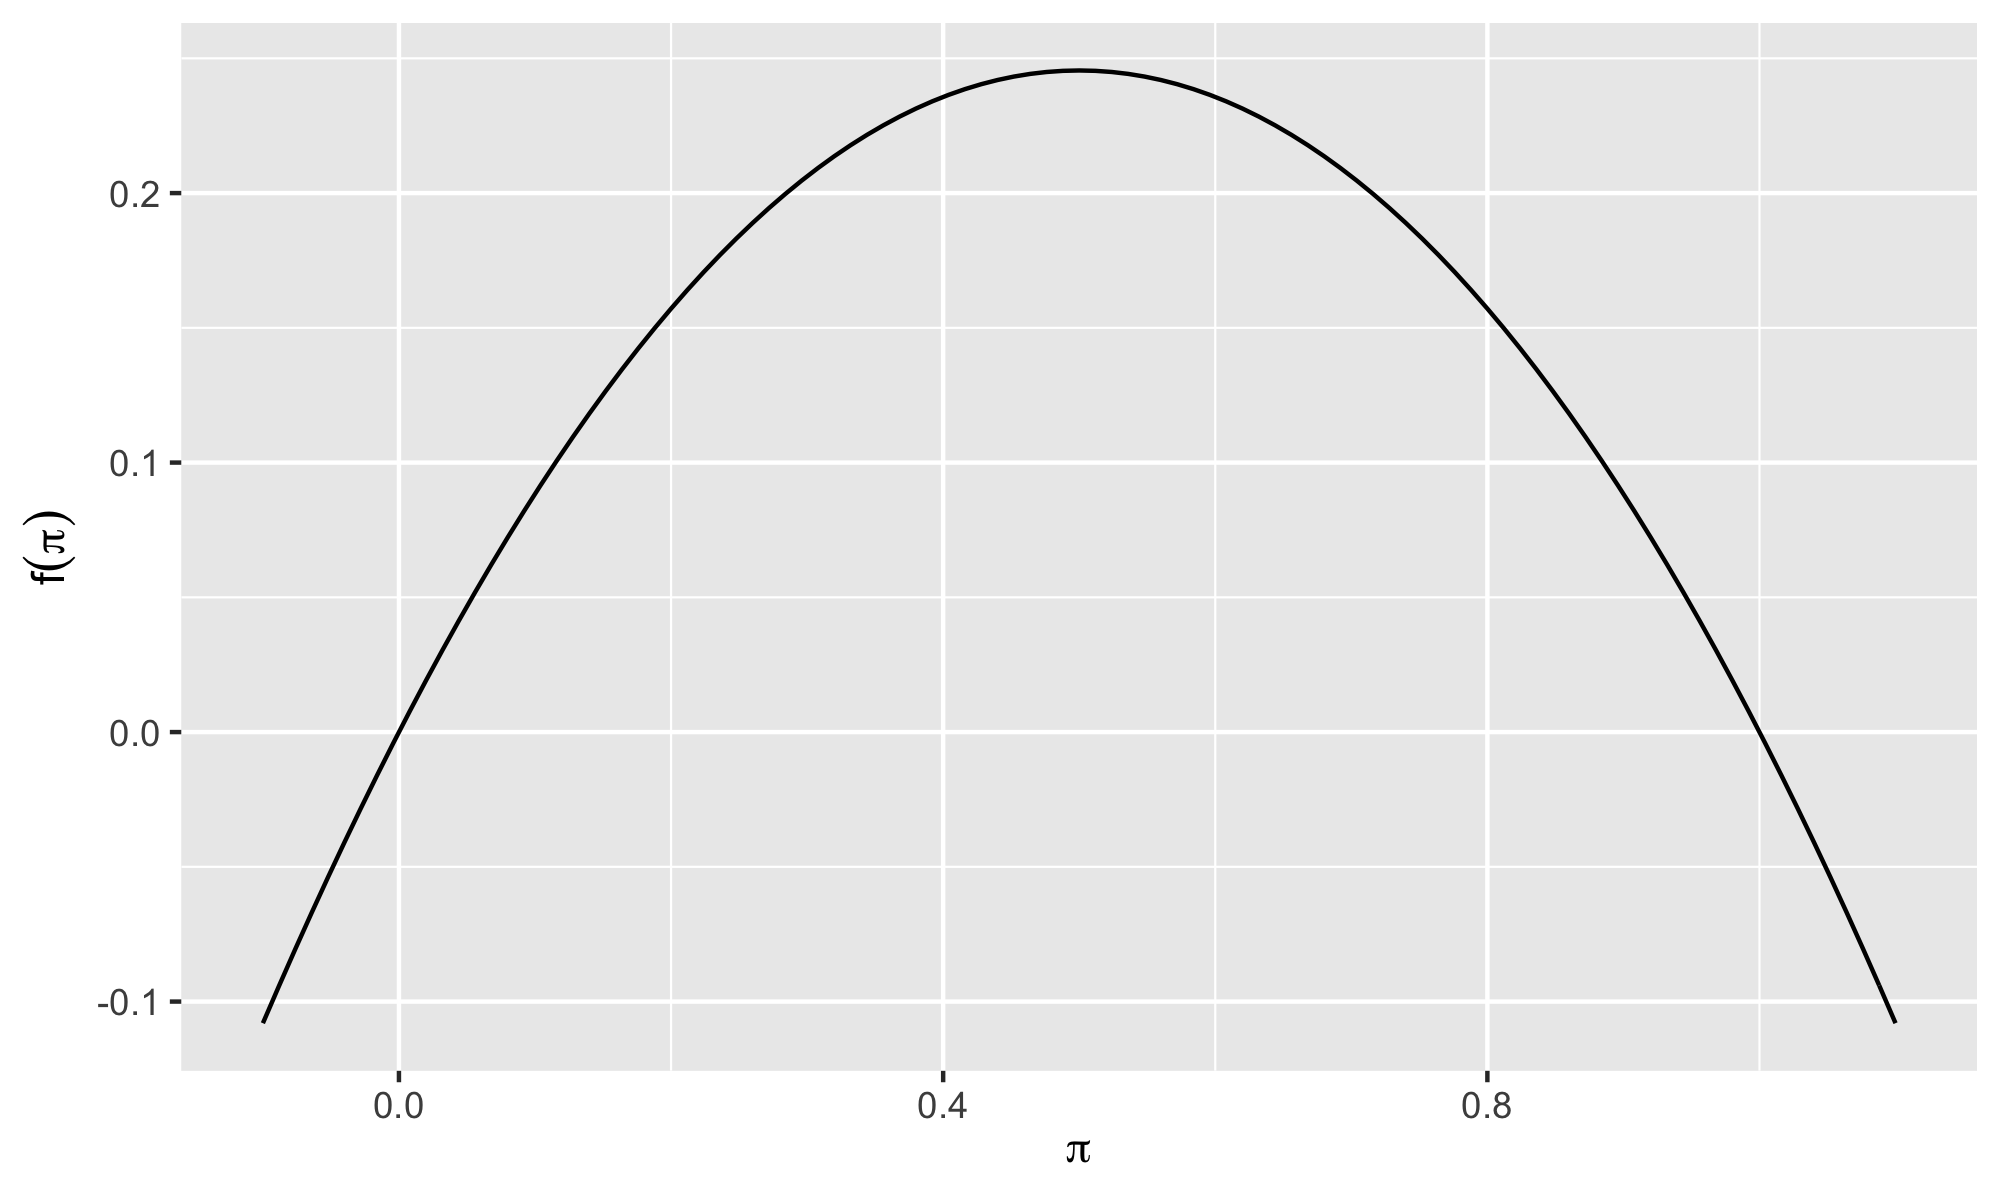
\includegraphics[width=12cm]{f-gate.png}

Similarly, \(LR(E)>1\) for any \(0< \pi <1\). Here is a plot of
\(LR(E)\) against \(\pi\):

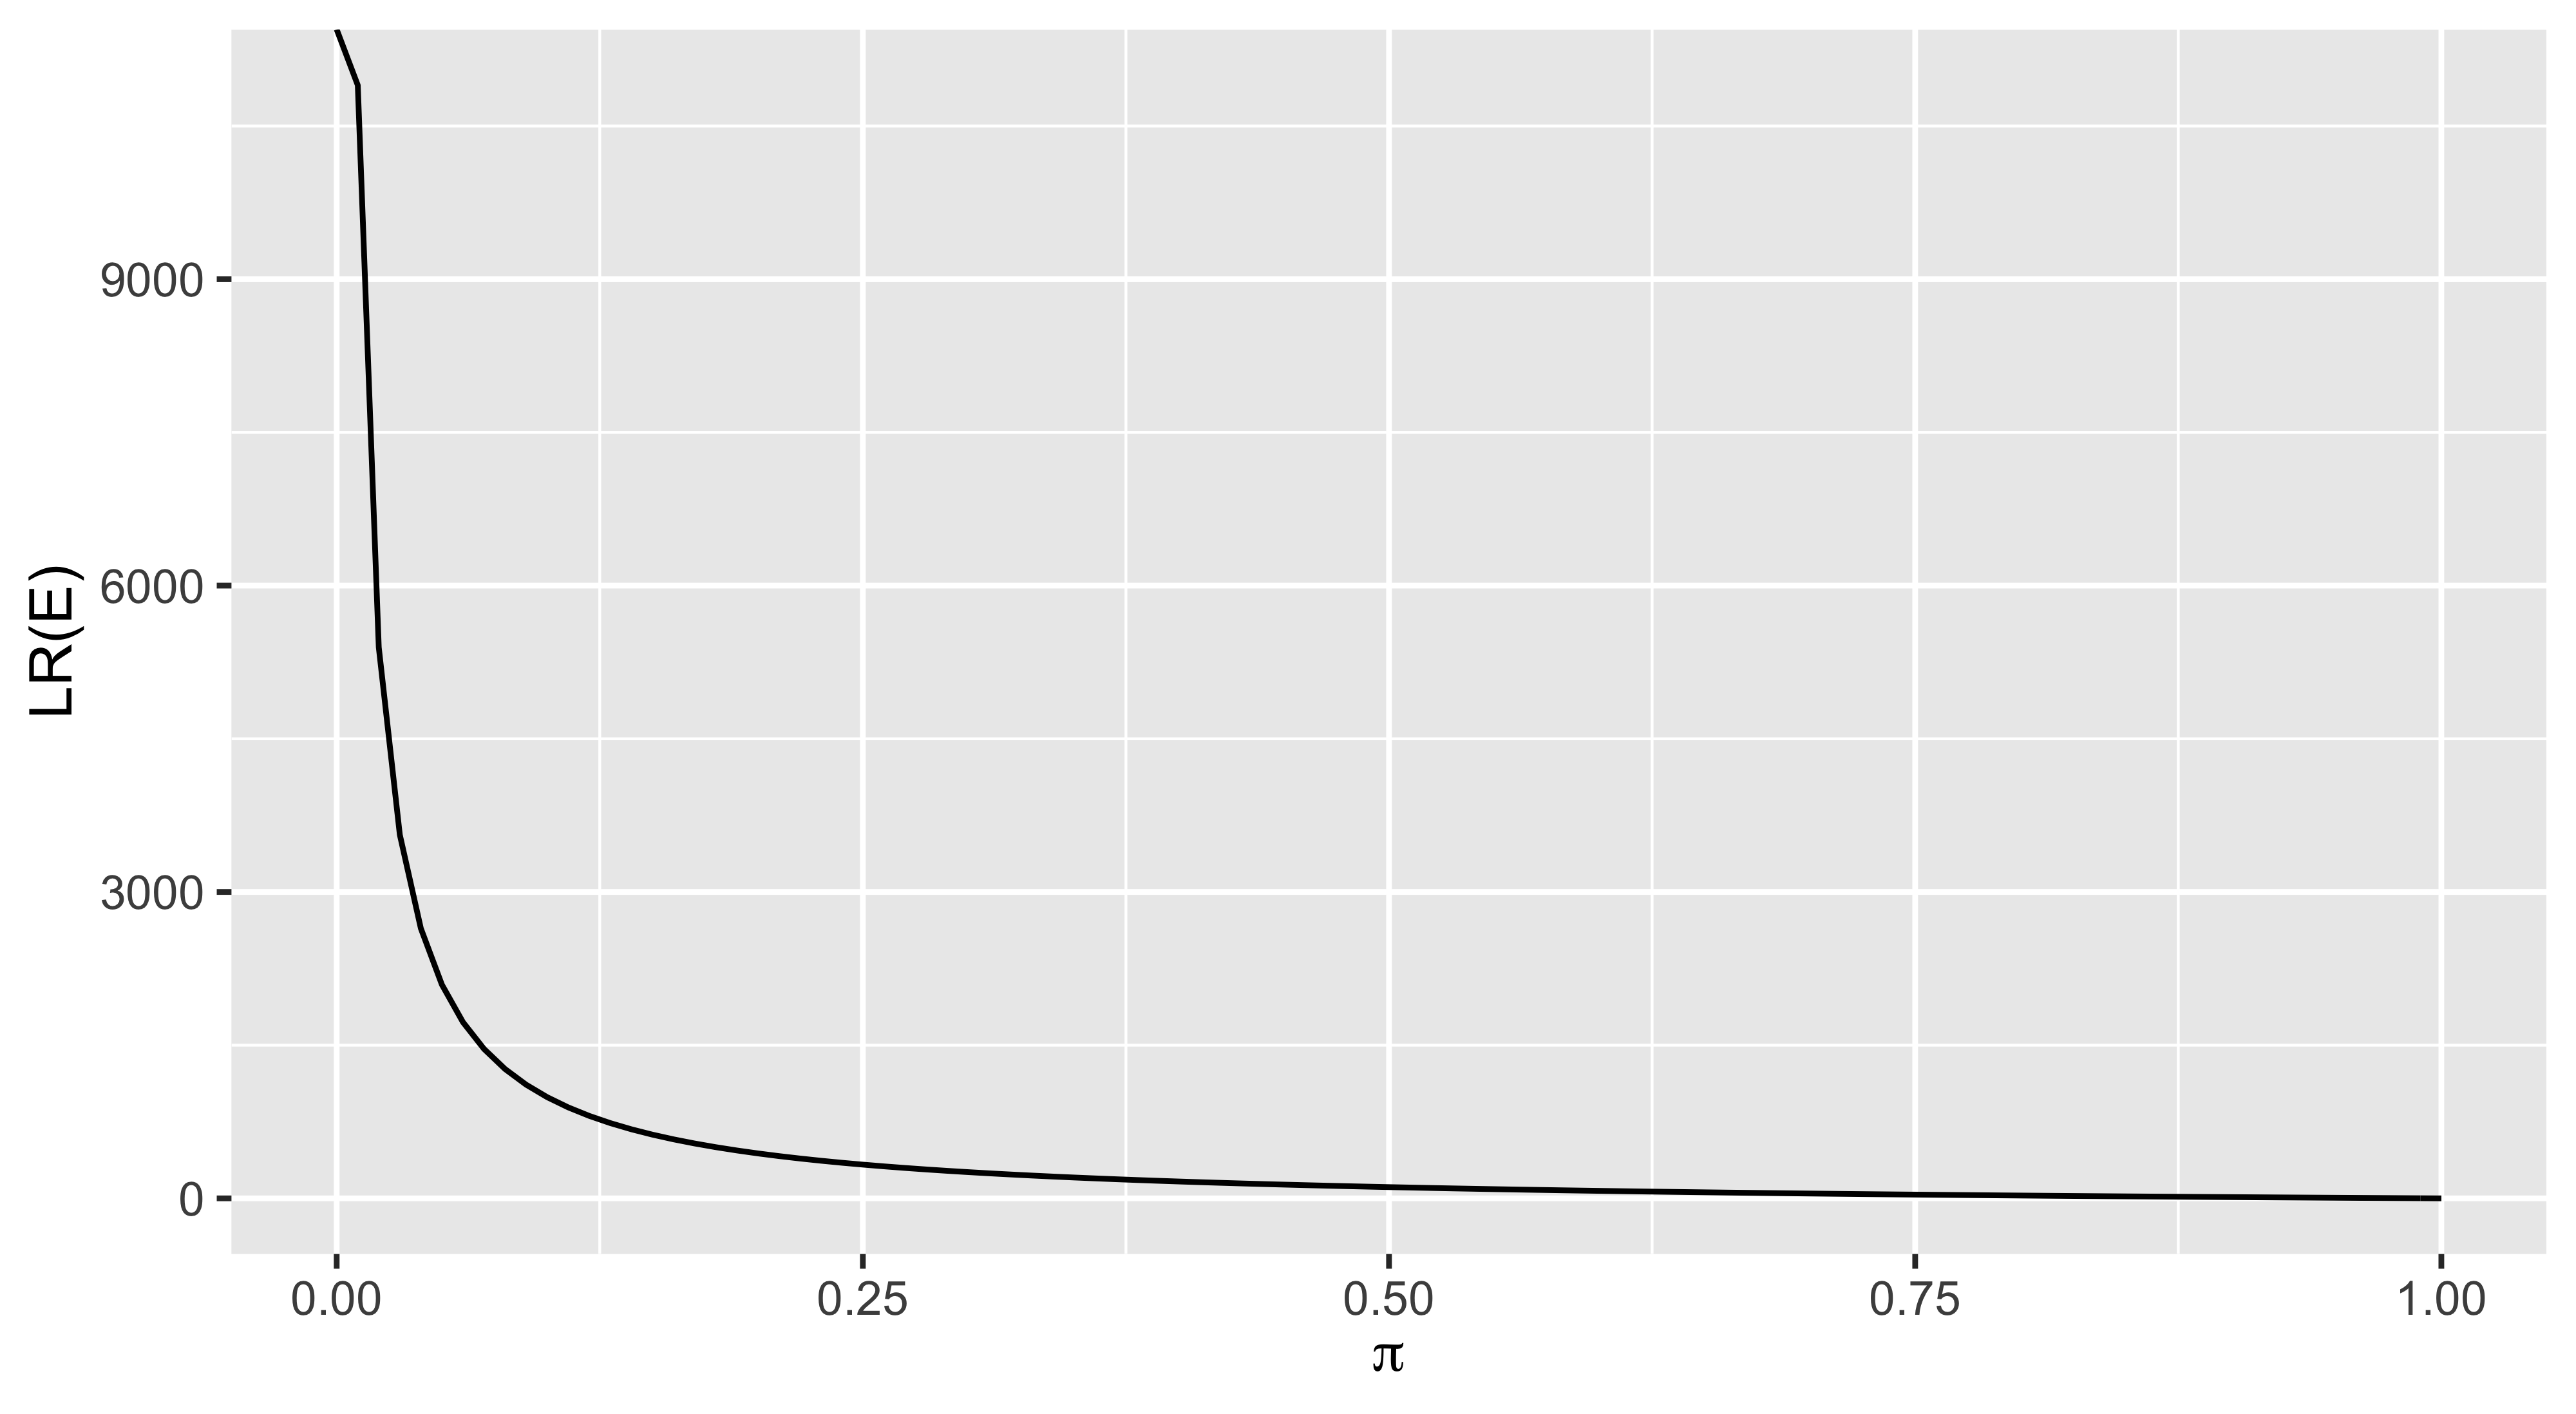
\includegraphics[width=12cm]{lre-gate.png}

\noindent Notice that \(LR(E)\) does not go below 1. This means that for
\(L=G\) in the gatecrasher scenario DTLP wold tell us to convict for any
prior probability of guilt \(\pi\neq 0,1\).

One might ask: is the conclusion very sensitive to the choice of \(L\)
and \(G\)? The answer is, not too much.

\intermezzoa

How sensitive is our analysis to the choice of \(L/G\)? Well, \(LR(E)\)
does not change at all, only the threshold moves. For instance, if
\(L/G=4\), instead of \(f\) we end up with \begin{align*}
 f'(\pi) = - 0.955 \pi^2 + 0.955\pi &>0 
 \end{align*} and the function still takes positive values on the
interval \((0,1)\). In fact, the decision won't change until \(L/G\)
increases to \(\approx 111\). Denote \(L/G\) as \(\rho\), and let us
start with the general decision standard, plugging in our calculations
for \(LR(E)\): \begin{align*}
LR(E) &> \frac{\pr{H_\Delta}}{\pr{H_\Pi}} \rho\\
LR(E) &> \frac{1-\pi}{\pi} \rho \\
\frac{0.991-0.991\pi}{0.009\pi} &> \frac{1-\pi}{\pi} \rho\\
\frac{0.991-0.991\pi}{0.009\pi}\frac{\pi}{1-\pi} &>  \rho\\
\frac{0.991\pi-0.991\pi^2}{0.009\pi-0.009\pi^2} &>  \rho\\
\frac{\pi(0.991-0.991\pi)}{\pi(0.009-0.009\pi)} &>  \rho\\
\frac{0.991-0.991\pi}{0.009-0.009\pi} &>  \rho\\
\frac{0.991(1-\pi)}{0.009(1-\pi)} &>  \rho\\
\frac{0.991}{0.009} &>  \rho\\
110.1111 &>  \rho\\
\end{align*}

\intermezzob

So, we conclude, in usual circumstances, DTLP does not handle the
gatecrasher paradox.

\hypertarget{conclusions}{%
\subsection{Conclusions}\label{conclusions}}

Where are we, how did we get here, and where can we go from here? We
were looking for a probabilistically explicated condition \(\Psi\) such
that the trier of fact, at least ideally, should accept any relevant
claim (including \(G\)) just in case \(\Psi(A,E)\).

From the discussion that transpired it should be clear that we were
looking for a \(\Psi\) satisfying the following desiderata:

\begin{description}
\item[conjunction closure] If $\Psi(A,E)$ and $\Psi(B,E)$, then $\Psi(A\et B,E)$.
\item[naked statistics] The account should at least make it possible for convictions based on strong, but naked statistical evidence to be unjustified. 
\item[equal treatment] the condition should apply to any relevant claim whatsoever (and not just a selected claim, such as $G$).
\end{description}

Throughout the paper we focused on the first two conditions (formulated
in terms of the difficulty about conjunction (DAC), and the gatecrasher
paradox), going over various proposals of what \(\Psi\) should be like
and evaluating how they fare. The results can be summed up in the
following table:

\begin{center}
\footnotesize 
 \begin{tabular}{@{}p{3cm}p{2.5cm}p{4cm}p{3cm}@{}}
\toprule
\textbf{View} & \textbf{Convict iff} & \textbf{DAC} & \textbf{Gatecrasher} \\ \midrule
Threshold-based LP (TLP) & Probability of guilt given the evidence is above a certain threshold & fails & fails \\
Dawid's likelihood strategy & No condition given, focus on $\frac{\pr{H\vert E}}{\pr{H\vert \n E}}$ & - If evidence is fairly reliable, the posterior of $A\et B$ will be greater than the prior.

- The posterior of $A\et B$ can still be lower than the posterior of any of $A$ and $B$.

- Joint likelihood, contrary do Dawid's claim, can also be lower than any of the individual likelihoods. & fails  \\
Cheng's relative LP (RLP)
& Posterior of guilt higher than the posterior of any of the defending narrations & The solution assumes equal costs of errors and independence of $A$ and $B$ conditional on $E$. It also relies on there being multiple defending scenarios individualized in terms of  combinations of literals involving $A$ and $B$. & Assumes that the prior odds of guilt are 1, and that the statistics is not sensitive to guilt (which is dubious). If the latter fails, tells to convict as long as the prior of guilt $<0.991$. \\
Kaplow's decision-theoretic LP (DTLP) &
The likelihood of the evidence is higher than the odds of innocence multiplied by the cost of error ratio & fails & convict if cost ratio $<110.1111$
\end{tabular} 
 \end{center}

Thus, each account either simply fails to satisfy the desiderata, or
succeeds on rather unrealistic assumptions. Does this mean that a
probabilistic approach to legal evidence evaluation should be abandoned?
No.~This only means that if we are to develop a general probabilistic
model of legal decision standards, we have to do better. One promising
direction is to go back to Cohen's pressure against
\textbf{Requirement 1} and push against it. A brief paper suggesting
this direction is (Di Bello, 2019), where the idea is that the
probabilistic standard (be it a threshold or a comparative wrt.
defending narrations) should be applied to the whole claim put forward
by the plaintiff, and not to its elements. In such a context, DAC does
not arise, but \textbf{equal treatment} is violated. Perhaps, there are
independent reasons to abandon it, but the issue deserves further
discussion. Another strategy might be to go in the direction of
employing probabilistic methods to explicate the narration theory of
legal decision standards (Urbaniak, 2018), but a discussion of how this
approach relates to DAC and the gatecrasher paradox lies beyond the
scope of this paper.

\hypertarget{references}{%
\section*{References}\label{references}}
\addcontentsline{toc}{section}{References}

\hypertarget{refs}{}
\begin{CSLReferences}{1}{0}
\leavevmode\hypertarget{ref-Allen1986A-Reconceptuali}{}%
Allen, R. J. (1986). A reconceptualization of civil trials. \emph{Boston
University Law Review}, \emph{66}, 401--437.

\leavevmode\hypertarget{ref-allen2013}{}%
Allen, R. J., \& Stein, A. (2013). Evidence, probability and the burden
of proof. \emph{Arizona Law Journal}, \emph{55}, 557--602.

\leavevmode\hypertarget{ref-AllenPardo2019relative}{}%
Allen, R., \& Pardo, M. (2019). Relative plausibility and its critics.
\emph{The International Journal of Evidence {\&} Proof}, \emph{23}(1-2),
5--59. \url{https://doi.org/10.1177/1365712718813781}

\leavevmode\hypertarget{ref-cheng2012reconceptualizing}{}%
Cheng, E. (2012). Reconceptualizing the burden of proof. \emph{Yale LJ},
\emph{122}, 1254.

\leavevmode\hypertarget{ref-Cohen1977The-probable-an}{}%
Cohen, J. L. (1977). \emph{The probable and the provable}. Oxford
University Press. \url{https://doi.org/10.2307/2219193}

\leavevmode\hypertarget{ref-cohen1988difficulty}{}%
Cohen, L. J. (1988). The difficulty about conjunction in forensic proof.
\emph{The Statistician}, \emph{37}(4/5), 415.
\url{https://doi.org/10.2307/2348767}

\leavevmode\hypertarget{ref-dawid1987difficulty}{}%
Dawid, A. P. (1987). The difficulty about conjunction. \emph{The
Statistician}, 91--97.

\leavevmode\hypertarget{ref-DiBello2019plausibility}{}%
Di Bello, M. (2019). Probability and plausibility in juridical proof.
\emph{International Journal of Evidence and Proof}.

\leavevmode\hypertarget{ref-haack2011legal}{}%
Haack, S. (2014). Legal probabilism: An epistemological dissent. In
\emph{{Haack2014-HAAEMS}} (pp. 47--77).

\leavevmode\hypertarget{ref-kaplow2014likelihood}{}%
Kaplow, L. (2014). Likelihood ratio tests and legal decision rules.
\emph{American Law and Economics Review}, \emph{16}(1), 1--39.

\leavevmode\hypertarget{ref-Kowalewska2021conjunction}{}%
Kowalewska, A. (2021). Reasoning without the conjunction closure.
\emph{Episteme}, 1--14. \url{https://doi.org/10.1017/epi.2020.53}

\leavevmode\hypertarget{ref-Makinson1965-MAKTPO-2}{}%
Makinson, D. C. (1965). The paradox of the preface. \emph{Analysis},
\emph{25}(6), 205--207.

\leavevmode\hypertarget{ref-schwartz2017ConjunctionProblemLogic}{}%
Schwartz, D. S., \& Sober, E. R. (2017). The {Conjunction Problem} and
the {Logic} of {Jury Findings}. \emph{William \& Mary Law Review},
\emph{59}(2), 619--692.

\leavevmode\hypertarget{ref-Stein05}{}%
Stein, A. (2005). \emph{Foundations of evidence law}. Oxford University
Press.

\leavevmode\hypertarget{ref-urbaniak2018narration}{}%
Urbaniak, R. (2018). Narration in judiciary fact-finding: A
probabilistic explication. \emph{Artificial Intelligence and Law},
1--32. \url{https://doi.org/10.1007/s10506-018-9219-z}

\end{CSLReferences}

\end{document}
